\documentclass[a4paper]{article}

\usepackage[latin1]{inputenc}
\usepackage{bbm}
\usepackage{amsmath,amsthm,amssymb}
\usepackage{graphicx,color}

% to change the margins.  Default for 12pt is 1.5in
%\usepackage[margin=1.1in]{geometry}

\usepackage{amsmath,amssymb,amsthm}
\usepackage{MnSymbol}
\usepackage{graphicx,subfigure}
\usepackage[usenames,dvipsnames]{xcolor} % for more colors


% references

\newcommand{\secref}[1]{Section~\ref{sec:#1}}
\newcommand{\figref}[1]{Figure~\ref{fig:#1}}


% operator

\DeclareMathOperator{\co}{co}
\DeclareMathOperator{\diag}{diag}
\DeclareMathOperator{\dist}{dist}
\DeclareMathOperator*{\argmin}{argmin}
\DeclareMathOperator*{\argmax}{argmax}
\DeclareMathOperator{\vol}{vol}
\DeclareMathOperator{\linspan}{span}
\DeclareMathOperator{\id}{id}


% editing
\usepackage{color}
\newcommand{\comment}[1] {\textbf{\color{red} [#1]}}
\newcommand{\change} [1] {{\color{blue} #1}}
\newcommand{\changeme}[1]{{\sc \color{Orange} [#1]}}


%commands

\newcommand{\dby}[1]{\partial_{#1}}
\newcommand{\vint}[1]{\langle #1 \rangle}
\newcommand{\vvint}[1]{\llangle #1 \rrangle}
\newcommand{\Vint}[1]{\left\langle #1 \right\rangle}
\newcommand{\VVint}[1]{\left\llangle #1 \right\rrangle}
\newcommand{\sig}[1]{\sigma_{\mathrm{#1}}}
\newcommand{\itembf}[1]{\item \textbf{#1}}


% for mean-value integrals (use \dashint or \ddashint):
\def\Xint#1{\mathchoice
{\XXint\displaystyle\textstyle{#1}}%
{\XXint\textstyle\scriptstyle{#1}}%
{\XXint\scriptstyle\scriptscriptstyle{#1}}%
{\XXint\scriptscriptstyle\scriptscriptstyle{#1}}%
\!\int}
\def\XXint#1#2#3{{\setbox0=\hbox{$#1{#2#3}{\int}$ }
\vcenter{\hbox{$#2#3$ }}\kern-.6\wd0}}
\def\ddashint{\Xint=}
\def\dashint{\Xint-}


% shorthands

\def\Diag{\operatorname{Diag}}
\def\minimize{\operatorname*{minimize}}
\def\st{\operatorname*{subject~to}}
\def\quand{\quad \mbox{and} \quad}
\def\p{\partial}
\def\grad{\nabla}
\def\veps{\varepsilon}
\def\vphi{\varphi}
\def\root3{\sqrt{3}}
\def\SN{\text{S}_N}
\def\PN{\text{P}_N}
\def\MN{\text{M}_N}
\def\dt{\Delta t}
\def\dx{\Delta x}
\def\dy{\Delta y}
\def\dz{\Delta z}
\def\siga{\sig{a}}
\def\sigs{\sig{s}}
\def\sigt{\sig{t}}

\def\divg{\grad \cdot}
\def\divx{\grad_x \cdot}
\def\curl{\grad \times}

\def\nin{\not \in}

\def\intd{\, d}
\def\intdv{\intd v}
\def\intdw{\intd w}
\def\intdx{\intd x}
\def\intdS{\intd S(\Omega)}

\def\St{\text{St}}
\def\Kn{\text{Kn}}

\def\ba{\mathbf{a}}
\def\bb{\mathbf{b}}
\def\bc{\mathbf{c}}
\def\bd{\mathbf{d}}
\def\be{\mathbf{e}}
\def\bff{\mathbf{f}}
\def\bg{\mathbf{g}}
\def\bh{\mathbf{h}}
\def\bi{\mathbf{i}}
\def\bj{\mathbf{j}}
\def\bk{\mathbf{k}}
\def\bl{\mathbf{l}}
\def\bm{\mathbf{m}}
\def\bn{\mathbf{n}}
\def\bo{\mathbf{o}}
\def\bp{\mathbf{p}}
\def\bq{\mathbf{q}}
\def\br{\mathbf{r}}
\def\bs{\mathbf{s}}
\def\bt{\mathbf{t}}
\def\bu{\mathbf{u}}
\def\bv{\mathbf{v}}
\def\bw{\mathbf{w}}
\def\bx{\mathbf{x}}
\def\by{\mathbf{y}}
\def\bz{\mathbf{z}}

\def\bA{\mathbf{A}}
\def\bB{\mathbf{B}}
\def\bC{\mathbf{C}}
\def\bD{\mathbf{D}}
\def\bE{\mathbf{E}}
\def\bF{\mathbf{F}}
\def\bG{\mathbf{G}}
\def\bH{\mathbf{H}}
\def\bI{\mathbf{I}}
\def\bJ{\mathbf{J}}
\def\bK{\mathbf{K}}
\def\bL{\mathbf{L}}
\def\bM{\mathbf{M}}
\def\bN{\mathbf{N}}
\def\bO{\mathbf{O}}
\def\bP{\mathbf{P}}
\def\bQ{\mathbf{Q}}
\def\bR{\mathbf{R}}
\def\bS{\mathbf{S}}
\def\bT{\mathbf{T}}
\def\bU{\mathbf{U}}
\def\bV{\mathbf{V}}
\def\bW{\mathbf{W}}
\def\bX{\mathbf{X}}
\def\bY{\mathbf{Y}}
\def\bZ{\mathbf{Z}}

\def\cA{\mathcal{A}}
\def\cB{\mathcal{B}}
\def\cC{\mathcal{C}}
\def\cD{\mathcal{D}}
\def\cE{\mathcal{E}}
\def\cF{\mathcal{F}}
\def\cG{\mathcal{G}}
\def\cH{\mathcal{H}}
\def\cI{\mathcal{I}}
\def\cJ{\mathcal{J}}
\def\cK{\mathcal{K}}
\def\cL{\mathcal{L}}
\def\cM{\mathcal{M}}
\def\cN{\mathcal{N}}
\def\cO{\mathcal{O}}
\def\cP{\mathcal{P}}
\def\cQ{\mathcal{Q}}
\def\cR{\mathcal{R}}
\def\cS{\mathcal{S}}
\def\cT{\mathcal{T}}
\def\cU{\mathcal{U}}
\def\cV{\mathcal{V}}
\def\cW{\mathcal{W}}
\def\cX{\mathcal{X}}
\def\cY{\mathcal{Y}}
\def\cZ{\mathcal{Z}}

\def\bbA{\mathbb{A}}
\def\bbB{\mathbb{B}}
\def\bbC{\mathbb{C}}
\def\bbD{\mathbb{D}}
\def\bbE{\mathbb{E}}
\def\bbF{\mathbb{F}}
\def\bbG{\mathbb{G}}
\def\bbH{\mathbb{H}}
\def\bbI{\mathbb{I}}
\def\bbJ{\mathbb{J}}
\def\bbK{\mathbb{K}}
\def\bbL{\mathbb{L}}
\def\bbM{\mathbb{M}}
\def\bbN{\mathbb{N}}
\def\bbO{\mathbb{O}}
\def\bbP{\mathbb{P}}
\def\bbQ{\mathbb{Q}}
\def\bbR{\mathbb{R}}
\def\bbS{\mathbb{S}}
\def\bbT{\mathbb{T}}
\def\bbU{\mathbb{U}}
\def\bbV{\mathbb{V}}
\def\bbW{\mathbb{W}}
\def\bbX{\mathbb{X}}
\def\bbY{\mathbb{Y}}
\def\bbZ{\mathbb{Z}}

\def\bsalpha{\boldsymbol{\alpha}}
\def\bsbeta{\boldsymbol{\beta}}
\def\bsgamma{\boldsymbol{\gamma}}
\def\bsdelta{\boldsymbol{\delta}}
\def\bsvarepsilon{\boldsymbol{\varepsilon}}
\def\bszeta{\boldsymbol{\zeta}}
\def\bseta{\boldsymbol{\eta}}
\def\bstheta{\boldsymbol{\theta}}
\def\bsvarteta{\boldsymbol{\vartheta}}
\def\bsiota{\boldsymbol{\iota}}
\def\bskappa{\boldsymbol{\kappa}}
\def\bslambda{\boldsymbol{\lambda}}
\def\bsmu{\boldsymbol{\mu}}
\def\bsnu{\boldsymbol{\nu}}
\def\bsxi{\boldsymbol{\xi}}
\def\bspi{\boldsymbol{\pi}}
\def\bsvarpi{\boldsymbol{\varpi}}
\def\bsrho{\boldsymbol{\rho}}
\def\bsvarrho{\boldsymbol{\varrho}}
\def\bssigma{\boldsymbol{\sigma}}
\def\bsvarsigma{\boldsymbol{\varsigma}}
\def\bstau{\boldsymbol{\tau}}
\def\bsupsilon{\boldsymbol{\upislon}}
\def\bsphi{\boldsymbol{\phi}}
\def\bsvarphi{\boldsymbol{\varphi}}
\def\bschi{\boldsymbol{\chi}}
\def\bspsi{\boldsymbol{\psi}}
\def\bsomega{\boldsymbol{\omega}}

\def\bsGamma{\boldsymbol{\Gamma}}
\def\bsDelta{\boldsymbol{\Delta}}
\def\bsTheta{\boldsymbol{\Theta}}
\def\bsLambda{\boldsymbol{\Lambda}}
\def\bsXi{\boldsymbol{\Xi}}
\def\bsPi{\boldsymbol{\Pi}}
\def\bsSigma{\boldsymbol{\Sigma}}
\def\bsUpsilon{\boldsymbol{\Upsilon}}
\def\bsPhi{\boldsymbol{\Phi}}
\def\bsPsi{\boldsymbol{\Psi}}
\def\bsOmega{\boldsymbol{\Omega}}


\theoremstyle{plain}% default
\newtheorem{prop}{Proposition}
\newtheorem{cor}{Corollary}
\newtheorem{definition}{Definition}
\newtheorem{lemma}{Lemma}
\newtheorem{thm}{Theorem}

\theoremstyle{remark}
\newtheorem*{remark}{Remark}
\newtheorem*{remarks}{Remarks}

\bibliographystyle{plain}

\parindent 10pt
\setlength{\textwidth}{420pt}
\setlength{\oddsidemargin}{28pt}
\setlength{\topmargin}{0pt}
\setlength{\textheight}{620pt}

% The code that makes the article title is so horrible that it must
% be hidden in its own file.  The horribleness is because of the 
% need to handle multiple authors. 

\NeedsTeXFormat{LaTeX2e}
\ProvidesPackage{nmd/title}[2014/08/31 - Semester start edition]

% Code for names, title, etc.  Mostly taken from amsart
% Save the title
\renewcommand{\title}[2][]{\gdef\@title{#2}}
% Formating for addresses at the end
\newcommand{\nmd@author}[1]{#1\par}
\newcommand{\nmd@address}[1]{#1\par}
\newcommand{\nmd@email}[1]{email: \texttt{#1}\par}
\newcommand{\nmd@urladdr}[1]{\url{#1}\par \vspace{10bp}}
% For combining the authors names, we need this giant mess
\let\@xp=\expandafter
\let\@nx=\noexpand
\long\def\@ifempty#1{\@xifempty#1@@..\@nil}
\long\def\@xifempty#1#2@#3#4#5\@nil{%
  \ifx#3#4\@xp\@firstoftwo\else\@xp\@secondoftwo\fi}
\long\def\@ifnotempty#1{\@ifempty{#1}{}}
\csname newtoks\endcsname\@emptytoks
\newcommand{\xandlist}[4]{\@andlista{{#1}{#2}{#3}}#4\and\and}
\def\@andlista#1#2\and#3\and{\@andlistc{#2}\@ifnotempty{#3}{%
    \@andlistb#1{#3}}}
\def\@andlistb#1#2#3#4#5\and{%
  \@ifempty{#5}{%
    \@andlistc{#2#4}%
  }{%
    \@andlistc{#1#4}\@andlistb{#1}{#3}{#3}{#5}%
  }}
\let\@andlistc\@iden
\newcommand{\nxandlist}[4]{%
  \def\@andlistc##1{\toks@\@xp{\the\toks@##1}}%
  \toks@{\toks@\@emptytoks \@andlista{{#1}{#2}{#3}}}%
  \the\@xp\toks@#4\and\and
  \edef#4{\the\toks@}%
  \let\@andlistc\@iden}
\def\@@and{and}
\newcommand{\andify}{%
  \nxandlist{\unskip, }{\unskip{} \@@and~}{\unskip, \@@and~}}
\def\and{\unskip{ }\@@and{ }\ignorespaces}
% End giant mess

\let\authors\@empty
\let\addresses\@empty
\renewcommand{\author}[2][]{%
  \ifx\@empty\authors
  \gdef\authors{#2}%
  \gdef\addresses{\nmd@author{#2}}
  \else
  \g@addto@macro\authors{\and#2}%
  \g@addto@macro\addresses{\nmd@author{#2}}%
  \fi
}%
% Save addresses, emails, and urls.
\newcommand{\address}[2][]{%
  \g@addto@macro\addresses{\nmd@address{#2}}}
\newcommand{\email}[2][]{%
  \g@addto@macro\addresses{\nmd@email{#2}}}
\newcommand{\urladdr}[2][]{%
  \g@addto@macro\addresses{\nmd@urladdr{#2}}}
% The abstract.  
\newsavebox\abstractbox
\renewenvironment{abstract}{%
  \global\setbox\abstractbox=\vtop \bgroup%
  \begin{leftruledparagraph}{3bp}{8bp}{nmdmedium}
    \textbf{Abstract.} }
  {\end{leftruledparagraph}\egroup}

% The dedication 
\newsavebox\dedicationbox
\newenvironment{dedication}{%
  \global\setbox\dedicationbox=\vtop \bgroup%
  \begin{center} \dedicationfont
   }
{\end{center}\egroup}


\def\maketitle{\par
  \@topnum\z@ % this prevents figures from falling at the top of page 
  \thispagestyle{empty}
  
  \
  
  \vspace{20bp}
  
  {\titlefont\setlength{\baselineskip}{30bp}
    \noindent
    \@title
    
  }
  
  \vspace{40bp}
  \noindent
  \andify\authors 
  {\authorfont \authors}
  \vspace{10bp}
  
  \noindent
  \usebox{\dedicationbox}

  \noindent
  \usebox{\abstractbox}
}
\AtEndDocument{%
  \small 
  \interlinepenalty\@M
  \setlength{\parindent}{0pt}
  \ifaddress \addresses \fi
}


\begin{document}
\maketitle

%!TEX root = AppM2_MultiD.tex

\begin{abstract}
  We extend to three-dimensional space the approximate $M_2$ model for
  the slab geometry studied in \cite{alldredge2016approximating}. The
  $B_2$ model therein, as a special case of the second order extended
  quadrature method of moments (EQMOM), is proved to be globally
  hyperbolic. The model we propose here extends EQMOM to multiple
  dimensions following the idea to approximate the maximum entropy
  closure for the slab geometry case. Like the $M_2$ closure, the
  ansatz of the new model has the capacity to capture both isotropic
  and beam-like solutions. Also, the new model has fluxes in
  closed-form; thus, it is applicable to practical numerical
  simulations. The rotational invariance, realizability, and
  hyperbolicity of the model are studied.
\end{abstract}

Keywords: Radiative transfer, moment model, maximum entropy closure

%%% Local Variables: 
%%% mode: latex
%%% TeX-master: "AppM2_MultiD.tex"
%%% End: 



\newcommand{\R}{\mathbb{R}}
\newcommand{\hdist}{\mathsf{hdist}}
\newcommand{\mdist}{\mathsf{mdist}}
\section{Introduction}

A homogeneous polynomial $p$ in $\R[x_1,\ldots,x_n]$ is said to be {\em hyperbolic} with respect to a direction $e \in \R^n$ if $p(e)\neq 0$ and all its univariate restrictions along the direction $e$ are real-rooted, i.e., for every $x \in \R^n$, the polynomial $p_x(t) = p(t e + x)$ has all real roots.
%
G\aa rding showed that every hyperbolic polynomial $p$ is associated with a closed\footnote{The usual definition considers open cones, but we will work with their closures instead.} convex cone $K_p$ defined as follows,
\[ K_p = \{x \in \R^n | \text{ all roots of } p(te + x) \text{ are non-positive} \}. \]
%
The cone $K_p$ is referred to as the hyperbolicity cone associated with the polynomial $p$.  

From the standpoint of convex optimization, hyperbolicity cones yield a rich
family of convex sets that one can efficiently optimize over --- in particular,
interior point methods can be used to efficiently optimize over the
hyperbolicity cone $K_p$ for a polynomial $p$, given an oracle to evaluate $p$
and its gradient and Hessian \cite{guler1997,renegar2006hyperbolic}. This
optimization primitive,  referred to as {\it hyperbolic programming}, captures
linear and semidefinite programming as special cases.  Specifically, the
hyperbolicity cone for the polynomial $p(x_1,\ldots,x_n) = \prod_{i = 1}^n x_i$
is the positive orthant $\R_+^n$, which corresponds to linear programming, while
semidefinite programming arises from the symmetric determinant polynomial
$\det(X)$. 
Is hyperbolic programming as an algorithmic primitive strictly more
 powerful than semidefinite programming?
Can hyperbolicity cones other than these two be harnessed towards obtaining
 better algorithms for combinatorial optimization problems?  These compelling questions remain
 open.  

Lately, the relationship between hyperbolicity cones and the semidefinite cone has been a subject
of intense study. It is easy to see that every section of the semidefinite cone is a hyperbolicity cone, so it is natural to ask
whether the converse holds, i.e., if every
hyperbolicity cone can be realized as a section of the semidefinite cone.
Formally, a {\it spectrahedral cone} $K$ is specified by:
$$ K = \{ x \in \R^n \mid \sum_i A_i x_i \succeq 0 \},$$ for some matrices $\{A_i\}_{i \in [n]} \in
\R^{B \times B}$.  It is conjectured that every hyperbolicity cone is a
spectahedral cone.

\begin{conjecture} (Generalized Lax Conjecture)
Every hyperbolicity cone is a spectahedral cone, i.e., a linear section of the cone of positive semidefinite matrices in some dimension.
\end{conjecture}

The Lax conjecture in its original stronger algebraic form asked whether every
polynomial in three variables hyperbolic with respect to the
direction $(1,0,0)$, could be written as $\det(xI+yB+zC)$ for some symmetric
matrices $B,C$ (sometimes called a {\em definite determinantal representation}). This immediately implies that all hyperbolicity cones in three
dimensions are spectrahedral, and was proved by Helton and Vinnikov and Lewis,
Parrilo, and Ramana \cite{helton2007linear,lewis2005lax}. The algebraic
conjecture is easily seen to be false for $n>3$ by a count of parameters, since
the set of hyperbolic polynomials is known to have nonempty interior
\cite{nuij1969note} and is of dimension $n^d$, whereas the set of $n-$tuples of
$d\times d$ matrices has dimension $n\binom{d}{2}$. This led to the weaker
conjecture that for every hyperbolic $p(x)$ there is an integer $k$ such that
$p(x)^k$ admits a definite determinantal representation, which was disproved by Br\"anden in \cite{branden2011obstructions}.
The Generalized Lax conjecture, which is a geometric statement, is equivalent to the yet weaker algebraic statement
that for every hyperbolic $p(x)$ there is a hyperbolic $q(x)$ such that $K_p\subseteq K_q$ and
$p(x)q(x)$ admits a definite determinantal representation.

For several special classes of hyperbolic polynomials, the corresponding
hyperbolicity cones are known to be spectrahedral.  The elementary
symmetric polynomial of degree $d$ in $n$ variables is given by $e_d(x) =
\sum_{S \subseteq [n], |S| = d} \prod_{i \in S} x_i$. Br\"anden \cite{branden2014hyperbolicity} 
 showed that the hyperbolicity cones of
elementary symmetric polynomials are spectrahedral with matrices of dimension $O(n^d)$.  If a polynomial $p$ is
hyperbolic with respect to a direction $e \in \R^n$, then its directional
derivatives along $e$ are hyperbolic too \cite{gaarding1959inequality}.
Directional derivatives of the polynomial $p(x) = \prod_{i \in [n]} x_i$
\cite{zinchenko2008hyperbolicity,sanyal2013derivative,branden2014hyperbolicity,choe2004homogeneous}
and the first derivatives of the determinant polynomial \cite{saunderson2017spectrahedral} are also known to
satisfy the generalized Lax conjecture. Amini \cite{amini2016spectrahedrality} has shown that 
certain multivariate matching polynomials are hyperbolic and that their cones are spectrahedral, of
dimension $n!$. 

Given the above examples, it is natural to wonder whether exponential
blowup in dimension is an essential feature of passing from hyperbolicity cones
to spectrahedral representations, and even assuming the generalized Lax conjecture to be
true, the size of the spectrahedral representation of a hyperbolicity cone is
interesting from a complexity standpoint. 
In this paper, we obtain exponential lower bounds on the size of the spectrahedral representation in general, even if
the representation is allowed to be approximate (up to an exponentially small error).

Recall that the Hausdroff distance between two cones
		$K$ and $K'$ is defined as $$\hdist(K,K') = \max_{x \in
		\mathcal{B} \cap K, y \in \mathcal{B} \cap K'} (d(x,K'),
		d(y,K)),$$ where $\mathcal{B}$ is the unit ball in $\R^n$.
We say that a spectrahedral cone $K'$ is  an {\em $\eta$-approximate spectrahedral representation} of another cone $K$ if
$\hdist(K,K')\le \eta$.
Our main theorem is the following.
\begin{theorem} [Main Theorem]\label{thm:main}
There exists an absolute constant $\kappa > 0$ such that for all sufficiently large $n, d$, 
there exists an n-variate degree $d$ hyperbolic polynomial $p$ whose hyperbolicity cone $K_p$ does not admit an $\eta-$approximate spectrahedral representation of dimension $B \leq \left(n/ d\right)^{\kappa d}$, for $\eta=1/n^{4nd}$. 
\end{theorem}

Our proof is analytic and does not rely on algebraic obstacles to
representability; in fact the polynomials we construct have very simple
coefficients (they are essentially binary perturbations of $e_d$).  However,
since there are $\binom{n}{d}$ coefficients, the examples require $\Omega(n^d)$
bits to write down. It is still unknown whether $e_d$ itself admits a low dimensional spectrahedral
representation, though Saunderson and Parrilo \cite{saunderson2015polynomial} have shown that if one allows
{\em projections} of sections of semidefinite cones, then such a represntation 
exists with size $\mathrm{poly}(n,d)$. 

Algebraically, the notion of (exact) spectrahedral representation of a
hyperbolicity cone $K_p$ for a polynomial $p$ corresponds to an algebraic
identity of the form, \[ p (x) \cdot q(x) = det ( \sum_{i \in [n]} C_i x_i) \ ,
\] where $K_q$ contains $K_p$.  Thus, our main theorem implies the existence of
a degree $d$ polynomial $p$ such that the degree of any identity of the above
form is at least $(n/d)^{\kappa d}$.


\subsection{Proof Overview}

The starting point for our proof is the theorem of Nuij \cite{nuij1969note},
which says that the space of hyperbolic polynomials of degree $d$ in $n$
variables has a nonempty interior, immediately implying that it has dimension
$n^d$. The Generalized Lax Conjecture concerns the {\em cones} of these
polynomials, which are geometric rather than algebraic objects. If we could
show that this space of cones also has large ``dimension'' in some appropriate quantitative
sense, and that the maps between the hyperbolicity cones and their spectrahedral representations are 
suitably well-behaved, then it would rule out the existence of small spectrahedral
representations for all of them uniformly, since such representations are parameterized
by tuples of $n$  $B\times B$ matrices, which have dimension $nB^2$. 

The difficulties in turning this idea into a proof are: (1) There are no
quantitative bounds on Nuij's theorem. (2) the space of hyperbolicity cones is
hard to parameterize and it is not clear how to define dimension. (3) the
mapping from hyperbolicity cones to their representations can be arbitrary, and
needn't preserve the usual notions of dimension anyway. We surmount these
difficulties by a packing argument, which consists of the following steps.

\begin{figure}
	\centering
	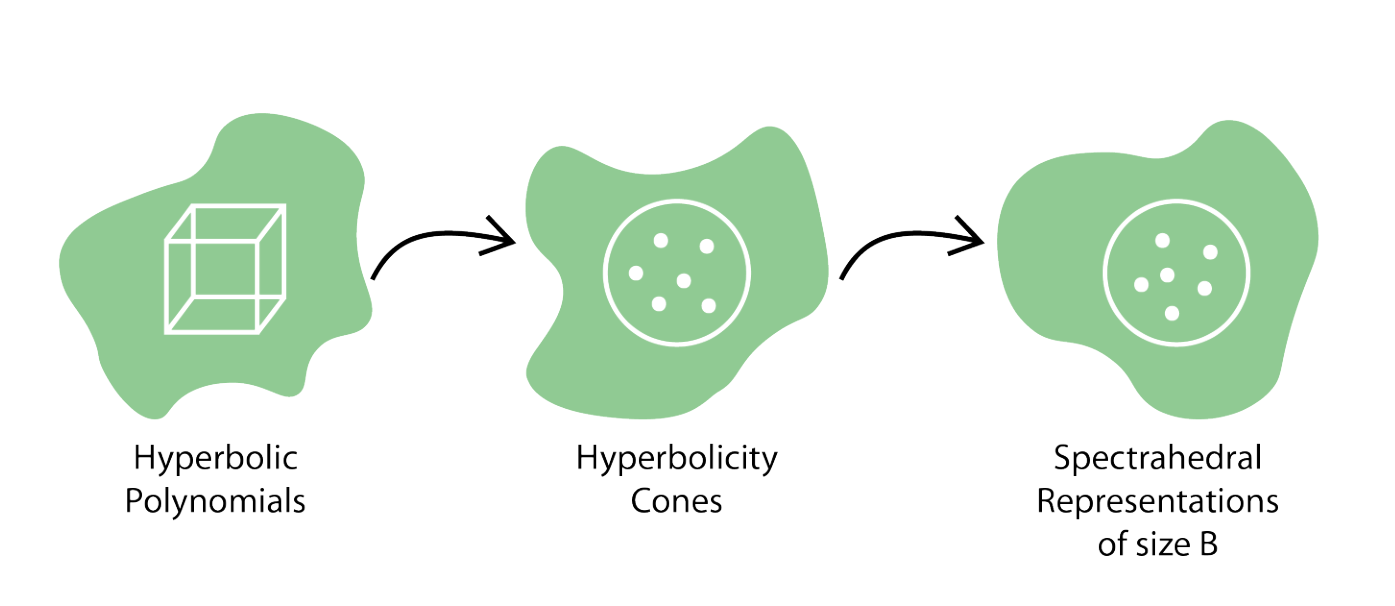
\includegraphics[width=0.8\textwidth]{diagram.PNG}
	\caption{Outline of the Proof}
\end{figure}

\begin{enumerate}
	\item Exhibit a large family of hyperbolicity cones of size
		$2^{(n/d)^{\Omega(d)}}$, every pair of which are at least
		$\epsilon$ apart from each other in the Hausdroff metric
		between the cones.  

\item  Show that the spectrahedral representations of two distant cones $K$ and
	$K'$ are distant from each other, once the representations are
		appropriately normalized.  Formally, the matrices $\{C_i\}_{i
		\in [n]}$ and $\{C'_i\}_{i \in [n]}$ representing the two cones
		are at least $\epsilon'$ away in operator norm if $\hdist(K,K')
		\geq \epsilon$ (see Lemma \ref{lem:conetomatrices}). 

		We work only with cones which contain the positive orthant in order to ensure
		that they have normalized representations.

\item By considering the volume, there is a $(B/\epsilon')^{nB^2}$ upper bound
	on the number of pairwise $\epsilon'$-distant spectrahedral
		representations in $B\times B$ matrices, thus giving the lower
		bound on $B$.

\end{enumerate}

By far, the most technical part of the proof is the first step exhibiting a large family of pairwise distant hyperbolicity cones.  
%
The set of hyperbolic polynomials is known to have a non-empty interior in the
set of all degree $d$ homogenous polynomials.  Although this implies the
existence of a full-dimensional family of hyperbolic polynomials, it is not
clear how far apart they are quantitatively. Moreover, without any further understanding
of the structure of the polynomials, it is difficult to argue that their cones are far
in the Hausdorff metric.
%
To this end, we work with an explicit family of hyperbolic polynomials which
are all perturbations of the elementary symmetric polynomials, whose cones we
are able to understand.  Specifically, we will show the following:

\begin{enumerate}
\item There exists an explicit family $\mathcal{P}$ of $2^{\Omega(\binom{n}{d}
	)}$ perturbations of the degree $d$ elementary symmetric polynomial $e_d(x) = \sum_{S, |S| \leq d} \prod_{i \in S} x_i$ that are all hyperbolic, and pairwise distant from each other. These perturabations are indexed by a hypercube of dimension $\Omega(\binom{n}{d})$, as depicted in Figure 1.
%
The subspace of perturbations is carefully chosen to preserve real-rootedness
		of all the restrictions, thereby preserving the hyperbolicity
		of the polynomial $e_d(x)$ (see Section \ref{sec:many-ed}), as
		well as to yield perturbations of an especially simple
		structure.

\item The hyperbolicity cones for every pair of polynomials in $\mathcal{P}$ are far from each other.  In order to lower bound the Hausdroff distance between these cones, we identify an explicit set of $\Omega(\binom{n}{d})$ points on the boundary of the hyperbolicity cone for $e_d(x)$ as markers.  We will lower bound the perturbation of these markers as the polynomial is perturbed, in order to argue that the corresponding hyperbolicity cone is also perturbed (see Section \ref{sec:conesfar}). Again, the structure of the chosen subspace ensures that there are no ``interactions'' between the markers, and the analysis is reduced to understanding the perturbation of a single univariate Jacobi polynomial.
\end{enumerate}


\section{Dual quantization: background and basic properties}\label{sec:defs}

Throughout  the paper, except specific mention, $\R^d$ is equipped with a norm $\norm{\cdot}$. 

\subsection{More background}
%First we recall the
%definitions of the regular quantization error moduli for a r.v.  $X:
%(\Omega, \mathcal{S}, \Prob) \to (\R^d, \mathcal{B}^d)$.
%\begin{definition}
%Let $X\in L_{\R^d}^p(\Prob)$  and $\Gamma \subset \R^d$.
%\begin{enumerate}
%  \item We define the $L^p$-mean regular quantization error for a grid
%  $\Gamma$ as
%\[ 
%	e_p(X; \Gamma)  = (\E \min_{x\in\Gamma} \norm{X-x}^p)^{1/p} =\|d(X,\Gamma)\|_{L^p}.
%\]  
%	\item The optimal regular quantization error, which can be achieved by a grid
%	$\Gamma$ of size not exceeding $n$ is given by
%\[ 
%	e_{n,p}(X) = \inf \bigl\{ e_p(X; \Gamma): \Gamma \subset \R^d, \abs{\Gamma}\leq
%	n \bigr\}.
%\] 

%\end{enumerate}
%\end{definition}

%%A well known result characterizes the regular quantization error as the best
%%approximation to $X$ which can be achieved by a Borel transformation that
%%takes not more than $n$ values.
%%Morerover, this best approximation is achieved by a nearest neighbor
%%projection operator induced by a Voronoi partition of $\R^d$.
%%
%%
%%\begin{prop}\label{prop:regularQNN}
%%Let $X\in L^p_{\R^d}(\Prob)$. Then
%%\begin{equation*}
%%\begin{split}
%%e_{n,p}(X) & = \inf \bigl\{  \norm{X-f(X)}_p: f: \R^d \to \R \text{ borel
%%mb}, \abs{f(\R^d)}\leq n \bigr\}\\
%%& = \inf \bigl\{ \norm{X-\pi_\Gamma(X)}_p: \Gamma \subset \R^d
%%\abs{\Gamma}\leq n \bigr\},
%%\end{split}
%%\end{equation*}
%%where $\pi_\Gamma:\R^d \to \R$ denotes a nearest neighbor projection operator,
%%$i.e. $ a function 
%%\[
%%	\pi_\Gamma(\xi) = \sum_{x\in\Gamma} x \cdot \ind{C_x(\Gamma)}(\xi)
%%\]
%%with  $(C_x(\Gamma))_{x\in\Gamma}$ is a Borel partition of $\R^d$
%%satisfying
%%\[
%%	C_x(\Gamma) \subseteq \{ \xi \in \R^d: \norm{\xi - x} \leq \min_{y\in\Gamma}
%%	\norm{\xi-y}\}.
%%\]
%%\end{prop}

%Following~\cite{dualStat}, the dual quantization error can be introduced as follows.
%%Concerning the dual quantization error we define the following.

%\begin{definition}
%Let $X\in L^p(\Prob)$  and $\Gamma \subset \R^d$.
%\begin{enumerate}
%  \item We define the local $p$-dual quantization error induced by a grid $\Gamma$ as
%\[
%	F_p(\xi; \Gamma) = \inf  \Bigl\{ \Bigl( \sum_{x\in\Gamma} \lambda_x
%	\norm{\xi - x}^p\Bigr)^{\frac 1p} : \lambda_x \in [0,1] ,\,\sum_{x\in\Gamma}
%	\lambda_x x = \xi,\,
%	\sum_{x\in\Gamma} \lambda_x = 1  \Bigr\}.
%\]
%  \item The $L^p$-mean dual   quantization error for $X$ induced by a grid
%  $\Gamma$ is then given by
%\begin{eqnarray*} 
%	\Dqp(X; \Gamma) &=&  \| F_p(X; \Gamma)\|_{L^p}\\
%	& =& \left(\E \inf  \Bigl\{ 
%	\sum_{x\in\Gamma} \lambda_x \norm{X - x}^p : \lambda_x \in [0,1] \text{ and }  \sum_{x\in\Gamma} \lambda_x x = X,
%	\sum_{x\in\Gamma} \lambda_x = 1 \Bigr\} \right)^{1/p}.
%\end{eqnarray*}
%  \item The optimal dual quantization error, which can be achieved by a grid
%	$\Gamma$ of size not exceeding $n$ will be denoted by
%\[ 
%	\Dqpn(X) = \inf \bigl\{ \Dqp(X; \Gamma): \Gamma \subset \R^d, \abs{\Gamma}\leq
%	n \bigr\}.
%\]
%  \item The extended $L^p$-mean dual quantization error induces by a grid
%  $\Gamma$ is defined by
%  \[
%  \bar d_p(X,\Gamma)=\Big\|F_p(X;\Gamma)\,\mbox{\bf 1}_{\conv(\Gamma)}(X)+{\rm
%  dist}(X,\Gamma)\,\mbox{\bf 1}_{\conv(\Gamma)^c}(X)\Big\|_{L^p}.
%  \]
%  \item The optimal extended dual quantization error, which can be achieved by a grid
%	$\Gamma$ of size not exceeding $n$ will be denoted by
%\[ 
%	\Dqbpn(X) = \inf \bigl\{ \Dqbp(X; \Gamma): \Gamma \subset \R^d, \abs{\Gamma}\leq
%	n \bigr\}.
%\]
%\end{enumerate}
%\end{definition}
In the introduction, the definitions related to Voronoi (or regular)and  dual quantizations of a r.v.  $X$ defined on a probability space $(\Omega,{\cal S}, \Prob)$ have been recalled (see~(\ref{def:dnpsharp})-(\ref{def:dbarnp})). 
The aim of this section is to come back briefly to the origin and the
motivations which led us to introduce dual quantization in~\cite{dualStat}. On the way, we will also recall several basic results on dual quantization established in~\cite{dualStat}.
First, we will assume throughout the paper that the r.v.  of interest, $X$, is
truly  $d$-dimensional in the sense that
\[
{\rm aff.dim}({\rm supp}(\Prob_{_X})) =  d.
\] 
%\begin{remarks}
%\begin{enumerate}
 % \item 
 
%\smallskip 
Let us start by a few practical points.  First note that although all
these definitions are related to a r.v.  $X$, in fact it only depends on the distribution $\Probb = \ProbX$, so we will also often write $\Dqp(\Probb, \Gamma)$ for $\Dqp(X, \Gamma)$ and $\Dqpn(\Probb)$.
%for $\Dqpn(X)$ where $\Probb = \ProbX$.
% \item In some cases it will be useful to consider instead of a grid
% $\Gamma = \{x_1, \ldots, x_n\}$ the $n$-Tuple $\gamma = (x_1, \ldots, x_n)$ and
% define the local dual quantization error as
% \[
% \Fp_n(\xi; \gamma) = \Fp_n(\xi; x_1, \ldots, x_n) = \LP{\xi}.
% \]
% If all the components of $\gamma$ are pairwise distinct, both definitions
% clearly coincide. Otherwise, we may remove equal components of $\gamma$, since
% \[
% \Fp_{n+1}(\xi; x_1, \ldots, x_i, x_i,\ldots, x_n) = \Fp_{n}(\xi; x_1, \ldots,
% x_i,\ldots, x_n).
% \] 
% 
% We therefore may abuse notations and write $\Fp(\xi; \gamma)$ for
% $\Fp(\xi; \Gamma_\gamma)$ with $\Gamma_\gamma = \{ x_i: 1 \leq i \leq n\}$ as
% well as $\Fp_n(\xi; \Gamma)$ with either $n = \abs{\Gamma}$ or $\gamma_\Gamma$
% is extended with duplicate elements of $\Gamma$ when $n$ is supposed to be
% greater than $\abs{\Gamma}$.
%\item 
%Since  $F_p(\xi; \Gamma) = +\infty$ if and only if $\xi \notin
%\conv\{\Gamma\}$, the definition of the optimal quantization error only makes 
%only sense for probability distributions with bounded support.
 Furthermore, to alleviate notations, we will denote from now on $F^p$, $d^p$ and $\bar
 d^p$, \dots instead of  $(F_p)^p$, $(d_p)^p$ and $(\bar d_p)^p$,\dots
% \end{enumerate}
%\end{remarks}

%
% =============== be careful : notations! etc=============  To establish the
% already mentioned link between the above definition and stationary
% quantization rules, we have to precise the notion of intrinsic stationarity. 
% Nevertheless, we first want to clarify what we mean by a random operator $\J$.
% %: \R^d\to \R$. % for a given grid $\Gamma \subset \R^d$: The random operator
% $\J: \R^d\to \R$, defined on some probability space $(\tilde{\Omega},
% \tilde{\mathcal{S}}, \tilde{\Prob})$, is actually supposed to map
% $\tilde{\Omega} \times \R^d$ to $\R$ such that, for every $\xi \in \R^d$,
% $\J(\cdot, \xi): (\tilde{\Omega}, \tilde{\mathcal{S}}, \tilde{\Prob}) \to
% (\R^d, \mathcal{B}^d)$ is a r.v. and, for every $\tilde \omega \in \tilde
% \Omega$, $\J(\tilde{\omega}, \cdot): \R^d \to \R$ is a Borel-function.  To
% ease notations, we usually drop the first argument $\tilde{\omega}$ and assume
% that the random operator $\J$ is defined on the common abstract probability
% space $(\Omega, \mathcal{S}, \Prob)$, but being independent of any other r.v.
% which will occur in this paper.   \begin{definition} Let $\Gamma \subset \R^d,
% \, \abs{\Gamma} < \infty$. We call a random operator $\JG: \R^d \to \Gamma$
% {\it intrinsic stationary}, if %it holds for any grid $\Gamma \subset \R^d$
% and for every $\xi \in %\conv\{\Gamma\}$: \[ %\forall \xi \in \conv\{\Gamma\}:
% \qquad \E \bigl(\JG(\xi) \bigr) = \xi \qquad \forall \xi \in \conv\{\Gamma\}.
% \] \end{definition}  Note, that this property is equivalent to the condition
% \[ \E\bigl(\JG(X)|X\bigr) = X \] for %any grid $\Gamma \subset \R^d$ and any
% r.v. $X: (\Omega, \mathcal{S}, \Prob) \to (\R^d, \mathcal{B}^d)$ such that
% $\JG$ and $X$ are independent and $\supp(\Prob_Y) \subset \conv\{\Gamma\}$.  
% Moreover, such an intrinsic stationarity condition, as we will see later,
% makes no sense for $\xi\notin\conv\{\Gamma\}$.%\ldots intrinsic stationarity
% %impossible for $\xi\notin\conv\{\Gamma\}$\ldots   As a matter of fact, the
% optimal $L^p$-th mean approximation induced by such an intrinsic stationary
% random operator equals the above defined optimal dual quantization error. 
% ================================  \begin{prop}\label{prop:DQLinkStat} Let
% $X\in L^p(\Prob)$ with bounded support. Then \begin{equation*} \begin{split}
% e_{n,p}(X) \leq \dqpn(X) = \inf\bigl\{ \norm{X -  \JG(X)}_p: &\,
% \JG:\R^d\to\Gamma
%\text{ is intrinsic stationary},\\
% & \supp(\ProbX) \subset\conv\{\Gamma\},\, \abs{\Gamma} \leq n \bigr\}.
% \end{split} \end{equation*} \end{prop} \begin{proof} The first inequality
% follows from suppressing the constraint $\sum_{x\in\Gamma} \lambda_x\cdot x =
% \xi$ in the definition of $F_p^p(\xi; \Gamma)$. To prove
% \begin{equation}\label{eq:proofStatIneq1} \begin{split} \dqpn(X) \leq
% \inf\bigl\{ \E \norm{X -  \JG(X)}^p: & \, \JG:\R^d\to\Gamma \text{
%is intrinsic stationary},\\
% & \supp(\ProbX) \subset\conv\{\Gamma\},\, \abs{\Gamma} \leq n \bigr\},
% \end{split} \end{equation} fix a grid $\Gamma\subset\R^d$ and an intrinsic
% random operator $\JG:\R^d\to\Gamma$ such that $\supp(\ProbX)
% \subset\conv\{\Gamma\}$ and $ \abs{\Gamma} \leq n$.  Let $\xi\in\supp(\ProbX)$
% and set \[ \lambda_x = \lambda_x(\xi) = \Prob(\JG(\xi) = x), \qquad
% x\in\Gamma. \] Consequently, \[ \lambda_x \in [0,1], \quad \text{  } \quad
% \sum_{x\in\Gamma} \lambda_x = 1, \] and since $\JG$ is intrinsic stationary,
% it also holds \[ \sum_{x\in\Gamma} \lambda_x(\xi) \cdot x = \E(\JG(\xi)) =
% \xi. \]  Thus, \begin{equation*} \begin{split} F_p^p(\xi; \Gamma) & = \inf 
% \biggl\{  \sum_{x\in\Gamma} \mu_x \norm{\xi - x}^p : \mu_x \in   [0,1],
% \sum_{x\in\Gamma} \mu_x x = \xi,
%	\sum_{x\in\Gamma} \mu_x = 1  \biggr\}\\
% %\LP{\xi} & \leq \sum_{x\in\Gamma} \lambda_x \norm{\xi - x}^p = \E\norm{\xi -
% \JG(\xi)}^p, \end{split} \end{equation*} which yields by the independence of
% $X$ and $\JG$ \[ \E \Fp(X; \Gamma) \leq \E\norm{X -\JG(X)}^p. \]  Since
% $\dqp(X; \Gamma) = +\infty$, whenever
% $\supp(\ProbX)\not\subset\conv\{\Gamma\}$, we obtain~(\ref{eq:proofStatIneq1})
% by taking the infimum overall grids $\Gamma$ with  $\supp(\ProbX)
% \subset\conv\{\Gamma\}$ and $ \abs{\Gamma}
%\leq n$.\\
%  To prove the converse inequality, fix again a grid $\Gamma\subset \R^d$ such
% taht $\supp(\ProbX) \subset\conv\{\Gamma\}$ and $ \abs{\Gamma} \leq n$. 
% Denote $\Gamma = \{x_1, \ldots, x_k\}, k \leq n$ and let $\mathcal{I} =
% \bigl\{J \subset \{1, \ldots, k\}: \abs{J} = d\!+\!1 \text{ and } \rk A_J =
% d+1 %\adim\{x_j, j\in J\} = d \bigr\}$. W.l.o.g. we may assume that
% $\mathcal{I}\neq\emptyset$.  For $I\in\mathcal{I}$, we denote by $D_I$ the
% optimality regions for $\Gamma$ as introduced in section
% \ref{sec:preliminaries}. We then may choose a Borel partition
% $(C_I)_{I\in\mathcal{I}}$ of $\supp(\ProbX)$ satisfying \[ C_I \subset D_I,
% \quad I \in \mathcal{I}. \]  As a consequence, for each $\xi \in
% \supp(\ProbX)$ there is a unique $I \in\mathcal{I}$ such that the solution to
% the LP \[ \LPk{\xi} \] is given (after reordering of rows) by \[
% \lambda^I(\xi) = \left(\begin{smallmatrix} A_I^{-1} \left(\begin{smallmatrix}
% \xi\\ 1 \end{smallmatrix}  \right) \\ 0 \end{smallmatrix} \right), \] which in
% turn yields %with $A_I = %\left(\begin{smallmatrix} x^I_1 \ldots
% x^I_{d\!+\!1}\\ 1 \ldots 1 %\end{smallmatrix}\right)$ \[ %\Fp(\xi; \Gamma) =
% \sum_{I\in\mathcal{I}} \Biggl[ \sum_{j=1}^{d+1} %\lambda^I_j(\xi) \norm{\xi -
% x^I_j}^p \Biggr] \ind{C_I}(\xi). \Fp(\xi; \Gamma) = \sum_{I\in\mathcal{I}}
% \Biggl[ \sum_{j=1}^{k} \lambda^I_j(\xi) \norm{\xi - x_j}^p \Biggr]
% \ind{C_I}(\xi). \]  Suppose that $U$ is a uniform distributed r.v. independent
% of $X$, then we may define the random operator $\JG:\supp(\ProbX) \to \Gamma$
% as \[ %\JG(\xi) = \sum_{I\in\mathcal{I}} \Biggl[ \sum_{j=1}^{d+1} x^I_j
% %\ind{]\sum_{l=1}^{j-1} \lambda^I_l(\xi), \sum_{l=1}^{j} \lambda^I_l(\xi)
% %]}(U)\Biggr] \ind{C_I}(\xi), \JG(\xi) = \sum_{I\in\mathcal{I}} \Biggl[
% \sum_{j=1}^{k} x_j \cdot \ind{]\sum_{l=1}^{j-1} \lambda^I_l(\xi),
% \sum_{l=1}^{j} \lambda^I_l(\xi) ]}(U)\Biggr] \ind{C_I}(\xi), \] so that due to
% the identity \[ \Prob(\JG(\xi) = x_j) = \lambda_j(\xi) \]for $\lambda_j(\xi) =
% \sum_{I\in\mathcal{I}} \lambda^I_j(\xi) \ind{C_I}(\xi),\, {1\leq j \leq k}$ ,
% we finally arrive at \[ \E\norm{\xi - \JG(\xi)}^p = \sum_{j=1}^k
% \lambda_j(\xi)\, \norm{\xi - x_j}^p = \Fp(\xi; \Gamma). \]  Thus, \[ \E
% \norm{X - \JG(X)}^p = \E \Fp(X; \Gamma), \] $\JG$ is  intrinsic stationary by
% construction and taking again the infimum over all grids $\Gamma$ with 
% $\supp(\ProbX) \subset\conv\{\Gamma\}$ and $ \abs{\Gamma} \leq n$ yields the
% assertion.  \end{proof}   \subsection{Extension to distributions with
% unbounded support}   Since we have seen in the proof of Proposition
% \ref{prop:DQLinkStat} that intrinsic stationarity for a grid $\Gamma$ is
% equivalent to the existence %, for any $\xi \in \supp(\ProbX)$, of \[
% \lambda_x \in [0,1], \qquad \sum_{x\in\Gamma} \lambda_x = 1 \quad \text{ and }
% \quad \sum_{x\in\Gamma} \lambda_x \cdot x = \xi, \] which can be fulfilled by
% the very definition of convex combinations only for $\xi \in \conv\{\Gamma\}$,
% intrinsic stationarity cannot hold for a r.v. $X$ with unbounded support (and
% therefore we have $\dqpn(X) = +\infty, n \geq d+1$, whenever $\supp(\ProbX)$
% is unbounded).  Nevertheless, we may restrict the stationarity requirement in
% the definition of the dual quantization error for unbounded $X$ to its
% ``natural domain'' $\conv\{\Gamma\}$, which means that we drop the constraint
% $\supp(\ProbX) \subset \conv\{\Gamma\}$ from Propostion \ref{prop:DQLinkStat}.
%  \begin{definition} We define the extended $L^p$-dual quantization error as \[
% \Dqbpn(X) = \inf\bigl\{ \norm{X -  \JG(X)}_p: \, \JG:\R^d\to\Gamma \text{ is
% intrinsic stationary}, \Gamma \subset \R^d, \abs{\Gamma} \leq n \bigr\}. \]
% \end{definition}  Combining Propositions \ref{prop:regularQNN} and Proposition
% \ref{prop:DQLinkStat} we get \begin{prop} Let $X\in L^p(\Prob)$. Then \[
% \Dqbpn(X) =\inf\bigl\{  \|\bar F_p(X;\Gamma)\|_p \,: \Gamma \subset \R^d,
% \abs{\Gamma} \leq n \bigr\} \] for \[ \bar F_p^p(\xi;\Gamma) = \bar F_p^p(\xi;
% \Gamma) \ind{\conv\{\Gamma\}}(\xi) + \norm{\xi - \pi_\Gamma(\xi)}
% \ind{\conv\{\Gamma\}^c}(\xi). \] \end{prop}  Note, that we have for any $X\in
% L^p(\Prob)$ \begin{equation}\label{Dineq} \Dqbpn(X) \leq \Dqpn(X),
% \end{equation} where equality in general even does not hold anymore for $X$
% with bounded support. However, we will see later in Section~\ref{sec:rate},
% that both quantities coincide asymptotically in the bounded case.  % In case
% the r.v. $X$ has unbounded support, we define extensions of the dual %
% quantization error as follows. % % \begin{definition} % \begin{enumerate} %
% Let $X\in L^p(\Prob)$, $\Probb = \ProbX$ and $\Gamma = \{x_1, \ldots, x_n\}$ %
%   \item nearest neighbor extension with $\Probb_{|\Gamma} = \Probb(\cdot \cap
% %   \conv\{\Gamma\})$, $ \Probb_{|\Gamma^c} = \Probb(\cdot \cap %  
% \conv\{\Gamma\}^c) $ % \[ %  \dqbp(X; \Gamma) = \dqp(\Probb_{|\Gamma}; \Gamma)
% + % e^p(\Probb_{|\Gamma^c}; %  \Gamma) % \] % and % \[ %  \dqpn(X) = \inf
% \bigl\{ \dqp(X; \Gamma): \Gamma \subset \R^d, %  \abs{\Gamma}\leq n \bigr\} %
% \] %   \item smooth extension (Hilbert space case) with $\Pr_\Gamma$ the
% Hilbert %   space projection onto $\conv\{\Gamma\}$ % \[ %  \tilde \dqp(X;
% \Gamma) = \E % 
% \underset{\consLP{\Pr_\Gamma(X)}}{\min_{\lambda\in\R^n}\sum_{i=1}^n % 
% \lambda_i %  \, %  \norm{X-x_i}^p} % \] % and % \[ %  \tilde \dqpn(X) = \inf
% \bigl\{ \tilde \dqp(X; \Gamma): \Gamma \subset \R^d, %  \abs{\Gamma}\leq n
% \bigr\} % \] % \end{enumerate} % \end{definition} % % %
% \begin{prop}\label{prop:lowIneqNNDQ} % For all $\Gamma \subset \R^d$: % \[ % 
% \dqbp(X; \Gamma) \leq \tilde \dqp(X; \Gamma) \leq \dqp(X; \Gamma) % \] %
% \end{prop} % \begin{proof} % Follows directly from the definitions. %
% \end{proof}

\smallskip Let us come back to the terminology {\em dual quantization}: it refers to   a canonical example
of the intrinsic stationary splitting operator: the dual quantization operator.

\smallskip To be more precise,  
%assume $\R^d$ is equipped with a norm $\|\,.\,\|$ and 
let $p\!\in[1,+\infty)$ and let $\Gamma=\{x_1,\ldots,x_n\}\subset \R^d$ be a
grid of size $n\ge d+1$ such that  ${\rm aff.dim}(\Gamma) =  d$ $i.e.$ $\Gamma$ contains at least one $d+1$-tuple of  affinely independent points.


\smallskip The underlying idea is to ``split" $\xi\!\in \conv(\Gamma)$ across at most $d+1$ affinely
independent points in $\Gamma$
% (which convex hull contains $\xi$) 
proportionally to its barycentric coordinates of $\xi$. There are usually many possible choices of such a $\Gamma$-valued $(d+1)$-tuple of affinely independent points, so  we
introduced a minimal inertia based criterion to select the most appropriate
one  $\xi$, namely the function $F_p(\xi;\Gamma)$ defined for every
$\xi$ as the value of the minimization problem 
\begin{equation}
F_p(\xi;\Gamma)=\inf_{(\lambda_1,\ldots,\lambda_n)}\Big\{\Big(\sum_{i=1}^n
\lambda_i\|\xi-x_i\|^p\Big)^{\frac 1p}, \lambda_i\!\in[0,1] ,
\sum_i\lambda_i\Big[\!\begin{array}{c}x_i\\1\!\end{array}\Big]=\Big[\!\begin{array}{c}\xi\\1\end{array}\!\Big]\Big\}.
\end{equation}
Owing to the compactness of the constraint set ($\lambda_i\ge 0$,
$\sum_i\lambda_i =1$, $\sum_i \lambda_i x_i = \xi$), there exists at least one
solution $\lambda^*(\xi)$  to the above minimization problem. Moreover,  for any such solution,  one shows using convex
extremality arguments, that the set $I^*(\xi):=\big\{i\!\in\{1,\ldots,n\}\mbox{ s.t. } \lambda_i^*(\xi)>0\big\}$ defines an affinely independent subset $\{x_i,\; i\!\in I^*(\xi)\}$.

\smallskip
If, for every $\xi\!\in  conv(\Gamma)$, this solution is  unique, the {\em  dual quantization operator} is simply
defined on $\conv(\Gamma)$ by 
\begin{equation}\label{eq:Jstar}
\forall\, \xi\!\in \conv(\Gamma),\; \forall\,
\omega_0\!\in \Omega_0,\quad \mathcal{J}^*_{\Gamma}(\omega_0, \xi) = \sum_{i\in
I(\xi)^*}x_i \mbox{\bf 1}_{\{\sum_{j=1}^{i-1} \lambda^*_j(\xi)\le U(\omega_0)< 
\sum_{j=1}^{i} \lambda^*_j(\xi)\}},
\end{equation}
where $U$ denotes a  random variable  uniformly distributed over $[0,1]$ on an exogenous probability space  $(\Omega_0,\mathcal{S}_0,
\Prob_0)$. 
This operator ${\cal J}^*_{\Gamma}$ is then measurable
(see~\cite{dualStat}).

The above uniqueness assumption  is not so stringent, especially for applications.
Thus, in a purely Euclidean  quadratic framework:  $\|\,.\,\|= |\,.\,|_{\ell^2}$ (canonical Euclidean norm) and $p=2$  and if $\Gamma$ is said in  ``general position"~(\footnote{no $d+2$ points of $\Gamma$ lie on a sphere in $\R^d$.}), then $\displaystyle\Big\{\{\xi\, \mbox{ s.t. }\, I^*(\xi) =I\}, \, |I|\le d+1\Big\}$ makes up a Borel partition of
$\conv(\Gamma)$ (with possibly empty elements), known in $2$-dimension as the
{\em Delaunay triangulation} of $\Gamma$ (see \cite{rajan} for the connection
with  Delaunay triangulations). 

%\smallskip
In a more  general framework, we refer to~\cite{dualStat}
for a construction of dual quantization operators. Such operators are splitting operators since,  by construction, they satisfy the stationarity  property~(\ref{1a}).

\smallskip One must have in mind that the dual quantization operators $\mathcal{J}^*_{\Gamma}(\omega_0, \xi) $   play the  role of the nearest neighbour projections for regular Voronoi quantization. One checks that, by construction, 
\[
\forall\, \xi\!\in \conv(\Gamma),\quad \|\mathcal{J}^*_{\Gamma}(\xi)-\xi\|_{L^p(\Prob_0)}= \|F_p(\xi;\Gamma)\|_{L^p(\Prob_0)}
%\\
% &=& \E \inf \left\{\left(\sum_{i=1}^n \lambda_i\|X-x_i\|^p\right)^{\frac 1p}, \lambda_i\ge 0, \sum_i\lambda_i\left[\!\begin{array}{c}x_i\\1\end{array}\!\right]=\left[\!\begin{array}{c}X\\1\end{array}\!\right]\right\}.
\]
so that, as soon as  ${\rm supp}(\Prob_{_X})\subset \Gamma$ (or equivalently $\Prob(X\!\in \conv(\Gamma))=1$),
\[
d_{p}(X;\Gamma) = \| \mathcal{J}^*_{\Gamma}(X)-X\|_{L^p(\Prob_0\otimes \Prob)}= \|F_p(X;\Gamma)\|_{L^p(\Prob_0\otimes \Prob)}.
\] 
At this stage, it appears naturally that the the second step of the optimization process is to find (at least) one grid  which optimally
``fits" (the distribution of) $X$ for this criterion $i.e.$ which is the solution to the second
level  optimization problem 
\[ 
d_{n,p}(X)
=\inf\left\{\|\mathcal{J}^*_{\Gamma}(X)-X\|_{L^p(\Prob_0\otimes \Prob)}, \;
\mathcal{J}^*_{\Gamma}: \Omega_0\times \conv(\Gamma)\to \Gamma,
\conv(\Gamma)\supset {\rm supp}(\ProbX),\, |\Gamma|\le n\right\}. 
\] 
Note that
if $X\!\in L_{\R^d}^{\infty}(\Prob)$, $d_{n,p}(X)<+\infty$ if and only if $n\ge d+1$ (whereas it is
identically infinite if $X$ is not essentially bounded). The existence of an
optimal grid (or dual quantizer) has been established in~\cite{dualStat} (see below). 

The error modulus  $d_{n,p}(X)$ can also be characterized as  the {\em lowest $L^p$-mean
approximation error by a r.v.  having at most $n$ values and satisfying the
intrinsic stationarity property} as established in~\cite{dualStat} (Theorem~2, precisely recalled in Theorem~\ref{thm:DQLinkStat} below). 
%\[ 
%d_{n,p}(X) = \inf\left\{\|X-\widehat
%X\|_{L^p(\Prob_0\otimes \Prob)},\, |\widehat X(\Omega_0\times \Omega)|\le n,\,
%\E_{\Prob_0\otimes \Prob}(\widehat X\,|\, X)=X\right\}. 
%\]
It should be compared to the well-known property satisfied by the mean (regular) quantization error modulus $e_{n,p}(X)$, namely
\[ 
e_{n,p}(X) = \inf\Big\{\|X-\widehat
X\|_{L^p(\Prob)},\, |\widehat X( \Omega)|\le n\Big\}. 
\]
% \medskip {\sc Phase~I}: Let $\xi\!\in \conv(\Gamma)$. Find a $\Gamma$-valued
% $d+1$-simplex which convex hull contains $\xi$ with a minimal $p$-inertia. in
% mathematical terms this means finding a solution $\lambda^*(\xi)\!\in \R_+^n$ 
%  solution to the minimization problem \[
% F_p(\xi)=\inf\left\{\left(\sum_{i=1}^n \lambda_i\|\xi-x_i\|^p\right)^{\frac
% 1p}, \lambda_i\ge 0,
% \sum_i\lambda_i\left[\begin{array}{c}x_i\\1\end{array}\right]=\left[\begin{array}{c}\xi\\1\end{array}\right]\right\}
% \] One shows using convex extremality arguments that $\lambda^*(\xi)$ does
% exist and that the set $I^*(\xi):=\{i\!\in I \mbox{ s.t. }
% \lambda_i^*(\xi)>0\}$ defines an affinely independent subset $\{x_i,\; i\!\in
% I^*(\xi)\}$.

% In an Euclidean quadratic framework ($p=2$ and $\|\,.\,\|$ is an Euclidean
% norm), this solution can be shown to be unique.

%  \medskip \noindent {\sc Phase~II}: Let $D_I=\{\xi \,:\, I^*(\xi)\subset I\} $
% when $I$ runs over $\mathcal{I}_{\Gamma}$ of all subset of $\{1,\ldots,n\}$ 
% defining an affine basis $(x_i)_{i\in I}$. The $D_I$, $i\!\in \mathcal{I}$,
% are Borel sets (see~\cite{PW1}) which clearly make a covering of $
% \conv(\Gamma)$. This covering plays the role of the Voronoi diagram for the
% nearest neighbour projection.  In turn one may define (in a non-unique way) a
% partition $(C_I)_{I\in \mathcal{I}}$ (with possibly empty $C_I$) such that \[
% C_I\subset D_I, \; I\!\in \mathcal{I}. \] Furthermore, still in an Euclidean
% qudartic framework, if the grid $\Gamma$ is in general position, one shows
% (see~\cite{RAJ, PW1}) that  the family $\{\xi,\; I^*(\xi)=I\}$, $|I|\le d+1$
% makes up directly a partition of $\conv(\Gamma)$ known as the {\em Delaunay
% triangulation} of $\Gamma$.  \smallskip. The dual quantizar operator is
% defined as follows: set $(\Omega_0,\mathcal{S}_0, \Prob_0)=([0,1],
% \mathcal{B}([0,1]), \lambda_{[0,1]})$ and $U=Id_{[0,1]}$ the canonical random
% variable with uniform distribution over the unit interval and \[ \forall\,
% \xi\!\in \conv(\Gamma),\; \forall\, \omega_0\!\in \Omega_0,\quad
% \mathcal{J}^*_{\Gamma}(\omega_0, \xi) = \sum_{i\in
% \mathcal{I}}\left(\sum_{i\in I(\xi)^*}x_i \mbox{\bf 1}_{\{\sum_{j=1}^{i-1}
% \lambda^*_j(\xi)\le U(\omega_0)<  \sum_{j=1}^{i}
% \lambda^*_j(\xi)\}}\right)\mbox{\bf 1}_{\{\xi\in C_I\}}. \]

% On easily checks that this random operator is intrinsic stationary and that \[
% \|\mathcal{J}^*_{\Gamma}(X)-X\|_{L^p(\Prob_0\otimes \Prob)}=
% \|F_p(X)\|_{L^p(\Prob)} \] so that \[
% \|\mathcal{J}^*_{\Gamma}(X)-X\|_{L^p(\Prob_0\otimes \Prob)}^p= \E \inf
% \left\{\left(\sum_{i=1}^n \lambda_i\|X-x_i\|^p\right)^{\frac 1p}, \lambda_i\ge
% 0,
% \sum_i\lambda_i\left[\begin{array}{c}x_i\\1\end{array}\right]=\left[\begin{array}{c}X\\1\end{array}\right]\right\}.
% \] The quantity $\|\mathcal{J}^*_{\Gamma}(X)-X\|_{L^p(\Prob_0\otimes \Prob)}$
% is defined as the $L^p$-mean dual quantization error of $\Gamma$ induced by
% (the distribution of)$X$ (note that this quantity only depends on the
% distribution of $X$).




%  However, at this stage, it is natural to introduce a second optimization
% problem, namely finding the grid, if any, having the lowest possible
% $L^p$-mean dual quantization error $i.e.$ a grid solution to the minimization
% problem \[ d_{n,p}(X)
% =\inf\left\{\|\mathcal{J}^*_{\Gamma}(X)-X\|_{L^p(\Prob_0\otimes \Prob)}, \;
% \mathcal{J}^*_{\Gamma}: \Omega_0\times \conv(\Gamma)\to \Gamma,
% \conv(\Gamma)\supset {\rm supp}\Prob_{_Y},\, |\Gamma|\le n\right\}. \] We
% showed in~\cite{PW1} that, for every $n\ge d+1$, $d_{n,p}(X)<+\infty $ iff
% $X\!\in L^{\infty}(\Prob)$ and that there exists an optimal grid
% $\Gamma^{*,n}$ such that \[ d_{n,p}(X)
% =\|\mathcal{J}^*_{\Gamma^{*,n}}(X)-X\|_{L^p(\Prob_0\otimes \Prob)}. \]

A stochastic optimization procedure based on a
stochastic gradient approach has been devised in~\cite{dualStat} to  compute optimal dual quantization grids w.r.t. various
distributions  (so far, uniform over $[0,1]^2$, normal, $(W_1,\sup_{t\in[0,1]}  W_t)$, $W$ standard Brownian motion in a purely Euclidean framework). 

Let us conclude by two results established in~\cite{dualStat}. The first one is the   characterization of dual quantization operator in terms  in terms of best
$L^p$-approximation (see~\cite{dualStat}, Theorem~2).

\begin{thm}\label{thm:DQLinkStat}
Let 
%$X\!\in L^0(\Omega, \mathcal{S},\Prob)$ 
$X: \Omega, \mathcal{S},\Prob)\to \R^d$ be a r.v. such that ${\rm aff.dim}({\rm supp}(\Prob_{_X}))= d$ and let  $n\!\in\N$, $n\ge d+1$. Then
\begin{equation*}
\begin{split}
d_{n,p}(X) & = \inf\bigl\{ \E \norm{X -  \JG(X)}_{L^p}: \,
\JG: \Omega_0\times \R^d\to\Gamma, \text{ intrinsic stationary},\\
& \qquad\qquad\qquad\qquad\qquad\qquad\supp(\ProbX) \subset\conv(\Gamma),\,
\abs{\Gamma} \leq n \bigr\}\\
& = \inf\bigl\{ \E \norm{X -  \widehat X}_{L^p}: \widehat X :\PSpace\to \R^d, \\
& \qquad\qquad\qquad\qquad\qquad\qquad \abs{\widehat
X(\Omega_0\times\Omega)} \leq n,\, \E(\widehat X|X) = X \bigr\}\le +\infty.
\end{split}
\end{equation*}
This quantity is finite if and only if $X\in L^\infty(\Omega, \mathcal{S},\Prob)$.
\end{thm}

Finally, the following existence result 
for optimal dual quantizers  {\em at level $n\in\N$}  and the $L^p$-norm
with $p\in(1,\infty)$  is  established in \cite{dualStat}.
 Although we will not
use it in our proofs, this result is recalled for the reader's convenience.
%\pagebreak

\begin{thm}[Existence of optimal quantizers]\label{thm:existence}
Let $X \in L^p(\Prob)$ for some $p \in (1,\infty)$. %then,\\
\begin{enumerate}
  \item[(a)] If $\supp(\ProbX)$ is compact, then  there
  exists for every $n\in \N$ a grid $\Gamman^{\ast} \subset \R^d,\,
  \abs{\Gamman^{\ast}}\leq n$ such that $d_p(X;\Gamman^{\ast}) = d_{n,p}(X)$.
  \item[(b)] If $\ProbX$ is strongly continuous in the sense that it assigns 
  no mass  to  hyperplanes of $\R^d$, then  there exists for every $n\in \N$
  a grid $\Gamman^{\ast} \subset \R^d,\, \abs{\Gamman^{\ast}}\leq n$ such that
$\bar d_p(X;\Gamman^{\ast}) = \bar d_{n,p}(X)$.
\end{enumerate}
If furthermore $\abs{\supp(\ProbX)}\geq n$, then the above statements hold with
$\abs{\Gamman^{\ast}}= n$.
% (a) if $\supp(\ProbX)$ is compact, for every $n\in \N$ there exists a grid
% $\Gamma^{n,\ast} \subset \R^d,\, \abs{\Gamma^{n,\ast}}\leq n$ such that
% $d_p(X;\Gamma^{n,\ast}) = d_{n,p}(X)$.\\ 
% (b) if $\ProbX$ is strongly continuous in the sense that it assigns  mass zero
% to all Hyperplanes in $\R^d$, for every $n\in \N$ there exists a grid
% $\Gamma^{n,\ast} \subset \R^d,\, \abs{\Gamma^{n,\ast}}\leq n$ such that
% $\bar d_p(X;\Gamma^{n,\ast}) = \bar d_{n,p}(X)$.
\end{thm}



\subsection{Local properties of the dual quantization functional}\label{sec:localProperties}

We establish or recall  in this paragraph some first general properties of the local $L^p$-dual
quantization functional $F^p$, which will be needed for the final proof of
Theorem \ref{thm:DQRate}.

\begin{prop}\label{prop:PtsInsertion} Let $\Gamma_1$, $\Gamma_2 \subset \R^d$
be finite grids and let $\xi\!\in \R^d$. Then
\[
\Gamma_1 \subset \Gamma_2 \Longrightarrow F_p(\xi; \Gamma_2) \leq F_p(\xi;
\Gamma_1).
\]
\end{prop}
%\begin{proof} 
\noindent {\it Proof.} First note that the set $\{\lambda\!\in \R^n\,|\,  \left[  \begin{smallmatrix}
          x_1 & \ldots & x_m\\
          1 & \ldots & 1\\
        \end{smallmatrix}  \right] \lambda =
      \left[\begin{smallmatrix}
         \xi\\ 1\\
        \end{smallmatrix} \right]\}$ 
        is clearly a compact set on which the continuous function 
        $\lambda
        \mapsto \sum_{i=1}^n \lambda_i \|\xi-x_i\|^p$ attains a minimum.
Assume $\Gammaone = \{x_1, \ldots, x_m\}$ and $\Gammatwo = \{x_1, \ldots, x_m,
x_{m+1}, \ldots, x_n\}$. Then
\begin{eqnarray*}
\begin{split}
  F^p(\xi; \Gammatwo)  = \LP{\xi} 
  & \leq
  \underset{ \text{s.t. } \left[  \begin{smallmatrix}
          x_1 & \ldots & x_m\\
          1 & \ldots & 1\\
        \end{smallmatrix}  \right] \lambda =
      \left[\begin{smallmatrix}
         \xi\\ 1\\
        \end{smallmatrix} \right],\,
      \lambda \geq 0 }{\min_{\lambda \in \R^n, \lambda_{m+1}=\cdots= \lambda_n = 0}\sum_{i=1}^n \lambda_i
      \, \norm{\xi-x_i}^p}\\
  & = \underset{ \text{s.t. } \left[  \begin{smallmatrix}
          x_1 & \ldots & x_m\\
          1 & \ldots & 1\\
        \end{smallmatrix}  \right] \lambda =
      \left[\begin{smallmatrix}
         \xi\\ 1\\
        \end{smallmatrix} \right],\,
      \lambda \geq 0 }{\min_{\lambda\in \R^m }\sum_{i=1}^m \lambda_i
      \, \norm{\xi-x_i}^p}
      %\\&
   = F^p(\xi; \Gammaone).\qquad \Box
\end{split}
\end{eqnarray*}
%\end{proof}


We will also make use of the following three properties established
in~\cite{dualStat} (Propositions~11, 12, 13 respectively). In particular, the third claim yields  a first upper
bound for the asymptotics of the local $L^p$-dual quantization error 
%of a distribution with bounded support 
when the size of
the grid goes to infinity.

\begin{prop}\label{prop:rappels}
%label{prop:scalarBoundF}
%
$(a)$ {\em Scalar bound:} Let $\Gamma = \{x_1, \ldots, x_n\}\subset  \R$ with $x_1\leq \ldots\leq x_n$.
Then
\[
 \forall \xi \in [x_1, x_n],\quad \Fp(\xi; \Gamma) \leq \max_{1\leq i \leq n-1}
\Bigl(\frac{x_{i+1}-x_i}{2}\Bigr)^p.
\]
%\end{prop}
%\begin{proof}
%If $\xi\in \Gamma$, then $\Fp(\xi; \gamma) = 0$ and the assertion holds. 
%Suppose now $\xi \in (x_i, x_{i+1})$. 
%Then $\xi = \lambda
%x_i + (1- \lambda) x_{i+1}$ with  $\lambda = \frac{x_{i+1} - \xi}{x_{i+1} - x_i}$,
%so that
%\[
%	\Fp(\xi; \gamma) \leq \Bigl(\frac{x_{i+1} - \xi}{x_{i+1} -
%	x_i}\Bigr)\abs{\xi - x_i}^p + \Bigl(\frac{\xi - x_i}{x_{i+1} -
%	x_i}\Bigr)\abs{\xi - x_{i+1}}^p.
%\]
%The right hand side attains its maximum at $\xi = \frac{x_i + x_{i+1}}{2}$.
%This implies
%\[
%	\Fp(\xi; \gamma) \leq \Bigl(  \frac{1}{2} + \frac{1}{2} \Bigr) 
%\Bigabs{\frac{x_{i+1} - x_i}{2}}^p,
%\]
%which yields the assertion.
%\end{proof}
%
%\begin{prop}
$(b)$ {\em Local product Quantization:}
%\label{prop:product}
Let $\norm{\cdot} = |\cdot|_{\ell^p}$ 
%defined for every  $\xi = (\xi^1, \ldots,
%\xi^d)\!\in \R^d$ by  $|\xi|_{\ell^p}=\Big(\sum_{1\le i \le d}|\xi^i|^p\Big)^{1/p}$ 
and let $\Gamma = \Prod_{1\le j\le d} \Gamma_j$ for some $\Gamma_j
\subset \R$. Then 
\[ 
 \forall\, \xi\!\in \R^d, \quad F_{p, |.|_{\ell^p}}(\xi; \Gamma) = \Big(\sum_{j=1}^d F^p(\xi^j;
\Gamma_j)\Big)^{\frac 1p} 
\]
and the same holds true with $\bar F_{p,\ell^p}$ on $\R^d$.
%\end{prop}
%\begin{proof}
%Denoting $\alpha_j = \{a_1^j, \ldots, a_{n_j}^j\},\,
%\Gamma = \{x_1, \ldots, x_n\}$ % = \times_{j=1}^d \alpha_j$.
%and due to the fact that $\{x_1, \ldots, x_n\}$ is made up by the cartesian
%product of $\{a_1^j, \ldots, a_{n_j}^j\},\, j = 1, \ldots, d$ we have for any $u=(u^1,\ldots,u^d),\, \xi
%= (\xi^1, \ldots, \xi^d)\!\in \R^d$:
%\[
%\min_{1\leq i \leq n} \biggl\{ \sum_{j=1}^d \abs{\xi^j - x_i^j}^p + u^j(\xi_j -
%x_i^j) \biggr\} = \sum_{j=1}^d \min_{1\leq i \leq n_j}  \bigl\{ \abs{\xi^j -
%a_i^j}^p + u^j(\xi^j - a_i^j) \bigr\}.
%\]
%
%We then get from Proposition \ref{prop:dualF} \textcolor{red}{[[Not defined  in this paper, Iguess...]]}
%\begin{eqnarray*}
%\begin{split}
%\Fp(\xi; \Gamma) & = \max_{u\in\R^d} \min_{1\leq i \leq n} \biggl\{ \sum_{j=1}^d
%\abs{\xi^j - x_i^j}^p + u_j(\xi^j - x_i^j) \biggr\} \\
%& = \max_{u\in\R^d} \sum_{j=1}^d \min_{1\leq i \leq n_j}  \bigl\{ \abs{\xi^j -
%a_i^j}^p + u^j(\xi_j - a_i^j) \bigr\}\\
%& = \sum_{j=1}^d \max_{u_j\in\R} \min_{1\leq i \leq n_j}  \bigl\{ \abs{\xi^j -
%a_i^j}^p + u^j(\xi_j - a_i^j) \bigr\}\\
%& = \sum_{j=1}^d \Fp(\xi^j; \alpha_j).
%\end{split}
%\end{eqnarray*}
%\end{proof}
%\begin{prop}

$(c)$ {\em Product Quantization:}
%\label{prop:productConstruction}
Let $C=a+L\,[0,1]^d$, $a=(a_1,\ldots,a_d)\!\in \R^d$, $L>0$, be a hypercube,
with edges parallel to the coordinate axis with common edge-length $L$. Let $\Gamma$ be the product quantizer  of size $(m+1)^d$ defined by
$$
\Gamma=\Prod_{k=1}^d\Big\{a_j+\frac{i L}{m},\, i=0,\ldots,m\Big \}.
$$
%If we divide each edge of $C$ into $m$
%intervals of equal length $l/m$, the interval endpoints define $m+1$ grid
%points on each edge.
%
%For the p which is made up by this procedure,  
There exists a positive real  constant  $C_{\norm{.},p} = \sup_{|x|_{\ell^p}=1}\norm{x}^p>0$ such that 
\begin{equation}\label{eq:prodFp}
  \forall \,\xi\!\in C,\quad F^p(\xi; \Gamma)  \leq  d\, C_{\norm{\cdot},p} \cdot
  \Bigl(\frac{L}{2} \Bigr)^p \cdot m^{-p}.
\end{equation}
%where $C_{\norm{.},p} = \sup_{|x|_{\ell^p}=1}\norm{x}$.
%with some constant. 
%Moreover, for any compactly supported r.v. $X$
%\[
%%\dqp(X;\Gamma) \leq C_{\norm{\cdot}, p, d, X} \cdot m^{-p}
%\Dqpn(X) = \mathcal{O}(n^{-1/d}).
%\]
\end{prop}
%\begin{proof}
%The first claim follows directly from Propositions~\ref{prop:product} and
%\ref{prop:scalarBoundF}.
%For the second assertion let $n\geq 2^d$ and set $m = \lfloor n^{1/d} \rfloor -
%1$. If we choose the hypercube $C$ such $\supp(\ProbX) \subset C$ we arrive at
%\[
%%\dqp(X;\Gamma) \leq C_{\norm{\cdot}, p, d, X} \cdot m^{-p}
%\Dqpn(X) \leq C_1  \frac{1}{\lfloor n^{1/d} \rfloor-1}  \leq
%C_2 \Bigl( \frac{1}{n} \Bigr)^{1/d}
%\] 
%for some constants $C_1, C_2 > 0$, which yields the desired upper bound.
%\end{proof}

% As a consequence of the above Propositions we also can derive an upper bound
% for the asymptotics of the dual quantization constant $\Qpn$ from Theorem
% \ref{thm:DQRate} as $d\to\infty$ and when $\norm{\cdot} = \abs{\cdot}_{\ell^p}$.
% \begin{prop}\label{prop:asymptQ}
% Let $p\in[1,\infty)$ and $\norm{\cdot} = \abs{\cdot}_{\ell^p}$. Then it holds
% \[
% 	Q^{\text{dq}}_{\abs{\cdot}_{\ell^p}, p, d} = \mathcal{O}(d^\frac{1}{p})
% 	\,\text{ as }\, d \to\infty.
% \]
% \end{prop}
% \begin{proof}
% For $m\in\N$ set $n = m^d$ and let $\Gamma'$ be an optimal quantizer for
% $d_{m,p}(\Unif)$ (or at least $(1+\varepsilon)$-optimal for $\varepsilon > 0$).
% Denoting $\Gamma = \prod_{i=1}^d \Gamma'$, it then follows from Proposition
% \ref{prop:product} that
% \[
% 	n^\frac{p}{d}\, d^p_n(\Unifd) \leq n^\frac{p}{d}\, d^p(\Unifd;\Gamma) = m^p
% 	\sum_{i=1}^d d^p(\Unif; \Gamma')  = d\, m^p \,d^p_m(\Unif),
% \]
% which yields the upper bound.
% \end{proof}


%=x_{i+\frac12},\\x_{i+1}& \mbox{if }  \xi \!\in (x_{i+\frac12},x_{i+1} ].
%\end{array}\right. \]

\section{Extended Pierce lemma and applications}\label{Pierce}

The aim of this section is to provide a non-asymptotic ``universal" upper-bound for the optimal  (extended) $L^p$-mean 
dual quantization error in the spirit of~\cite{pierce}: it achieves nevertheless the optimal rate of convergence when the size $n$
goes to infinity.
Like for  Voronoi quantization this upper-bound deeply relies on a
random quantization argument and will be a key in the proof of the sharp rate (step~2 of the proof of Theorem~\ref{thm:DQRate}).
%In fact, it can be established for a (slightly) more general family of
%error functionals than the ones considered so far for dual and regular
%quantization.

For every integer $n\ge 1$, we define the set of ``non-decreasing" $n$-tuples of
$\R^n$ by
\[ {\cal I}_n := \{(x_1,\ldots,x_n)\!\in \R^n,\; -\infty<x_1\le
x_2\le\cdots\le x_n<+\infty\}.
\] 
Let $(x_1,\ldots,x_n)\!\in {\cal I}_n$ (so that $\Gamma=\{x_1,\ldots, x_n\}$ has at most $n$ elements) and  let $\xi\!\in \R$. When $d=1$, it is clear that  the minimization problem~(\ref{eq:Fp}) always
 has a unique solution when $\xi\!\in [x_1,x_n]$ so that, for every $\omega_0\!\in  \Omega_0=[0,1]$, one has 
 %(with an obvious abuse of notation induced by considering the $n$-tuple rather than the grid) 
% for every $\xi\!\in \R$
%\noindent $(b)$ {\em Dual quantization.} $\Omega_0=[0,1]$ and
%\begin{eqnarray*}
\begin{eqnarray*}
{\cal \bar J}^*_{(x_1,\ldots,x_n)}(\omega_0,\xi)&=&
%&=& 
\sum_{i=1}^{n-1}\Big(x_i\mbox{\bf 1}_{\{\omega_0 \le \frac{x_{i+1}-\xi}{x_{i+1}-x_i}\}} 
+x_{i+1}\mbox{\bf 1}_{\{\omega_0\ge  \frac{x_{i+1}-\xi}{x_{i+1}-x_i}\}}\Big) \mbox{\bf 1}_{[x_i,x_{i+1})}(\xi)\\
&& +x_1\mbox{\bf 1}_{(-\infty,x_1)}(\xi)+x_n  \mbox{\bf 1}_{[
x_n,+\infty)}(\xi).
\end{eqnarray*}
%\end{eqnarray*}

\smallskip
It follows from~(\ref{def:Fbarp}) that
%from $(i)$  that a splitting functional at level $n$ satisfies for every $p>0$,  $\omega\!\in \Omega_0$, $(x_1,\ldots,x_n)\!\in {\cal I}_n$, $\xi \!\in \R$, 
%\begin{equation}
% d(\xi,\{x_1,\ldots,x_n\})^p  \le  \displaystyle \left|\xi-
% \Phi_n(\omega,x_1,\ldots,x_n,\xi)\right|^p\le A_{p,n} (x_1,\ldots,x_n,\xi)^p
%\label{bornes}
%\end{equation}
%where
\begin{eqnarray}
\nonumber\bar F_n^p(\xi, x_1,\ldots,x_n) &=&   \E_{\Prob_0}\big|\xi -{\cal
\bar J}^*_{(x_1,\ldots,x_n)}(\omega_0,\xi)\big|^p\\
\label{eq:Fbard=1}
&=& \sum_{i=1}^{n-1}\left(\frac{(x_{i+1}-\xi)^p(\xi-x_i)}{x_{i+1}-x_i}+\frac{(x_{i+1}-\xi)(\xi-x_i)^p}{x_{i+1}-x_i}\right ) \mbox{\bf 1}_{[x_i,x_{i+1})}(\xi)\\
&& + (x_1-\xi )^p\mbox{\bf 1}_{(-\infty,x_1)}(\xi)+ (\xi-x_n)^p \mbox{\bf 1}_{[
x_n,+\infty)}(\xi)\nonumber
\end{eqnarray}
(the subscript $_n$ is temporarily added to the functional $\bar F^p$, $\bar F_p$, etc,  to emphasize that they are defined on $ {\cal I}_n\times \R$).
%Let  $X$ be random variable defined on $(\Omega_0,{\cal A},\Prob)$. 
%\[
%X\!\in L^p(\Prob) \Longrightarrow X-\Phi_n(.,x_1,\ldots,x_n,X),\; A(x_1,\ldots,x_n,X)\!\in L^p(\Prob).
%\]
%Furthermore, it follows from~(\ref{bornes}) that
%\[
%\inf_{(x_1,\ldots,x_n)\in {\cal I}_n}\|A_{p,n}(x_1,\ldots,x_n,X)\|_{L^p}\ge\inf_{(x_1,\ldots,x_n)\in {\cal I}_n}\|X-\Phi_n(.,x_1,\ldots,x_n,X)\|_{L^p}\ge e_{n,p}(X).
%\]
The   functionals $\bar F_n^p$ share three important properties   extensively used  in what follows:

\begin{itemize}
\item {\em Additivity}: Let $(x_1, \ldots,x_{i_0},\ldots,x_n)\!\in {\cal I}_n$. Then for every $\xi\!\in \R$
\[
\bar F^p_n (\xi, x_1,\ldots,x_n)= \bar F^p_{i_0} (\xi,
x_1,\ldots,x_{i_0})\mbox{\bf 1}_{(-\infty,x_{i_0})}(\xi)+ \bar F^p_{n- i_0+1}
(\xi, x_{i_0},\ldots,x_{n})\mbox{\bf 1}_{ [x_{i_0}, +\infty)}(\xi).
\]
\item
 {\em  Consistency and monotony}:
 % if, for every $\omega\!\in \Omega_0$, 
 % for every  
 Let $(x_1,\ldots,x_{n})\!\in {\cal I}_{n}$ and $\widetilde x_i\!\in [x_i,x_{i+1}]$ for an $i\!\in \{1,\ldots,n-1\}$. For every  $\xi \!\in \R$, 
\[
\bar F^{p}_{n+1}(\xi, x_1,\ldots,x_{i-1},x_i,\widetilde x_i,x_{i+1},\ldots,x_n)\le \bar F^{p}_{n}(\xi, x_1,\ldots,x_{i-1},x_i,x_{i+1},\ldots,x_n).
\]
When $\xi\!\in [x_1,x_n]$, $\bar F_n^p(\xi;x_1,\dots,x_n)$ coincides with  $
F^p(\xi,\{x_1,\dots,x_n\})$ and this inequality is  a consequence of the
definition of $ F_p$ as the value function of the minimization
problem~(\ref{eq:Fp}). Outside, the above inequality holds as an equality since
it amounts to the nearest distance of $\xi$ to $[x_1,x_n]$. 
%and if $i=n$ ($i=1$ respectively) and $\widetilde x_n\ge x_n$ ($\widetilde x_0\le x_1 $ respectively) then
%\[
%F^{p}_{n+1}(x_1,\ldots,x_n, \widetilde x_{n+1},\xi)\le F^{p}_{n}(x_1, \ldots,x_n,\xi).
%\]
%and 
%\[
%F^{p}_{n+1}(x_0, x_1, \ldots,x_n, \widetilde x_{n+1},\xi)\le  F^{p}_{n}(x_1, \ldots,x_n,\xi).
%\]
%
As a  consequence, 
%one checks that
%\textcolor{red}{Shouldn't this be $\bar F$ in the ff?}
\begin{equation}\label{monotonie1}
n\longmapsto \bar d_{n,p}(X)=  \inf_{(x_1,\ldots,x_n)\in {\cal I}_n}\|\bar F_{p,n}(X,
x_1,\ldots,x_n)\|_{L^p} \;\mbox{ is non-increasing,}
\end{equation}
More generally, for every fixed $x^0\!\in \R$, both
\begin{equation}\label{monotonie2}
\hskip -0.5cm  n\longmapsto\hskip -0.65cm   \inf_{(x^0,x_2,\ldots,x_n)\in {\cal I}_n}\|\bar F_{p,n}(X,x^0, x_2,\ldots,x_n)\|_{L^p} \,\mbox{ and }\,n\longmapsto \hskip -0.65cm  \inf_{(x_1,x_2,\ldots,x_{n-1},x^0)\in {\cal I}_n}\|\bar F_{p, n}(X, x_1,\ldots,x_{n-1},x^0)\|_{L^p} 
\end{equation}
are non-increasing.
%idem for every fixed fixed $x^0_n\!\in \R$.
%\[
%n\mapsto  \inf_{(x_1,x_2,\ldots,x^0_n)\in {\cal I}_n}\|F^p_{n}(x_1,\ldots,x^0_n,X)\|_{L^p} \;\mbox{ is non-increasing.}
%\]

\item {\em Scaling}: $\forall\,\omega\!\in \Omega_0$, $\forall\, (x_1,\ldots,x_n)\!\in {\cal I}_n$, $\forall\, \xi \!\in \R$, $\forall\, \alpha\!\in \R_+$,  $\forall\, \beta\!\in \R$,
\begin{eqnarray*}\label{eq:scaling}
(i)& \bar F^p_n(\alpha\, \xi+\beta, \alpha\, x_1 +\beta ,\ldots,\alpha\, x_n +\beta)&= \alpha \,\bar F_n^p(\xi,x_1,\ldots,x_n),\\
(ii) &\bar F^p_n(\xi, x_1   ,\ldots,x_n)&=\bar
F^p_n(-\xi,-x_n,\ldots,-x_1).
\end{eqnarray*}
\end{itemize}

%\medskip
%The main result of this section shows the existence of a universal non-asymptotic upper bound for the local dual quantization error. It appears as an extension of the so-called Pierce Lemma established in~\cite{Foundations} (see also~\cite{meanRegular}) as crucial step towards Zador's Theorem for regular Voronoi quantization.

\begin{thm}\label{Pierce0}Let $p,\,\eta>0$. There exists a real
constant $C_{p,\eta}>0$
%  and an integer $n_{p,\eta}\ge 1$ 
such that for every random variable  $X:(\Omega,{\cal A},\Prob)\to \R$,
%and any consistent sequence of splitting functionals $(\Phi_n)_{n\ge 1}$
 %defined on a probability space $(\Omega_0,{\cal A}_0,\Prob_0)$
\[
\forall\, n\ge 1,\;\quad
%n_{p,\eta},\;\quad 
\inf_{(x_1,\ldots,x_n)\in {\cal I}_n}\|\bar
F_{p,n}(X, x_1,\ldots,x_n)\|_{L^p} \le C_{p,\eta}\|X\|_{L^{p+\eta}}n^{-1}.
\] 
%(where $X$ and $\Phi_n$ have been canonically extended to $\Omega_0\times\Omega$).
\end{thm}


%\medskip
The proof below relies  on a random quantization argument involving an $n$-sample of the Pareto$(\delta)$-distribution on $[1,+\infty)$. Though significantly more demanding, it plays the same  crucial role in establishing the sharp rate result as the so-called Pierce Lemma established in~\cite{meanRegular} (see also~\cite{Foundations}) for Voronoi quantization    to prove the original Zador Theorem.  

In the proof, we will make use of the $\Gamma$ and $B$ functions defined by
$\Gamma(a)=\int_0^{+\infty}u^{a-1}e^{-u}du$, $a>0$, and
$B(a,b) =\int_0^1u^{a-1}(1-u)^{b-1}du$, $a,b>0$,  respectively, and satisfying $B(a,b)= \frac{\Gamma(a)\Gamma(b)}{\Gamma(a+b)}$.


\begin{proof} 
%First note that if $n=1$, then $\bar F_1^p(\xi,x_1) = |\xi-x_1|^p$ so that for any r.v. $X$, $\bar d_{1,p}(X)= \sigma_{p,|.|}(X)\le  \sigma_{p+\eta,|.|}(X)$. When $n=2$, $\bar d_{2,p}(X)\le \bar d_{,p}(X)\le 2 \sigma_{p+\eta,|.|}(X)\frac 12$.  
%So in what follows we may assume that the size $n$ satisfies $n\ge 3$.
%
%\medskip
{\sc Step~1.} 
%First, we note that owing to~(\ref{bornes}), for every $n\ge 1$, 
%\[
%\inf_{(x_1,\ldots,x_n) \in {\cal I}_n}\|X-\Phi_n(.,x_1,\ldots,x_n,X)\|_{L^p}\le \inf_{(x_1,\ldots,x_n) \in {\cal I}_n}\|A_{p,n}x_1,\ldots,x_n,X)\|_{L^p}
%\]
%so that we may deal from now on with the functional $A$ to establish our upper-bound.
%
%{\sc Step~2.} 
We first assume that $X$ is $[1,+\infty)$-valued and $n\ge 2$. Let $(Y_n)_{n\ge1}$ be a sequence of i.i.d. Pareto$(\delta)$-distributed random variables (with probability density $f_{_Y}(y) =\delta y^{-\delta-1}\mbox{\bf 1}_{\{y\ge 1\}}$) defined on a probability space $(\Omega',{\cal A}', \Prob')$. 
%
%By considering $\widetilde \Omega=\Omega\times\Omega'$,  $\widetilde{{\cal A}} = {\cal A}\otimes {\cal A}'$, 
%$\widetilde \Prob= \Prob\otimes \Prob'$, one may assume without loss of generality that $X$ and the sequence 
%$(Y_n)_{n\ge 1}$ are independent (and defined on the same probability space $(\Omega,{\cal A},\Prob)$). 
%For convenience we will denote by $\|\,.\,\|_{L^p}$ the $L^p$-norm on all the probability spaces coming out in the 
%proof like $(\Omega_0\times\Omega, {\cal A}_0\otimes {\cal A}, \Prob_0\otimes \Prob)$, etc.
%

\smallskip Let $\delta=\delta(\eta,p)\!\in (0,\frac{\eta}{\lceil p \rceil})$ be chosen so that $\ell=\ell(p,\eta)=\frac{p}{\delta}$  is an integer and $\ell\ge 2$. 
 For every $n\ge \ell(p,\eta)$, set $\widetilde n= n-\ell+2\!\in \N$, $\widetilde n\le n$. It follows from the monotony property~(\ref{monotonie2}) that
\begin{eqnarray*}
\inf _{(1, x_2,\ldots,x_n)\in {\cal I}_n}\| \bar F_{p,n} (X, 1,x_2,\ldots,x_n) \|_{L^p}& \le & \hskip -0.25 cm \inf_{(1,x_2,\ldots,x_{\widetilde n})\in {\cal I}_{\widetilde n}} \hskip -0.25 cm\|\bar F_{p,\widetilde n }(X,1,x_2,\ldots,x_{\widetilde n})\|_{L^p}\\
&\le& \hskip -0.25 cm\|\bar F_{p,\widetilde n}(X,Y^{(n)}_0,Y^{(n)}_1,\ldots,Y^{(n)}_{\widetilde n-1})\|_{L^p(\Omega\times \Omega', \Prob\otimes \Prob')}
\end{eqnarray*}

\noindent where, for every $n \ge 1$,  $Y^{(n)}=(Y^{(n)}_1,\ldots,Y^{(n)}_n)$ denotes the standard order statistics of the first $n$  terms of the sequence $(Y_k)_{k\ge1}$ and $Y^{(n)}_0=1$.  On the other hand, we recall (see $e.g.$~\cite{CAVC}) that  the joint distribution of $(Y^{(n)}_i,Y^{(n)}_{i+1})$, $1\le i\le n-1$,  is given by 
\[
\Prob'_{(Y^{(n)}_i,Y^{(n)}_{i+1})}(du,dv)=\delta^2  \frac{n!}{(i-1)!(n-i-1)!}(1-u^{-\delta})^{i-1}v^{-\delta(n-i-1)}(uv)^{-\delta-1}\,du\,dv.
\]
%\textcolor{red}{Isn't there a $\delta^2$ missing?}
%Then, using that $X$ and $(Y_k)_{k\ge 1}$ are independent, we get
%\begin{eqnarray*}
%\E \,A_{p,\widetilde n}(1,Y^{(n)}_1,\ldots,Y^{(n)}_{\widetilde n},X)^p&\le& \sum_{i=0}^{n-\ell}\E\Big(\big( Y^{(n)}_{i+1}-Y^{(n)}_i\big)^p\!\mbox{\bf 1}_{\{X\in[Y^{(n)}_i,Y^{(n)}_{i+1})\}}\Big)\\
%&&+\E\Big(\big (X-Y^{(n)}_{n-\ell+1}  \big)^p\!\mbox{\bf 1}_{\{X\ge Y^{(n)}_{n-\ell+1} \} } \Big).

%\end{eqnarray*}

\medskip
\noindent {\sc Step~2.} Assume that $n\ge 3$.  Since $X$ and $(Y_1,\ldots,Y_0)$ are  independent and $X\ge 1$
\[
\|\bar F_{p,\widetilde n}(X,Y^{(n)}_0,Y^{(n)}_1,\ldots,Y^{(n)}_{\widetilde n-1})\|^p_{L^p(\Omega\times \Omega', \Prob\otimes \Prob')}= \int_{[1,+\infty)}\|\bar F_{p,\widetilde n}(\xi, Y^{(n)}_0,Y^{(n)}_1,\ldots,Y^{(n)}_{\widetilde n-1})\|^p_{L^p( \Omega', \Prob')}\Prob_{_X}(d\xi).
\]
%since $X\ge 1$. 
%we will consider first $[1,+\infty)$-valued r.v.s, we can evaluate the function $\bar F_n^p(1,x_2,\ldots,x_n,\xi)$ only for $\xi\!\in [1,+\infty)$.  
Relying on the expression~(\ref{eq:Fbard=1}) of the functional $\bar F^p_n$, we set for every $i=0,\ldots,n-\ell$ and $\xi\ge 1$
 \[
 (a)_i := \E \left(\frac{(Y^{(n)}_{i+1}-\xi)^p(\xi-Y^{(n)}_i)}{Y^{(n)}_{i+1}-Y^{(n)}_i}\mbox{\bf 1}_{\{Y^{(n)}_i< \xi\le Y^{(n)}_{i+1}\}}\right),\,
% \]
% \[
 (b)_i := \E \left(\frac{(Y^{(n)}_{i+1}-\xi)(\xi-Y^{(n)}_i)^p}{Y^{(n)}_{i+1}-Y^{(n)}_i}\mbox{\bf 1}_{\{Y^{(n)}_i< \xi\le Y^{(n)}_{i+1}\}}\right)
 \]
 and $\displaystyle (c)_{\widetilde n-1}:= \E\Big(\big ( \xi-Y^{(n)}_{n-\ell+1}\big)^p\mbox{\bf 1}_{\{\xi\ge Y^{(n)}_{n-\ell+1}\}} \Big)$.
 
 We will first inspect the sum $\sum_{i=0}^{n-\ell} (\Box)_i$, $\Box=a,b$   successively.
 %on the one hand and the terms $(\Box)_0$, $x=a,b$, separetely.
 
 Let $i\!\in \{1, \ldots, \tilde n-1\}$. It follows from the above expression of the distribution of $(Y^{(n)}_i,Y^{(n)}_{i+1})$ that
\[
 (a)_i = \delta^2 \int\!\!\int_{1\le u\le \xi\le v} \frac{(v-\xi)^p(\xi-u)}{v-u}(1-u^{-\delta})^{i-1}v^{-\delta(n-i-1)}(uv)^{-\delta-1} \,du\,dv \frac{n!}{(i-1)!(n-i-1)!}.
\]
The change of variable $v= \xi(w+1)$   yields
\[
(a)_i =  n(n-1)\left(\begin{smallmatrix} n-2\\i-1\end{smallmatrix}\right)\delta^2 \int_1^{\xi} \hskip -0.15cm du\, (\xi-u)(1-u^{-\delta})^{i-1} u^{-\delta-1} \xi^{p-\delta(n-i)} \hskip -0.15cm  \int_{0}^{+\infty} \hskip -0.15cm  dw\,  \frac{w^p}{\xi(w+1)-u}(w+1)^{-\delta(n-i)-1}.
\]
Noting that $\frac{\xi-u}{\xi(w+1)-u}\le \frac{1}{w+1}$ then leads to
\[
(a)_i \le   n(n-1)\left(\begin{smallmatrix} n-2\\i-1\end{smallmatrix}\right)\delta^2n(n-1)\xi^{p-\delta (n-i)}\int_1^{\xi} \!(1-u^{-\delta})^{i-1} u^{-\delta-1}du \,\times \int _0^{+\infty} \! w^p(1+w)^{-\delta(n-i)-2}dw .
\]
The change of variable $w=\frac{1}{y}-1$ shows that $\displaystyle  \int _0^{+\infty} w^p(1+w)^{-\delta(n-i)-2}dw  = B(\delta(n-i)-p+1, p+1)$ whereas $\displaystyle \int_1^{\xi}  (1-u^{-\delta})^{i-1} u^{-\delta-1} du = \frac{(1-\xi^{-\delta})^i}{\delta i}$ so that
\[
(a)_i \le  \delta n \left(\begin{smallmatrix} n-1\\i\end{smallmatrix}\right) (1-\xi^{-\delta})^i \xi^{p-\delta (n-i)} \frac{\Gamma(p+1)\Gamma(\delta(n-i)-p+1)}{\Gamma(\delta (n-i)+2)}
\]
where we used the standard  identity 
%$B(a,b) = \frac{\Gamma(a)\Gamma(b)}{\Gamma(a+b)}$ and 
$ \left(\begin{smallmatrix} n-1\\i\end{smallmatrix}\right)= \frac{n-1}{i}\left(\begin{smallmatrix} n-2\\i-1\end{smallmatrix}\right)$. 

When $i=0$, noting that the density of $Y^{(n)}_1= \min_{1\le i\le n}Y_i$ is
$\delta n y^{-\delta n-1}\mbox{\bf 1}_{\{y\ge 1\}}$, we get
 \begin{eqnarray*}
(a)_0&= &\E \left(\frac{(Y^{(n)}_1-\xi)^p(\xi-1)}{Y^{(n)}_1-1}\mbox{\bf 1}_{\{1\le \xi\le Y^{(n)}_1\}}\right) \\
%\mbox{\bf 1}_{\{Y^(n)}_1\ge \xi\}} \\
&=& \delta n \int_{\xi }^{+\infty} (\xi-1)\frac{(v-\xi )^p}{v-1} v^{-\delta n-1} dv\\
&=& \delta n \xi^{p-\delta n}\int_0^{+\infty}\frac{(\xi-1)}{\xi(w+1)-1}  w^p (w+1)^{-\delta n-1} dw \quad \mbox{where we set  $v=\xi (w+1)$}  \\
&\le &   \delta n \xi^{p-\delta n} B(\delta n -p+1,p+1)
  \end{eqnarray*}
where we used in the last line that $\frac{\xi-1}{\xi(w+1)-1} \le \frac{1}{w+1}$.   As a consequence 
 \begin{eqnarray*}
\sum_{i=0}^{n-\ell} (a)_i &\le &  \delta \,n\, \Gamma(p+1) \sum_{i=0}^{n-\ell} \left(\begin{smallmatrix} n-1\\ i \end{smallmatrix}\right)\xi^{p-\delta(n-i)} (1-\xi^{-\delta})^i\frac{\Gamma(\delta(n-i)-p+1}{\Gamma(\delta(n-i)+2}\\
&\le  &\delta\, n\, \Gamma(p+1)\xi^p (1-\xi^{-\delta})^n\sum_{j=\ell}^n \left(\begin{smallmatrix} n-1\\ j -1\end{smallmatrix}\right)(\xi^{\delta}-1)^{-j} \frac{\Gamma(\delta j-p+1)}{\Gamma(\delta j +2)}.
\end{eqnarray*}
Now using that for every $a>0$, $\frac{\Gamma(x+a)}{\Gamma(x)}\sim x^a$ as $x\to \infty$, we derive the existence of a real constants $\tilde \kappa^{(0)}_{p,\delta}, \,\kappa^{(0)}_{p,\delta}>0$ such that
\[
\forall\, j\ge 0,\quad  \frac{\Gamma(\delta j-p+1)}{\Gamma(\delta j +2)} \le \tilde \kappa^{(0)}_{p,\delta}\, j^{-(p+1)}\le  \kappa^{(0)}_{p,\delta} \, \frac{j^{\lceil p\rceil -p}}{j(j+1)\cdots(j+\lceil p\rceil )}.
\]
In turn, using that
\[
\left(\begin{smallmatrix} n+\lceil p\rceil \\ j+\lceil p\rceil  \end{smallmatrix}\right) = \frac{(n+\lceil p\rceil )\cdots n}{(j+\lceil p\rceil ) \cdots j} \left(\begin{smallmatrix} n-1\\ j-1 \end{smallmatrix}\right),
\]
we finally obtain
 \begin{eqnarray*}
\sum_{i=0}^{n-\ell} (a)_i& \le& \kappa^{(0)}_{p,\delta}\,  n \Gamma(p+1)\xi^p
\delta  (1-\xi^{-\delta})^n \frac{1}{(n+\lceil p\rceil )\cdots
(n+1)n}\sum_{j=\ell}^{n} \left(\begin{smallmatrix} n+\lceil p\rceil \\ j+\lceil p\rceil  \end{smallmatrix}\right)(\xi^{\delta}-1)^{-j}j^{\lceil p\rceil -p}\\
&\le&  \kappa^{(0)}_{p,\delta} \, \Gamma(p+1)\xi^p \delta  (1-\xi^{-\delta})^n \frac{n^{\lceil p\rceil -p}}{(n+\lceil p\rceil )\cdots (n+1)}(\xi^{\delta}-1)^{\lceil p\rceil }\Big(1+(\xi^{\delta}-1)^{-1}\Big)^{n+\lceil p\rceil }.  
\end{eqnarray*}
Now 
\[
 (1-\xi^{-\delta})^n \xi^p(\xi^{\delta}-1)^{\lceil p\rceil} \Big(1+(\xi^{\delta}-1)^{-1}\Big)^{n+\lceil p\rceil }= \xi^{p + \delta\lceil p\rceil}
\]
%\textcolor{red}{I'm getting here 
%\[
% (1-\xi^{-\delta})^n \xi^p(\xi^{\delta}-1)^{\lceil p \rceil}
% \Big(1+(\xi^{\delta}-1)^{-1}\Big)^{n+\lceil p\rceil }= \xi^{p + \delta\lceil p\rceil}
%\]
%which is also works out\ldots??
%}
%
so that, using that $\xi\ge 1$ and $ \delta <\frac{\eta}{\lceil p\rceil}$,  we get $\xi^{p + \delta\lceil p\rceil}
\le  \xi^{p+\eta}$ which in turn implies   
\[
\sum_{i=0}^{n-\ell} (a)_i  \le  \kappa^{(0)}_{p,\delta}  \, \delta\,   \Gamma(p+1) \xi^{p+\eta} \frac{1}{n^p}.
\]

%
%\smallskip
Let us pass now to the second sum involving $(b)_i$.  First note that, on the event $\displaystyle\Big \{Y^{(n)}_i \le \xi\le \frac{Y^{(n)}_i+Y^{(n)}_{i+1}}{2}\Big\}$ (which is clearly included in $\big\{Y^{(n)}_i \le \xi\le Y^{(n)}_{i+1}\big\}$), one has $(\xi-Y^{(n)}_i)^p(Y^{(n)}_{i+1}-\xi)\le (\xi-Y^{(n)}_i)(Y^{(n)}_{i+1}-\xi)^p$
 so that, owing to what precedes, we can focus on $\displaystyle \sum_{i=0}^{n-\ell} (\widetilde b)_i$ where 
 \[
  (\widetilde b)_i:=\E \left((\xi-Y^{(n)}_i)^p\mbox{\bf 1}_{\big\{  \frac{Y^{(n)}_i+Y^{(n)}_{i+1}}{2}\le \xi\le Y^{(n)}_{i+1}\big\}}\right)\ge \E \left(\frac{(Y^{(n)}_{i+1}-\xi)(\xi-Y^{(n)}_i)^p}{Y^{(n)}_{i+1}-Y^{(n)}_i}\mbox{\bf 1}_{\big\{  \frac{Y^{(n)}_i+Y^{(n)}_{i+1}}{2}\le \xi\le Y^{(n)}_{i+1}\big\}}\right).
 \]
 
This time we will analyze  successively the sum over $i=1,\ldots,n-\ell$ and the case $i=0$.
% It is clear that
\begin{eqnarray*}
\sum_{i=1}^{n-\ell} (\widetilde b)_i&=& \delta^2 n(n-1)
\int\!\!\int_{\{1\le u\le \xi\le v\le 2\xi-u\}}\hskip -0.5 cm du\,dv\,
(uv)^{-\delta-1}(\xi-u)^p \sum_{i=1}^{n-\ell} \left(\begin{smallmatrix} n-2\\ i-1
\end{smallmatrix}\right)v^{-\delta(n-2-(i-1))} (1-u^{-\delta})^{i-1}
\\
&\le& \delta^2 n(n-1) \int\!\!\int_{\{1\le u\le \xi\le v\le
2\xi-u\}}du\,dv(uv)^{-\delta-1}(\xi-u)^p(1-u^{-\delta} +v^{-\delta})^{n-2}\\
&\le &  \delta^2 n(n-1) \int_1^{\xi} du u^{-\delta-1}(\xi-u) ^p  \int_{ 
\xi}^{2\xi-u} dv\, v^{-\delta-1}e^{-(n-2)(u^{-\delta}-v^{-\delta})}\\
&=&  \delta^2 n(n-1) \int_1^{\xi} du u^{-\delta-1}(\xi-u) ^p
e^{-(n-2)u^{-\delta}} \int_{  \xi}^{2\xi-u} dv\, v^{-\delta-1}e^{(n-2)v^{-\delta}}
\end{eqnarray*}
where we used in the  in the second line that $n-\ell-1\le n-2$ since $\ell\ge 1$. Setting $v= y^{-\frac{1}{\delta}}$ yields
%\textcolor{blue}{
\begin{eqnarray*}
 \int_{  \xi}^{2\xi-u}  v^{-\delta-1}e^{(n-2)v^{-\delta}}\, dv&=& \frac{1}{\delta} \int_{(2\xi-u)^{-\delta}}^{\xi^{-\delta}}e^{(n-2)y}dy\\
 &\le& \frac{1}{\delta} \big(\xi^{-\delta} -(2\xi-u)^{-\delta}\big)e^{(n-2)\xi^{-\delta}}\\
 &\le& (\xi-u) \xi^{-\delta-1}e^{(n-2)\xi^{-\delta}}
\end{eqnarray*}
where we used in the last line  the fundamental formula of Calculus. Consequently, 
%using that $v^{-\delta-1}\le \xi^{-\delta-1}$, we get
\begin{eqnarray*}
\sum_{i=1}^{n-\ell} (\widetilde b)_i&\le&  n(n-1) \delta^2 \xi^{-\delta-1}\int_1^{\xi} u^{-\delta-1} (\xi-u)^{p+1} e^{-(n-2)(u^{-\delta}-\xi^{-\delta})}du\\
&=& n(n-1) \xi^{-\delta-1} \delta \int_0^{(n-2)(1-\xi^{-\delta})}  \Big(\xi-\big(\frac{x}{n-2}+\xi^{-\delta}\big)^{-\frac {1}{\delta}}\Big)^{p+1} e^{-x}\frac{dx}{n-2}
\end{eqnarray*}
where we   put $u=\big(\frac{x}{n-2}+\xi^{-\delta}\big)^{-\frac{1}{\delta}}$.
Now, applying again fundamental formula of Calculus to the function
$z^{-\frac{1}{\delta}}$ yields,
\[
\xi-\Big(\frac{x}{n-2}+\xi^{-\delta}\Big)^{-\frac {1}{\delta}} = (\xi^{-\delta})^{-\frac{1}{\delta}}-\Big(\frac{x}{n-2}+\xi^{-\delta}\Big)^{-\frac {1}{\delta}}\le \frac{x}{\delta(n-2)}\xi^{\delta+1}
\]
%}
%\textcolor{red}{here I could not follow. Also don't see where $v^{-\delta-1}\le
%\xi^{-\delta-1}$ is used} 
\begin{eqnarray*}
\mbox{so that  }\quad \sum_{i=1}^{n-\ell} (\widetilde b)_i & \le&   \frac{n(n-1)}{(n-2)^{p+2}} \delta^{-p} \xi^{(p+1)(\delta+1)-(\delta+1)} \int_0^{(n-2)(1-\xi^{-\delta})} x^{p+1} e^{-x}dx \\
&\le & \kappa^{(1)}_{p,\delta} \Gamma(p+2) n^{-p} \xi^{p(\delta+1)}
\end{eqnarray*}
for some constant $\kappa^{(1)}_{p,\delta} > 0$.

When $i=0$, keeping in mind that $Y^{(n)}_1 = \min_{1\le i\le n}Y_i$, 
\begin{eqnarray*}
(\widetilde b)_0& \le& (\xi-1)^p \Prob(\xi \le Y^{(n)}_1\le 2\xi-1)= (\xi-1)^p \big(\xi^{-n\delta}-(2\xi-1)^{-n\delta}\big) \\
&\le& n\delta (\xi-1)^{p+1} \xi^{-n\delta-1}=  n\delta \xi^{p(1+\delta)} g(1/\xi)
\end{eqnarray*}
where $g(u) = (1-u)^{p+1}u^{(n+p)\delta}$, $u\!\in (0,1)$. One checks that $g$ attains its maximum over $(0,1]$ at $u^*= \frac{(n+p)\delta}{(n+p)\delta +p+1}$
so that
\[
\sup_{u\in (0,1]}g(u) = g(u^*)= \left(\frac{p+1}{(n+p)\delta +p+1}\right)^{p+1}(u^*)^{(n+p)\delta} \le  \left(\frac{1}{1+\frac{n+p}{p+1}\delta }\right)^{p+1}.
\]
Finally, there exists a real constant $\kappa^{(2)}_{p,\delta}>0$ such that 
\[
(\widetilde b)_0 \le \xi^{p(\delta+1)} \frac{\delta n}{(1+\frac{n+p}{p+1}\delta)^{p+1}}\le \kappa^{(2)}_{p,\delta}  \xi^{p(\delta+1)}  n^{-p}.
\]

As concerns the $(c)_{n-\ell+1}$ term, we proceed as follows. 
\begin{eqnarray*}
\E\Big(\big ( \xi-Y^{(n)}_{n-\ell+1}\big)^p\mbox{\bf 1}_{\{\xi \ge Y^{(n)}_{n-\ell+1}\}} \Big)&\le&  \xi ^p \Prob(\xi \ge Y^{(n)}_{n-\ell+1})\\
&\le& \xi^{p(1+\delta)}  \E (Y^{(n)}_{n-\ell+1})^{-p\delta}.
\end{eqnarray*}
Note that 
\begin{eqnarray*}
\E (Y^{(n)}_{n-\ell+1})^{-p\delta} &=&\frac{\Gamma(n+1)}{\Gamma(n-\ell+1)\Gamma(\ell)}\int_0^1 (1-v)^{n-\ell}v^{\ell+p-1}dv =\frac{\Gamma(n+1)}{\Gamma(\ell)} \frac{\Gamma(\ell+p)  }{\Gamma(n+p+1)}\\
&\sim& \frac{\Gamma(\ell+p)}{\Gamma(\ell)}n^{-p} = O(n^{-p}).
\end{eqnarray*}
%since $\frac{\eta}{\delta}>r$. 
Finally, for every $ \xi \ge 1$, 
\[
(c)_{n-\ell+1}\le \kappa_{p,\delta}^{(3)}\xi^{p(1+\delta)}n^{-p}.
\]
Consequently, there exists a real constant  $\kappa_{p,\eta} =
\max_{j=0,\ldots,3} \kappa^{(j)}_{p, \delta}>0$ such that for
every $n\ge n_{p,\eta}= \ell(\eta,p)\vee 3$,
\[
 \forall\, \xi \ge 1,\qquad n^p \,\E\,
 \bar F^p_{n}(\xi, Y^{(n)}_0,\ldots,Y^{(n)}_{\widetilde n+1})\le
 \kappa_{p,\eta} \,\xi^{p+\eta}
\]
since $p\,\delta \le \eta$. Hence for every r.v.  $X$, we derive by integrating in $\xi\!\in [1,+\infty)$ with respect to $\Prob_{_X}(d\xi)$:
\[
n^p \inf_{(1,x_2,\ldots,x_n)\in {\cal I}_n}\E\, \bar F^p_{n}(X,1,x_2,\ldots,x_n)\le  n^p \E\, \bar F^p_{n}(X,Y^{(n)}_0,\ldots,Y^{(n)}_{\widetilde n+1})\le \kappa_{p,\eta}\,\E \,X^{p+\eta}.
\]
%This completes the proof of Step~2 since $p\delta\le \eta$.



 %\medskip 
 \noindent {\sc Step~3.} If $X$ is a non-negative random variable, applying the second step to $X+1$ and using the scaling property $(i)$ satisfied by $F_{p,n}$ yields for $n\ge  n_{p,\eta}$ (as defined in Step~2), 
\begin{eqnarray*} 
 \inf_{ (0,x_2,\ldots,x_n)\in {\cal I}_n}\|\bar F_{p,n}(X,0,x_2,\ldots,x_n)\|_{L^p} &=& \inf_{ (1,x_2,\ldots,x_n)\in {\cal I}_n}\|\bar F_{p,n}(X+1,1,\ldots,x_n)\|_{L^p} \\
 &\le&  \kappa^{1/p}_{p,\eta}\frac{\|1+X\|_{L^{p+\eta}}^{1+\frac{\eta}{p}}}{n}\\
 &\le&  C^{(0)}_{p,\eta}\frac{(1+ \|X\|_{L^{p+\eta}}^{1+\frac{\eta}{p}})}{n}\; \mbox{ with } C^{(0)}_{p,\eta}= (2^{1+\eta}\kappa_{p,\eta})^{\frac 1p}.
 \end{eqnarray*}
 We may assume that $\|X\|_{L^{p+\eta}}\!\in(0,\infty)$. Then, applying the above bound to the non-negative random variable $\widetilde X= \frac{X}{\|X\|_{L^{p+\eta}}}$ taking again advantage of the scaling property $(i)$, we obtain
 \begin{eqnarray*}
  \inf_{ (0,x_2,\ldots,x_n)\in {\cal I}_n}\|\bar
  F_{p,n}(X,0,x_2,\ldots,x_n)\|_{L^p}&=&  \|X\|_{L^{p+\eta}} \inf_{
  (0,x_2,\ldots,x_n)\in {\cal I}_n}\|\bar F_{p,n}(\widetilde
  X,0,x_2,\ldots,x_n)\|_{L^p}\\  &\le & \|X\|_{L^{p+\eta}}
  C^{(0)}_{p,\eta}\frac{1+1}{n} = 2C^{(0)}_{p,\eta}
  \,\|X\|_{L^{p+\eta}} \frac{1}{n}.
 \end{eqnarray*}
%
%Furthermore, since $X\ge0$, it is obvious from the definition of $\Phi_n$ that 
%\[
% \inf_{ (x_1,\ldots,x_n)\in {\cal I}_n}\|X-\Phi_n(.,x_1,\ldots,x_n,X)\|_{L^p} =   \inf_{ (x_1,\ldots,x_n)\in {\cal I}_n\cap \R_+^n}\|X-\Phi_n(.,x_1,\ldots,x_n,X)\|_{L^p}
% \]
 
  
%\medskip 
 \noindent {\sc Step~4.} Let $X$ be a real-valued random variable  and let for every integer $n\ge 1$, $x_1,\ldots,x_n\!\in (-\infty,0)$,  $x_{n+1}=0$  and $x_{n+2},\ldots,x_{2n+1}\!\in (0,+\infty)$. It follows from the additivity property that  that 
\begin{eqnarray*}  
 \nonumber \bar F^p_{2n+1}(X, x_1,\ldots,x_{2n+1}) &=&\bar F^{p}_{n+1}(X_+, x_{n+1},\ldots,x_{2n+1})\mbox{\bf 1}_{\{X\ge 0\}}  \\
 &&+  \bar F^{p}_{n+1}(-X_-, x_{1},\ldots,x_{n+1})\mbox{\bf 1}_{\{X<0\}} \\
\label{IneqA} &=& \bar F^{p}_{n+1}(X_+, x_1,\ldots,x_{n+1})\mbox{\bf 1}_{\{X
\ge 0\}}   +  \bar F^{p}_{n+1}(X_-, -x_{n+1},\ldots,-x_{1})\mbox{\bf 1}_{\{X<0\}}.
 \end{eqnarray*} 
% so that, using again the scaling property
% \[
%| X-\Phi_{2n+1}(.,x_1,\ldots,x_{2n+1},X) |^p\le  \Big|X_+-\Phi_{2n+1}(.,x_1,\ldots,x_{2n+1},X_+)  \Big|^p+  \Big|X_- -\Phi_{2n+1}(.,-x_{2n+1},\ldots,-x_1 X_-)  \Big|^p 
%\]
%As a consequence of Inequality~(\ref{bornes}), we get
%\begin{eqnarray*}  
%\E   \Big|X_+-\Phi_{2n+1}(.,x_1,\ldots,x_{2n+1},X_+)  \Big|^p \!\!&\!\!\le\!\!&\!\! \sum_{i=1}^{2n}(x_{i+1}-x_i)^p \Prob(X_+\in[x_i,x_{i+1}))+\E\Big(\!\big(X_+-x_{2n+1}\big)^p\mbox{\bf 1}_{\{X_+\ge x_{2n+1}\}}\Big)\\
%\!\!&\!\!=\!\!&\!\!  \underbrace{ \sum_{i=n+1}^{2n+1}(x_{i+1}-x_i)^p \Prob(X_+\in[x_i,x_{i+1}))+\E\Big(\!\big(X_+-x_{2n+1}\big)^p\mbox{\bf 1}_{\{X_+\ge x_{2n+1}\}}\Big)}_{=:A_{X_+}(x_{n+1},\ldots,x_{2n+1})}
% \end{eqnarray*} 
% and likewise 
% \[
% \E \Big|X_- -\Phi_{2n+1}(.,x_1,\ldots,x_{2n+1}, X_-)  \Big|^p \le \underbrace{\sum_{j=1}^n (\tilde x_{i+1}-\tilde x_i)^p \Prob(X_-\in[\tilde x_i,\tilde x_{i+1}))+\E\Big(\!\big(X_--\tilde x_{n+1}\big)^p\mbox{\bf 1}_{\{X_-\ge \tilde  x_{n+1}\}}\Big)}_{=:A_{X_-}(\tilde x_{1},\ldots,\tilde x_{n+1})}
% \]
% where $\tilde x_j= -x_{n+2-j}$, $j=1,\ldots,n+1$. 
Consequently, using that $X_+\times X_- \equiv 0$ and that $x_{n+1}=0$, we get 
%using that 
%$ (u+v)^{\frac 1p}\le u^{\frac 1p}+v^{\frac 1p}$, $u$, $v\ge 0 $,
\begin{eqnarray*}  
  \!\!\!\!\inf_{\substack{(x_1,\ldots,x_{2n+1})\in {\cal
  I}_{2n+1}\\ x _{n+1}=0}}\|\bar F_{p,2n+1}(X,
  x_1,\ldots,x_{2n+1})\|^p_{L^p} \!\!&\!\!\le\!\!&\!\!  \inf_{ (0,y_2,\ldots,y_{n+1})\in {\cal I}_{n+1}} \|\bar F_{p,n+1}(X_+,0,y_2,\ldots,y_{n+1}) \|^p_{L^p} \\
  &&+ \inf_{ (0,y_2,\ldots,y_{n+1})\in {\cal I}_{n+1}}\|\bar F_{p,n}(X_-,0,y_2,\ldots,y_{n+1}) \|^p_{L^p}  .
  \end{eqnarray*} 
   Hence,  it follows from Step~2 that, for every  $n\ge n_{p,\eta}-1$,
\begin{eqnarray*}  
 \inf_{ (x_1,\ldots,x_{2n+1})\in {\cal I}_{2n+1}}\|\bar
 F_{p,2n+1}(X,x_1,\ldots,x_{2n+1})\|^p_{L^p}   &\le & \Big(
 \|X_-\|^p_{L^{p+\eta}} +\|X_+\|^p_{L^{p+\eta}}
 \Big)\Big(\frac{2C^{(0)}_{p,\eta} }{n+1}\Big)^p.
 %,\\
 % &=& C'_{p,\eta}  \|X\|_{L^{p+\eta}}  \frac{1}{n+1}
 \end{eqnarray*} 
 Now using that $(a+b)\le2^{1-\frac 1q} (a^q+b^q)^{\frac 1q}$, $a,b\ge 0$, with $q=1+\frac{\eta}{p}\ge 1$, we derive that
 \[
  \|X_-\|^p_{L^{p+\eta}} +\|X_+\|^p_{L^{p+\eta}} \le 2^{\frac{\eta}{p+\eta}} \Big(\|X_-\|^{p+\eta}_{L^{p+\eta}} +\|X_+\|^{p+\eta}_{L^{p+\eta}} \Big)^{\frac{p}{p+\eta}}= 2^{\frac{\eta}{p+\eta}}  \|X\|_{L^{p+\eta}}^p
 \]
%where we used that $ \|X\|^{p+\eta}_{L^{p+\eta}} =  \|X_-\|_{L^{p+\eta}} +\|X_+\|_{L^{p+\eta}}  $.
 since $X_-\times X_+\equiv 0$. 
Now, the monotonicity property~(\ref{monotonie1})  implies that, for every $n\ge 2\,n_{p,\eta}$,
 \[
 \bar d_{n,p}(X)=  \inf_{ (x_1,\ldots,x_{n})\in {\cal I}_{n}}\|\bar F_{p,n}(X,x_1,\ldots,x_{n})\|_{L^p}\le 2^{\frac{\eta}{p(p+\eta)}}2C^{(0)}_{p,\eta}\frac{\|X\|_{L^{p+\eta}} }{n}.
 \]
Still calling upon~(\ref{monotonie1}), we note that, for every $n\!\in\{1,\ldots,2n_{p,\eta}\}$, $\bar d_{n,p}(X)\le \bar d_{1,p}(X) = \inf_{x \in \R}\|X-x_1\|_{L^p}\le \|X\|_{L^p}$ so that
\[
\bar d_{n,p}(X)\le 2n_{p,\eta} \frac{ \|X\|_{L^{p+\eta}}}{n}
\]
which completes the proof by setting $C_{p,\eta} = \max\big(2n_{p,\eta},2^{1+\frac{\eta}{p(p+\eta)}}C^{(0)}_{p,\eta}\big)$.
% If $p\!\in (0,1)$, one obtains using directly~(\ref{IneqA}) that 
%  \[
%  \inf_{ (x_1,\ldots,x_{2n+1})\in {\cal I}_{2n+1}}\|F_{p,2n+1}(x_1,\ldots,x_{2n+1},X)\|^p_{L^p} \le (C'_{p,\eta})^p  \Big( \|X_-\|^p_{p+\eta} +\|X_+\|^p_{p+\eta} \Big)\frac{1}{(n+1)^p}.
%   \]
% Now  
% $$ 
% \|X_-\|^p_{p+\eta} +\|X_+\|^p_{L^{p+\eta}}\le  (\|X_-\|^{p+\eta}_{L^{p+\eta}} +\|X_+\|^{p+\eta}_{L^p{p+\eta}} )^{\frac{p}{p+\eta}}= \| X\|_{L^{p+\eta}}^p
% $$ 
% so that the  conclusion remains the same.
%
%\medskip 
% \noindent \textcolor{blue}{{\sc Step~5.} \textcolor{red}{ I do not know how to proceed}If $X$ is compactly supported, we may assume up to a translation that $\conv({\rm supp}(\Prob_{_X}))= [0,L]$, $L\ge 0$  without changing $d_{n,p}(X)$. Then, for every $x\!\in {\cal I}_n$,  $F_n^p(\xi,x_1,\ldots,x_n)\le \bar F^p_n(\xi,x_1,\ldots,x_n)<+\infty$ if $\xi \!\in [0,x_n]$  (and $=+\infty $ otherwise). consequently
%  \[
% \|F_p(X,x_1,\ldots,x_n)\|_{L^p}
% \]
% }
% This completes the proof. 
 \end{proof}
 
 
 
 
 
 
 
  %\section{Application to the rate of convergence}
 \subsection{A $d$-dimensional non-asymptotic upper-bound for the dual
 quantization error}\label{sec:ddimBound}
 
% \begin{lemma} \label{productdq} (Product grids) Let $d\ge1$ and let
% $p\!\in[1,+\infty)$. Then there exists a real constant $C_{d,p,|.|}>0$ such that for every product dual quantizer $\gamma=\prod_{\ell=1}^d \gamma^{(\ell)}$, $\gamma^{(\ell)}= (x^{\ell}_1,\ldots,x^{\ell}_{n_{\ell}})\!\in {\cal I}_{n_{\ell}}$, $\ell=1,\ldots,d$,
% \[
% \forall\, \xi\!\in \R^d,\quad 
% \bar F_{n,p}(\xi, \gamma) \le C_{d,p,|.|} \sum_{\ell=1}^d \bar F_{n,p}(\xi^{\ell}, \gamma^{(\ell)})
% \]
% Furthermore, if $|\,.\,|=|\,.\,|_{\ell^p}$  is the canonical $\ell^p$-norm on $\R^d$ and $\xi \!\in {\rm Conv} \gamma$ (hypercube), then the inequality stands as an equality with $C_{d,p,|.|}=1$.
% \end{lemma}
% 
% 
% \begin{proof} All norms being equivalent on $\R^d$ there exists a positive real
% constant $K_{d,r,|.|}$ such that $|\,.\,|\le \kappa_{d,r,|.|}|\,.\,|_{\ell^p}$ where $|\,\xi \,|_{\ell^p}= \Big(\sum_{1\le \ell\le d} |\xi^{\ell}|^p\Big)^{\frac 1p}$ denotes the canonical $\ell^p$-norm on $\R^d$. So we may assume without loss of generality that the norm $|\,.\,|$ is the $\ell^p$-norm.  Moreover, note that we may describe the  value set of the product quantizer as follows
% \[
%\Gamma_{\gamma}= \Big\{x_{\underline i}=(x^{\ell}_{i_{\ell}})_{1\le \ell\le d},\; \underline{i}=(i_1,\ldots,i_d)\!\in I\Big\}, \;I:= \Prod_{\ell=1}^d \{1,\ldots,n_{\ell}\}.
% \]
% 
% 
% Let $\xi =(\xi^1,\ldots,\xi^d)\!\in {\rm Conv}(\gamma)$. Then, $\bar F_{n,p}(\xi)= F_{n,p}(\xi)$ and using the dual form~(\ref{dualF}) for  the function $F_{n,p}$ we get
% \begin{eqnarray*}
% \bar F_{n,p}(\xi,\gamma)&\le &  \max_{u\in \R^d} \min_{\underline{i}\in I}|\xi-x_{\underline i}|_{\ell^p}^p+(u|\xi-x_{\underline i})\\
% &=& \max_{u\in \R^d}\sum_{\ell=1}^d |\xi^{\ell}-x^{\ell}_{i_{\ell}}|_{\ell^p}^p +u^{\ell}(\xi^{\ell}-x^{\ell}_{i_{\ell}})\\
% &=& \sum_{\ell=1}^d \max_{u\in \R}|\xi^{\ell}-x^{\ell}_{i_{\ell}}|_{\ell^p}^p +u(\xi^{\ell}-x^{\ell}_{i_{\ell}})\\
%&=& \sum_{\ell=1}^d \bar F_{n_{\ell},p}(\xi^{\ell}, \gamma^{(\ell)}).
% \end{eqnarray*}
% 
% 
% If $\xi \! \notin {\rm Conv}(\Gamma_{\gamma})$, then
% \begin{eqnarray*}
% \bar F_{n,p}(\xi, \gamma) &=& \min_{\underline i\in I} |\xi-x_{\underline i}|^p\\
% &=&  \sum_{\ell=1}^d \min_{1\le i_{\ell}\le n_{\ell}}|\xi-x_{i_{\ell}}|^p\\
% &\le& \sum_{\ell=1}^d  \bar F_{n_{\ell},p} (\xi^{\ell}, \gamma^{(\ell)}).%\cqfd
% \end{eqnarray*}
% \end{proof}
% 
%% \subsection{The one-dimensional setting}
Now, combining Theorem~\ref{Pierce0} and Proposition~\ref{prop:rappels}$(b)$, we are in position to show Proposition~\ref{PdtQErrop} (the
$d$-dimensional version of the extended Pierce Lemma)  which provides a non-asymptotic upper-bound at the exact rate for dual quantization error moduli.

% \begin{prop}[$d$-dimensional extended Pierce Lemma] \label{PdtQErrop} Let
% $p,\,\eta>0$. There exists an integer $n_{d,p,\eta}\ge 1$ and a real constant
% $C_{d, p,\eta}$ such that, for every $n\ge n_{p,\eta}$ and every random
% variable $X\!\in L_{\R^d}^{p+\eta}(\Omega_0,{\cal A}, \Prob)$, 
% \[ 
% \bar d_{n,p}(X)\le C_{d,p,\eta}\sigma_{p+\eta,\|.\|}(X)\,n^{-1/d}. 
% \] 
% where $\sigma_{p+\eta,\|.\|}(X)= \inf_{a\in \R^d} \|X-a\|_{L^{p+\eta}}$. 
% 
% If $\supp(\ProbX)$ is
% compact then the same inequality holds true for $d_{n,p}(X)$.
%% [[Not so clear at a first glance except if $\Gamma^{ext}$ is itself a product
%% quantizer: If furthermore, its the convex hull of its support is spanned by a
%% finite grid of extrema points $\Gamma^{ext}$ then the ineqality is satisfied
%% by $d^{ext}_{n,p}(X)$ as well]].
% \end{prop}
 
\medskip
\noindent {\it Proof of Proposition~\ref{PdtQErrop}.} $(a)$ First note that $ \bar d_{n,p}(X)= \bar d_{n,p}(X-a)$, $a\!\in \R^d$ (invariance by translation)    so we may assume that $X$  is $L^{p+\eta}$-centered $i.e.$ $\sigma_{p+\eta,\|.\|}(X)= \|X\|_{L^{p+\eta}}$. When $d=1$, Theorem~\ref{Pierce0} solves the problem.

%\smallskip
%\noindent $\rhd$ $d=1$. In this one dimensional setting one may consider only
%ordered $n$-tuples $\gamma=(x_1,\ldots,x_n)$. One derives  from
%Theorem~\ref{Pierce0} and the example $(b)$  that follows that, for every $n\ge
%n_{p,\eta}$,
% \[ 
% \bar d_{n,p}(X)= \inf_{\gamma\in {\cal I}_n}\| X-\Phi_n^{dq}(U,
% \gamma)\|_{-p}\le C_{p,\eta}\|X\|_{L^{p+\eta}}n^{-1} 
% \] 
% where $U\sim U([0,1])$ is independent of $X$.
% 
% \medskip
% 
%\noindent $\rhd$  
Let $d\ge 2$. Let  $X=(X^1,\ldots,X^d)$ ($X^i$ components of $X$).   It follows form Proposition~\ref{prop:rappels}
 that, if $\Gamma=\prod_{1\le i \le d} \Gamma_i$, with $\Gamma_i\subset \R$, $|\Gamma_i|=n_i$ with $n_1\cdots n_d\le n$. Then for every $\xi=(\xi^1,\ldots,\xi^d)\!\in \R^d$
 \[
  \bar F^p_{\norm{.}}(\xi;\Gamma) \le C_{p, \norm{.}}\bar F^{p}_{\ell^p}(\xi;\Gamma) = \sum_{j=1}^d\bar F^p(\xi^j, \Gamma_j) 
 \]
where $C_{p,\norm{.}}\!=\! \sup_{|\xi|_{\ell^p}=1}\|\xi\|^p$. Integrating with respect to the distribution of $X$ yields  $\displaystyle \bar d^p (X,\Gamma)\!\le C_{p, \norm{.}} \sum_{j=1}^d \bar d^p(X^j, \Gamma_j)$ 
which in turn easily implies  
\[
\bar d_n^p(X)\le C_{p, \norm{.}} \sum_{j=1}^d \bar d_{n_j}^p(X^j). 
\]
Now set $n_j = \lfloor n^{\frac 1d}\rfloor$, $j=1,\ldots,d$. It follows from Theorem~\ref{Pierce0} that
% if $n\ge n_{d,p,\eta}^d= n_{p,\eta}^d\ge 2^d$, 
%
%Let $\gamma$ be an optimal quantizer of size $n_1\cdots n_d\le n$.
% Then if , one has if
% $\min_{\ell}n_{\ell}\ge n_{p,\eta}$ (from the one dimensional case) using
% Proposition~\ref{prop:product}
 \begin{eqnarray*}
 \bar  d_{n}^p(X) & \le &  C^p_{p, \norm{.}}C_{p,\eta}  \sum_{j=1}^d \|X^{j}\|^p_{L^{p+\eta}}\lfloor n^{\frac 1d}\rfloor^{-p} \\
 & \le &  C_{p, \norm{.}} C_{p,\eta} \sup_{k\ge 2}\Big(\frac{k^{\frac 1d}}{k^{\frac 1d}-1}\Big)^p n^{-\frac pd} \sum_{j=1}^d \|X^{j}\|^p_{L^{p+\eta}}\\
& \le &  C_{p, \norm{.}} C_{p,\eta} 2^p n^{-\frac pd}d^{\frac{\eta}{p+\eta}}\E |X|^{p+\eta}_{\ell^{p+\eta}}\\
&\le&  d^{\frac{\eta}{p+\eta}} C_{p, \norm{.}} C_{p,\eta} \,2^p \widetilde C_{\norm{.}, p+\eta}  \|X\|_{L^{p+\eta}}^{p+\eta}n^{-\frac pd}
 \end{eqnarray*}
 where $\widetilde C_{\norm{.}, r}=\sup_{\|x\|=1}|x |^r_{\ell^r}$, $r>0$. 
 
\smallskip
\noindent $(b)$ Let $C$ be  the smallest hypercube withe edges
parallel to the coordinate axis containing $\conv({\rm Supp}(\Prob_{_X}))$. Up
to a translatation, which  leaves $d_{n,p}(X)$ invariant, we may assume that $C=[0,L]^d$ where $0\le L\le {\rm diam}_{\norm{.}}({\rm Supp}(\Prob_{_X}))$. The conclusion follows by integrating Inequality~(\ref{eq:prodFp}) with respect to $\Prob_{_X}(d\xi)$ with $m=\lfloor n^{\frac 1d} \rfloor$ and following the lines of the proof of claim~$(a)$. $\qquad \Box$ 
% \end{proof}
 

 


\section{Proof of the sharp rate theorem}\label{sec:rate}

On the way to proving the sharp rate theorem, we have to establish few additional 
propositions.

\begin{prop}[Sub-linearity]\label{prop:subLin}
Let $\Probb = \sum_{i=1}^m s_i \Probb_i$ where $s_1,\ldots,s_m\!\in [0,1]$,  $\sum_{i=1}^m s_i = 1$ and let $n_1,\ldots,n_m\!\in \N$ such that $\sum_{i=1}^m n_i \leq n$.
Then
\[
d_{n}^p(\Probb) \leq \sum_{i=1}^m s_i\, d_{n_i}^p(\Probb_i).
\]
\end{prop}
\begin{proof}
For $\varepsilon > 0$ and every $i = 1, \ldots, m$, choose $\Gammai \subset
\R^d,\,\abs{\Gammai} \leq n_i$ such that 
\[
d^p(\Probb_i; \Gammai) \leq (1+\varepsilon)\, d_{n_i}^p(\Probb_i).
\]
% 
% Let $\alpha_i$ be an optimal dual $n_i$-quantizer for $\Probb_i,\, \Gamma =
% \bigcup_{i=1}^m \Gammai$ (see Proposition~?? in~\cite{DQ1}). 
Set $\Gamma =
\bigcup_{i=1}^m \Gammai$~; from Proposition~\ref{prop:PtsInsertion} we get
\begin{eqnarray*}
\begin{split}
  d_{n}^p(\Probb) & \leq d_{n}^p(\Probb; \Gamma) = \sum_{i=1}^m s_i \int F^p(\xi; \Gamma)\,\Probb_i(d\xi)\\
  & \leq \sum_{i=1}^m s_i \int F^p(\xi; \Gammai)\,\Probb_i(d\xi)  \leq (1+\varepsilon) \sum_{i=1}^m s_i\, d_{n_i}^p(\Probb_i).
\end{split}
\end{eqnarray*}
Letting $\varepsilon\to 0$ completes the proof.
\end{proof}

\begin{remark}
Proposition~\ref{prop:subLin} does not hold for $\bar d_n^p$ since $\bar F^p$ is not decreasing for the inclusion order on grids.
%
% and $\tilde d_n^p$
This induces substantial difficulties in the proof of the
sharp rate compared to the regular quantization setting.
\end{remark}


\begin{prop}[Scaling property]\label{prop:scaleProp}
Let $C= a+\rho [0,1]^d$ ($a\!\in \R^d$, $\rho>0$) be a $d$-dimensional hypercube, with edges parallel to the coordinate axis and edge-length $\rho > 0$. Then
\[
	d_{n,p}(\U(C)) = \rho \cdot d_{n,p}(\Unifd).
\]
\end{prop}
%\begin{proof}
\noindent {\it Proof.} Keeping in mind that $\lambda_d([0,\rho]^d)=\rho^d$, it
holds that
\begin{eqnarray*}
\begin{split}
\hskip 1,5 cm  \dqp(\U(C); \{a+\rho x_1, \ldots, a+ \rho x_n\}) & = \int_{[0, \rho]^d} \underset{
  \text{s.t. } \left[  \begin{smallmatrix} \rho x_1 & \ldots & \rho x_n\\
          1 & \ldots & 1\\
        \end{smallmatrix}  \right] \lambda =
      \left[\begin{smallmatrix}
         \xi\\ 1\\
        \end{smallmatrix} \right],\,
      \lambda \geq 0 }{\min_{\lambda\in \R^n }\sum_{i=1}^n \lambda_i
      \,
  \norm{\xi-\rho x_i}^p}
  \frac{\lambda_d(d\xi)}{\lambda_d\bigl([0,\rho]^d\bigr)}\\ & =  \int_{[0,
  1]^d} \underset{ \text{s.t. } \left[  \begin{smallmatrix} \rho x_1 & \ldots &
  \rho x_n\\ 1 & \ldots & 1\\
        \end{smallmatrix}  \right] \lambda =
      \left[\begin{smallmatrix}
         \rho u\\ 1\\
        \end{smallmatrix} \right],\,
      \lambda \geq 0 }{\min_{\lambda\in \R^n }\sum_{i=1}^n \lambda_i
      \,
  \norm{\rho u-\rho x_i}^p} \lambda_d(du)\\
  & = \rho^p \int_{[0, 1]^d} \LP{u} \lambda_d(du)\\
  & = \rho^p \cdot \dqp(\Unifd; \{x_1, \ldots, x_n\}).\hskip 3 cm \Box
\end{split} 
\end{eqnarray*}
%which completes the proof.
%\end{proof}

% \begin{lemma}\label{lem:radius}
% Let $K \subset  \opSuppP$ be a compact set  and let $\Gamma_n$ be   a sequence
% of quantizers such that $\bar d_{n,p}(\Probb,\Gamma_n)\to 0$ as $n\to \infty$.
% Then there exists $n_0\in\N$ such that for all $n\geq n_0$
% \[
% K \subset \conv(\Gamma_n).
% \]
% \end{lemma}
% \begin{proof}
% % {\it I have a proof for a depreciated version of this lemma for $\Unifd$, but
% % it should hold in the same way for general $\Probb$}.
% {\rm Step~1:} Let $x\!\in \mathring{K}$. There exists $(x_i)_{i=1,\ldots,d+1}$ a
% system of affinely independent points of $K$ (an affine basis) such that $x=
% \frac{1}{d+1} \sum_{i=1}^{d+1} x_i$.
% 
% For every $i\!\in \{1,\ldots,d+1\}$ there exists a sequence $(x^{n}_i)_{n\ge 1}$
% having values in $\conv(\Gamma_n)$ and converging to $x_i$.  Otherwise there
% would be $\varepsilon_0>0$ and a subsequence $(n')$ such that
% $B(x_i,\varepsilon_0)\subset \conv(\Gamma_{n'})^c$. Then $\bar
% d_{n',p}(X,\Gamma_{n'}) \ge
% \left(\frac{\varepsilon_0}{2}\right)^pP(B(x_i,\varepsilon_0/2))$ since $x_0\!\in
% {\rm supp}(P)$ which contradicts the assumption on the sequence $(\Gamma_n)_{n\ge
% 1})$.
% 
% Now, for large enough $n$, $(x^n_i)_{i=1,\ldots,d+1}$ is an affine basis since 
% $(x_i)_{i=1,\ldots,d+1}$ is.  So we may write
% 
% \[ x_i= \sum_{j=1}^{d+1} \mu^{n,i}_jx^n_j,\quad
% \sum_{i=1}^{d+1}\mu^{n,i}_j=1,\quad i=1,\ldots,d+1. \] Furthermore one easily
% checks that $\mu^{n,i}_j\to \delta_{il}$ (Kronecker symbol). As a consequence \[
% x=\sum_{j=1}^{d+1} \frac{1}{d+1} \left(\sum_{i=1}^{d+1} \mu^{n,i}_j  \right)
% x^n_j. \] Then, $\frac{1}{d+1}\sum_{i=1}^{d+1} \mu^{n,i}_j >0$ for every
% $i=1,\ldots,d+1$ for large enough $n$ since these quantities converge toward
% $\frac{1}{d+1}$.
% 
% Hence, there exists an integer $n_1$ such that for every $n\ge n_1$, $x\!\in
% \mathring{\overbrace{\conv(\Gamma_n)}}$.
% 
% \smallskip \noindent {\rm Step~2:} Let $\eta>0$. Then $K^{\eta}:= \{\xi\!\in K,
% \; d(\xi, K^c)\le  \eta\}\subset   \mathring{K}$  is a (nonempty) compact set
% (for small enough $\eta$). Let $(n')$ be a subsequence. For every $n_0$,
% $K^{\eta}\subset \bigcup_{n\ge n_0} \conv(\Gamma_{n'})$ so there exists $n_1'\ge
% n'_0$ such that $K^{\eta}\subset \conv(\Gamma_{n_1'})$. By induction, there
% exists a second subsequence $n''$ of $n'$ such that $K^{\eta}\subset
% \conv(\Gamma_{n''})$. This double extraction criterion implies that, in fact,
% $K^{\eta}\subset \conv(\Gamma_{n})$ for large enough $n$.
% 
% \smallskip \noindent {\rm Step~3:} On concludes by noting that if $K\subset 
% \opSuppP$ then, for small enough $\eta>0$, its closed $\eta$-neighbourhood
% $K_{\eta}$ is still included into  $\opSuppP$ and one concludes by noting that
% $K\subset (K_{\eta})^{\eta}$.
% \end{proof}

The following lemma shows that also for $\bar d_{n,p}$ the convex hull 
spanned by a sequence of ``semi-optimal'' quantizers asymptotically covers the
interior of $\supp(\ProbX)$. This fact is trivial for $d_{n,p}$ if $X$ has  a compact
support.  

\begin{lemma}\label{lem:radius} Let $K  = \conv\{a_1, \ldots, a_k\} \subset  \opSuppP$ be a set with $\mathring
K \neq \emptyset$ and let $\Gamman$ be a sequence of quantizers such that $\bar
d_{n,p}(\Probb,\Gamman)\to 0$ as $n\to +\infty$. Then there exists $n_0\in\N$ such that for all $n\geq n_0$
\[
K \subset \conv(\Gamman).
\]
\end{lemma}
%\begin{proof}

\noindent {\it Proof.} Set $a_0 = \frac{1}{k} \sum_{i=1}^k a_i$ and define for every $\rho > 0$
\[
\tilde K(\rho) = \conv\{\tilde a_1(\rho), \ldots, \tilde a_k(\rho)\}
\quad \text{with}\quad
\tilde a_i(\rho)= a_0 + (1+\rho) (a_i - a_0).
\]

Since $K\subset\opSuppP$ there exists  $\rho_0 > 0$ such that $\tilde K =
\tilde K(\rho_0) \subset \supp(\Probb)$. From now on, we denote $\tilde
a_i(\rho_0)$ by $\tilde a_i$.
Since moreover $\tilde a_i \!\in \supp(\Probb)$, there exists a sequence
$(a^{n}_i)_{n\ge 1}$ having values in $\conv(\Gamman)$ and converging to
$\tilde a_i$. Otherwise there would exist $\varepsilon_0>0$ and a subsequence
$(n')$ such that $B(\tilde a_i,\varepsilon_0)\subset (\conv(\Gamma_{\!n'}))^c$.
Then 
$$
\bar d_{n'}^p(X,\Gamma_{\!n'}) \ge \E\, {\rm dist}(X,\Gamma_{\!n'})^p\mbox{\bf 1}_{\{X\in B(\tilde a_i,\varepsilon_0/2)\}}
\left(\frac{\varepsilon_0}{2}\right)^p \Probb(B(\tilde a_i,\varepsilon_0/2))>0
$$
since $\tilde a_i\!\in {\rm supp}(\Probb)$. This contradicts the assumption on the sequence
$(\Gamman)_{n\ge 1}$.  

Since $K$ has a nonempty interior, it follows that $\adim
\{a_1, \ldots, a_k\} = \adim \{\tilde a_1, \ldots, \tilde a_k\} = d$. Consequently,
we may choose a subset $I^\ast \subset\{1, \ldots, k\}, \,\abs{I^\ast} = d+1$, so
that $\{\tilde a_j: j\in I^\ast\}$ is an affinely independent system in $\R^d$
and furthermore there exists  $n_0 \in \N$ such that the same holds for
$\{a^n_j: j\in I^\ast\}$, $n \geq n_0$.
%, $(a^n_i)_{i\in I^}$ is an affinely
%independent 
Hence, we may write for $n\geq n_0$
\begin{equation}\label{eq:lemmaoneproofLS}
 \tilde a_i= \sum_{j\in I^\ast} \mu^{n,i}_ja^n_j,\quad
 \sum_{j\in I^\ast}\mu^{n,i}_j=1,\quad i=1,\ldots,k. 
 \end{equation}
 This linear system has the unique asymptotic solution $\mu^{\infty,i}_j =
 \delta_{ij}$ (Kronecker symbol), which implies $\mu^{n,i}_j\to \delta_{ij}$
when  $n\to+\infty$.

Now let $\xi\in K\subset \tilde K$ and write
\[
	\xi = \sum_{i=1}^k \lambda_i a_i\;
	\text{ for some }\; \lambda_i \geq 0, \sum_{i=1}^k \lambda_i = 1.
\]
One easily checks that it also holds 
\[
	\xi = \sum_{i=1}^k \tilde \lambda_i \tilde a_i\, \text{ with  } \, \tilde
	\lambda_i = \frac{\rho_0}{k(1+\rho_0)} + \frac{\lambda_i}{ 1+\rho_0} \geq \frac{\rho_0}{k(1+\rho_0)} > 0 \quad  \text{and}\quad \sum_{i=1}^k
	\tilde \lambda_i = 1.
\]

Furthermore, we may choose  $n_1 \geq n_0$ such that, for every $n\geq n_1$,
\[
\mu^{n,i}_i > \frac{1}{2} \quad \text{ and } \quad  \forall j \neq i,\; \abs{\mu^{n,i}_j} \leq
\frac{\rho_0}{4k(1+\rho_0)}.
\]

Using (\ref{eq:lemmaoneproofLS}),  this leads to
%Writing $x$ for $n\geq n_1$ in the coordinates of $x^{n,i}$ then leads to
\[
 \xi = \sum_{j\in I^\ast} \Bigl(\sum_{i=1}^k \tilde \lambda_i  \mu^{n,i}_j
 \Bigr) a^n_j
\]
and 
\[
	\sum_{i=1}^k \tilde \lambda_i  \mu^{n,i}_j > \tilde \lambda_j  \mu^{n,j}_j -
	\sum_{i=1,i\neq j}^k \tilde \lambda_i  \abs{\mu^{n,i}_j} >
	\frac{\rho_0}{2k(1+\rho_0)} - \frac{\rho_0}{4k(1+\rho_0)} =
	\frac{\rho_0}{4k(1+\rho_0)} > 0, \;j \in I^\ast.
\]
Finally, one completes the proof by noting that 
%\[
$\displaystyle 	\sum_{j\in I^\ast} \sum_{i=1}^k \tilde \lambda_i  \mu^{n,i}_j = \sum_{i=1}^k \tilde
	\lambda_i \sum_{j\in I^\ast} \mu^{n,i}_j = 1.  \quad \Box$
%\]
%finally completes the proof.
%\end{proof}

%\noindent{\bf Remark.} The case where $K$ is not convex seems not so clear to me.

% \begin{lemma}\label{lem:dualOptCdtBds}
% Let $u, \xi, b, a \in\R^d, b\neq a$.
% \begin{enumerate}
%   \item If
% \[
% (b-a)^Tu  \leq \norm{\xi -b}^p - \norm{\xi -a}^p, 
% \]
% then it holds
% \[
% 	\norm{\xi-a}^p - a^Tu \leq \max\bigl\{ \norm{\xi -b}^p; \norm{\xi -a}^p
% 	\bigr\}.
% \] 
% \item If moreover
% \[
% (b-a)^Tu  = \norm{\xi -b}^p - \norm{\xi -a}^p, 
% \]
% then
% \[
% 	\norm{\xi-a}^p - a^Tu \geq \frac{1}{2} \max\bigl\{ \norm{\xi -b}^p; \norm{\xi
% 	-a}^p \bigr\}.
% \] 
% \end{enumerate}
% \end{lemma}
% \begin{proof}
% W.l.o.g. there is an ONS $(e_i)$ such that for an $\alpha > 0$
% \[
% a = - \alpha e_1, \qquad b = \alpha e_1, \qquad u = \sum_{i=1}^d \lambda_i e_i. 
% \]
% Consequently, the first assumptions
% \[
% 	(b-a)^Tu  \leq \norm{\xi -b}^p - \norm{\xi -a}^p =: R
% \] 
% yields
% \[
% \lambda_1 \leq \frac{R}{2\alpha}.
% \]
% Thus, we arrive at
% \begin{eqnarray*}
% \begin{split}
%   \norm{\xi-a}^p - a^Tu & = \norm{\xi-a}^p + \alpha \lambda_1 \leq
%   \norm{\xi-a}^p + \frac{R}{2}\\
%   & \leq \max\bigl\{ \norm{\xi -b}^p; \norm{\xi -a}^p
% 	\bigr\}.
% \end{split}
% \end{eqnarray*}
% 
% In the second case, we derive as above
% \[
% \lambda_1 = \frac{R}{2\alpha},
% \]
% so that
% \begin{eqnarray*}
% \begin{split}
%   \norm{\xi-a}^p - a^Tu & = 
%   \norm{\xi-a}^p + \frac{R}{2} = \frac{\norm{\xi -b}^p + \norm{\xi -a}^p}{2} \\
%   & \geq \frac{1}{2} \max\bigl\{ \norm{\xi -b}^p; \norm{\xi -a}^p
% 	\bigr\}
% \end{split}
% \end{eqnarray*}
% completes the proof.
% \end{proof}
% 
% \begin{lemma}[Firewall]\label{lem:firewall}
% Let $C$ be a closed hypercube in $\R^d$ with edge-length $l$ and $C_\varepsilon,
% \varepsilon > 0$ be a closed hypercube with same origin as $C$ but edge-length $l-
% 2\varepsilon$.
% 
% Let $\beta$ be an arbitrary quantizer with $C_\varepsilon \subset
% \conv\{\beta\}$ and set $\mathring \beta = \beta \cap \mathring C$.
% 
% For $0 < \varepsilon' < \eta/2 $ and $\eta = \dist(C^c, C_\varepsilon)$, let
% $\gamma = \gamma(\varepsilon')$ be a grid such that $\forall\xi C_\varepsilon: F(\xi;
% \gamma) \leq \varepsilon'$ and there exists $g,g'\in\gamma, g\neq g'$ with
% $\norm{\xi-g}^p,\norm{\xi-g'}^p \leq \varepsilon'$.
% 
% Then for every $\xi \in C_\varepsilon \setminus \mathcal{H}(\beta\cup \gamma)$
% \[
% F(\xi;\beta\cup\gamma) = F(\xi;\mathring \beta\cup\gamma).
% \]
% \end{lemma}
% 
%  \noindent \textcolor{red}{BEGIN Suggestion for the statement of the firewall
% lemma}  By the way: what do we call hypercube in this lemma? in my opinion it
% is clearly $C= a + [-l/2,l/2]^d$, $a\!\in \R^d$, $l\ge0$\dots
% \begin{lemma}[Firewall]\label{lem:firewall} Let $C$ be a closed hypercube in
% $\R^d$ with edge-length $l$. for every $\varepsilon \!\in (0,l/2)$, let  
% $C_\varepsilon$ be the closed hypercube with the same origin as $C$ but edge
% length $l- 2\varepsilon$.  \smallskip For every $ \eta\!\in (0,
% \delta_{C,\varepsilon})$ with $\delta_{C,\varepsilon}= {\rm
% dist}(C^c,C_{\varepsilon})$, there exists a grid  $\Gamma_{\eta}$   such that 
% \smallskip \noindent $(i)$ $\forall\,\xi \!\in  C_\varepsilon$, $F(\xi;\gamma)
% \leq \eta$,  \smallskip \noindent $(ii)$  $\forall\,\xi \!\in C_\varepsilon$, 
% there exists $g$, $g'\!\in\Gamma_{\eta}$,  $g\neq g'$ such that
% $\max(\norm{\xi-g}^p,\norm{\xi-g'}^p )\leq \eta$.   \medskip Furthermore, for
% any such grid and any grid  $\Gamma$ such that $\conv{\Gamma}\supset
% C_{\varepsilon}$, % %\smallskip %\noindent $(\alpha)$   $C_{\varepsilon}
% \subset %\conv(\Gamma_{\eta})$ [[??? In fact $C\subset \conv(\Gamma_{\eta})$ I
% do no remeber why/if  we need that explictely somewhere.]] % and set
% $\mathring \Gamma = \beta \cap \mathring C$. % %\smallskip %\noindent
% $(\beta)$   Then for every $\xi \in C_\varepsilon \setminus
% \mathcal{H}(\Gamma\cup \Gamma_{\eta})$ \[ \Fp(\xi;\Gamma\cup\Gamma_{\eta}) =
% \Fp(\xi; ( \Gamma \cap \mathring{C})\cup\Gamma_{\eta}).
% \]
% \end{lemma}   In my opinion a explicit example of grid $\Gamma_{\eta}$ should
% be provided. $E.g.$, if $C= a + [-l/2,l/2]^d$, it seems that the lattice grid
% $$ \Gamma_{\eta'} =\left\{a+\eta \mathbf{k},\, \mathbf{k}\!\in\Big
% \{-\Big\lceil \frac{l}{2\eta'}\Big\rceil, \ldots,-1,0,1,\ldots, \Big\lceil
% \frac{l}{2\eta'}\Big\rceil\Big\}^d\right\} $$ does the job for $\eta'$ small
% enough (depending on $p$, $d$ and the norm $\|\,.\,\|$).  \medskip WARNING! I
% did not include my handwritten suggestions already mentioned on formerly. And
% I did not change the notations in the proof below since we did not come to a
% final agreement about the notations.  \noindent  \textcolor{red}{END
% Suggestion for the statement of the firewall lemma}
% \begin{proof}
% Since $\xi\notin \mathcal{H}(\beta\cup \gamma)$, there exist $d+1$ affinely
% independent points $\{a_1, \ldots,
% a_{d+1}\} \subset \{x_1, \ldots, x_n \} = \beta \cup \gamma $ (a basis!), such
% that
% \[
% F(\xi; \beta \cup \gamma) = \sum_{i=1}^{d+1} \lambda_i \norm{\xi - a_i}^p
% \]
% with $\lambda = \left(\begin{array}{ccc}
%                 a_1 & \ldots & a_{d+1}\\
%                 1&  \ldots & 1
%                 \end{array} \right)^{-1} 
% \left(\begin{array}{c}
%                 \xi \\ 1
%                 \end{array} \right) \geq 0$, (Primal feasibility)
% 
% and 
% \[
% \left(\begin{array}{cc}
% x_1^T & 1\\
% \vdots & \vdots\\
% x_n^T & 1\\
% \end{array}\right)
% \left(\begin{array}{c}
% u_1\\
% u_2\\
% \end{array}\right) \leq
% \left(\begin{array}{c}
%                 \norm{\xi-x_1}^p\\
%                 \vdots\\
%                 \norm{\xi-x_{n}}^p
%                 \end{array} \right)
% \]
% for
% \[
% \left(\begin{array}{c}
% u_1\\
% u_2\\
% \end{array}\right)
% =
% \left(\begin{array}{cc}
% a_1^T & 1\\
% \vdots & \vdots\\
% a_{d+1}^T & 1\\
% \end{array}\right)^{-1}
% \left(\begin{array}{c}
%                 \norm{\xi-a_1}^p\\
%                 \vdots\\
%                 \norm{\xi-a_{d+1}}^p
%                 \end{array} \right),
% \] 
% i.e. $(u_1, u_2)$ is the unique solution to
% \[
% \left(\begin{array}{cc}
% a_1^T & 1\\
% \vdots & \vdots\\
% a_{d+1}^T & 1\\
% \end{array}\right)
% \left(\begin{array}{c}
% u_1\\
% u_2\\
% \end{array}\right)
% =
% \left(\begin{array}{c}
%                 \norm{\xi-a_1}^p\\
%                 \vdots\\
%                 \norm{\xi-a_{d+1}}^p
%                 \end{array} \right).
% \]
% (Dual feasibility)
% 
% But the latter optimality conditions are nothing else then $u_2 = \norm{\xi -
% a_1}^p - a_1^Tu_1$,
% \[
% \norm{\xi -a_1}^p - a_1^Tu_1 = \norm{\xi -a_i}^p - a_i^Tu_1, \qquad i = 2,
% \ldots, d+1
% \]
% or
% \begin{equation}\label{eq:dualOptCdt1}
%   (a_i - a_1)^T u_1 = \norm{\xi -a_i}^p - \norm{\xi -a_1}^p, \qquad i = 2,
% \ldots, d+1
% \end{equation}
% and 
% \[
% \norm{\xi -a_1}^p - a_1^Tu_1 \leq \norm{\xi -x_i}^p - x_i^Tu_1, \qquad i = 2,
% \ldots, n
% \]
% or equivently
% \begin{equation}\label{eq:dualOptCdt2}
%   (x_i - a_1)^T u_1 \leq \norm{\xi -x_i}^p - \norm{\xi -a_1}^p, \qquad i = 2,
% \ldots, n.
% \end{equation}
% 
% Since
% \[
% F(\xi; \beta\cup\gamma) = \sum_{i=1}^{d+1} \lambda_i \norm{\xi - a_i}^p \leq
% \varepsilon'
% \]
% and $0 \leq \lambda_i \leq 1$, there exists $a \in \{a_1, \ldots, a_{d+1}\}$
% such that $\norm{\xi - a}^p \leq \varepsilon'$.
% Moreover $a \in \mathring \beta \cup \gamma$, since $\dist(\xi, \beta \setminus
% \mathring \beta) \geq \eta > \varepsilon'$.
% 
% Furthermore, there is by assumption a $y\in \gamma$, such that
% \[
% y\neq a \quad\text{ and }\quad \norm{\xi - y}\leq \varepsilon'.
% \]
% 
% Since $u_1$ satisfies due to~(\ref{eq:dualOptCdt2})
% \[
% (y-a)^Tu_1 \leq \norm{\xi - y}^p - \norm{\xi - a}^p
% \]
% we derive from Lemma~\ref{lem:dualOptCdtBds}
% \begin{equation}\label{eq:dualOptCdtUpBnd}
% u_2 = \norm{\xi - a}^p - a^Tu_1 \leq \max \bigl\{ \norm{\xi-y}^p; \norm{\xi -
% a}^p \bigr\} \leq \varepsilon'.
% \end{equation}
% 
% Suppose now
% \[
% F(\xi; \beta\cup\gamma) < F(\xi; \mathring \beta \cup \gamma).
% \]
% 
% This implies the existence of a point $b \in \{ a_1, \ldots, a_{d+1} \cap
% (\beta \setminus \mathring \beta)$, for which it holds due to
%~(\ref{eq:dualOptCdt1})
% \[
% (b-a)^T u_1 = \norm{\xi - b}^p - \norm{\xi - a}^p.
% \] 
% 
% Again by Lemma~\ref{lem:dualOptCdtBds} we derive
% \begin{eqnarray*}
% \begin{split}
%   u_2 & = \norm{\xi-a}^p - a^Tu_1 \geq \frac{1}{2} \max \bigl\{ \norm{\xi-b}^p;
%   \norm{\xi - a}^p \bigr\}\\
%   & \geq \eta/2 > \varepsilon',
% \end{split}
% \end{eqnarray*}
% which contradicts~(\ref{eq:dualOptCdtUpBnd}).
% 
% Hence, it holds $F(\xi; \beta\cup\gamma) \geq F(\xi; \mathring \beta \cup
% \gamma)$, which actually yields
% \[
% F(\xi; \beta\cup\gamma) = F(\xi; \mathring \beta \cup \gamma).
% \]
% since $\mathring \beta \cup  \gamma \subset \beta \cup \gamma$.
% \end{proof}

As already said, Proposition~\ref{prop:subLin} does not hold anymore for $\bar
d_{n,p}$. As a consequence we have to establish a 
%non-asymptotic 
``firewall Lemma",
which will be a useful tool to overcome this problem  in the
non-compact setting.

\begin{lemma}[Firewall]\label{lem:firewall} Let $K \subset \R^d$ be compact and convex with $\mathring K \neq \emptyset$.
Moreover, let $\varepsilon > 0$ be small enough so that 
\[
	K_\varepsilon = \{ x\in K : \dist_{\ell^{\infty}}(x, K^c) \geq \varepsilon \} \neq \emptyset.
\]
Let $\Gae$ be a subset of the lattice $\alpha \Z^d$ with edge-length $\alpha > 0$
satisfying
\[
 K \setminus K_\varepsilon \subset \conv(\Gae)\;\mbox{ and }\; \forall\, x\!\in K\setminus K_{\varepsilon},\;{\rm
dist}_{\norm{\cdot}}(x,\Gamma_{\alpha,\varepsilon})\le C_{\norm{\cdot}}\alpha
\] 
%and, for every $x\!\in K\setminus K_{\varepsilon}$, ${\rm
%dist}(x,\Gamma_{\alpha,\varepsilon})\le C_{\norm{\cdot}}\alpha$ 
where $C_{\norm{\cdot}} > 0$ is  a real  constant   only  depending on the norm $\norm{\cdot}$.

Then, for every grid $\Gamma\subset \R^d$ containing $K$ and every $\eta \in (0,1)$, it holds
\[
\forall\, \xi \in
K_\varepsilon,\quad 	\Fp(\xi; \Gamma) \geq \frac{1}{(1+\eta)^{p+d+1}} \Fp(\xi; (\Gamma \cap \mathring K)
	\cup \Gae )   - (1+\eta)^{-d-1}\eta^{-p} 
	(d+1)\, C^p_{\norm{\cdot}}  \alpha^p.
\]
\end{lemma}

\begin{remark} The lattice $\Gamma_{\alpha,\varepsilon}$ and its size will be carefully defined and estimated  for the specified compact sets $K$ when calling upon the firewall lemma  in what follows.
%A natural choice   for $\Gae$ is
%\[
%\Gae = \alpha \Z^d\cap(K\setminus K_{\varepsilon})+\{0, \pm \alpha e^i\, i=1,\ldots,d\}
%\]
%where $(e^1,\ldots,e^d)$ denotes the canonical basis of $\R^d$.
\end{remark}

%\begin{proof}
{\sc Proof.}
Let $\Gamma = \{ x_1, \ldots, x_n\}$ and let $\xi\!\in K_\varepsilon$.
Then we may choose $I=I(\xi)\subset \{1, \ldots, n\}$, $|I|\le d+1$ such that
\[
\Fp(\xi; \Gamma) = \sum_{i\in I} \lambda_j \norm{\xi - x_i}^p, \quad
\sum_{i\in I} \lambda_i x_i= \xi,\, \lambda_i \geq 0,\, \sum_{i\in I} \lambda_i
= 1.
\]
If for every $x_i \!\in \Gamma \setminus \mathring K$ $\lambda_i=0$ then $F^p(\xi,\Gamma)= F^p(\Gamma\cap \mathring K)$ and our claim is trivial.
Therefore, let $J(\xi)=\{i\,:\, x_i \!\in \Gamma \setminus \mathring K, \,
\lambda_i>0\}\subset I(\xi)$ and choose one fixed  $i_0 \in J(\xi)$.
% such that 
%$x_{i_0} \!\in \Gamma \setminus \mathring K$ and $\lambda_{i_0} > 0$.
%(otherwise the assertion is trivial). 
%Note that there are at most $d$ such components in $I(\xi)$
 Let  $\theta= \theta(i_0)\! \in (0,1)$ such that 
 \[ \tilde x_{i_0} = \xi +
\theta (x_{i_0} - \xi) \in K \setminus K_\varepsilon \quad\mbox{and}\quad \frac{\theta^{p\wedge 1}}{\theta+\lambda_{i_0}(1-\theta)} \le 1+\eta
\]
(when $p\ge 1$ the   right constraint is
empty).
Setting
\[
	\tilde \lambda^0_i = \frac{\lambda_i \theta}{\theta + \lambda_{i_0}(1-\theta)},\,
	i \in I\setminus\{i_0\}, \quad \tilde \lambda^0_{i_0} =
	\frac{\lambda_{i_0}}{\theta + \lambda_{i_0}(1-\theta)}
\]
we arrive at
\[ 
\tilde \lambda^0_{i_0} \tilde x_{i_0} +\sum_{i\in I \setminus \{i_0\}} \tilde
\lambda^0_i x_i = \xi, \;\tilde \lambda^0_i \geq 0, \;\sum_{i\in I}
\tilde \lambda^0_i = 1.
\] 
Consequently 
\begin{equation*}
\begin{split}
\tilde \lambda^0_{i_0} \norm{\xi - \tilde x_{i_0}}^p + \sum_{j\in I \setminus
\{i_0\}} \tilde \lambda^0_i \norm{\xi - x_i}^p  &=
\frac{\lambda_{i_0}\theta^p}{\theta + \lambda_{i_0}(1-\theta)} \norm{\xi -
x_{i_0}}^p
%\\ 
%& \qquad 
+ \sum_{i\in I \setminus
		\{i_0\}}\frac{\lambda_i \theta}{\theta + \lambda_{i_0}(1-\theta)}\norm{\xi - x_i}^p \\
& \leq \frac{\theta^{p\wedge 1}}{\theta + \lambda_{i_0}(1-\theta)} \sum_{i\in I}\lambda_i
		\norm{\xi - x_i}^p\\
&		\le(1+\eta)\sum_{i\in I}\lambda_i
		\norm{\xi - x_i}^p.
%		& < \Fp(\xi; \Gamma)
\end{split}
\end{equation*}
%\noindent where we used that $\theta^p\le \theta$ since $p\ge 1$. 
Repeating the
procedure 
%(at most $d+1$ times) 
for every $i\!\in J(\xi)$ 
%$x_{i}\!\in\Gamma\setminus \mathring{K}$
finally yields by induction the existence of $\tilde{x}_i\!\in K\setminus
K_{\varepsilon}$ and  $\tilde \lambda_i$, $i\in I$ such that
 \[ \sum_{i\in I :
x_i\notin \mathring{K}} \tilde \lambda_{i} \tilde x_{i} +\sum_{i\in I : x_i\in
\mathring{K}} \tilde \lambda_i x_i = \xi, \;\tilde \lambda_i \geq 0,
\;\sum_{i\in I} \tilde  \lambda_i = 1 
\] 
and 
\begin{equation}\label{eq:FirewallProofIneq}
(1+\eta)^{|J(\xi)|} \Fp(\xi; \Gamma)\ge \sum_{i\in I :
x_i\notin \mathring{K}} \tilde \lambda_{i} \norm{\xi - \tilde x_{i}}^p
+\sum_{i\in I : x_i\in \mathring{K}} \tilde \lambda_i \norm{\xi -  x_{i}}^p. 
\end{equation}

Let us denote $\Gae = \{a_1, \ldots, a_m\}$ and let   $i_0\!\in J(\xi)$ so that $\tilde x_{i_0}$ is a
``modified" $x_{i_0}$ (originally lying in $\Gamma\setminus \mathring K$). By
construction $\tilde x_{i_0}\in K \setminus K_\varepsilon\subset\conv(\Gae)$ and there is
$J_{i_0}\subset \{1, \ldots, m\}$ such that 
\[ \Fp(\tilde x_{i_0}, \Gae) =
\sum_{j\in J_{i_0}} \mu^{i_0}_j \norm{\tilde x_{i_0} - a_j}^p, \; \sum_{j\in
J_{i_0}} \mu^{i_0}_j x_j = \tilde x_{i_0},\, \mu^{i_0}_j \geq 0,\, \sum_{j\in
J_{i_0}} \mu^{i_0}_j = 1 
\] 
and 
\[ \forall\, j\!\in J_{i_0},\quad \norm{\tilde
x_{i_0}-a_j}\le C_{\norm{\cdot}}\,\alpha. 
\] 
%for a real constant $C_{\norm{\cdot}}
%> 0$, which only depends  on the norm $\norm{\cdot}$.

%A possible explicit construction (when $\Gae$ is as in the above  remark) is the
%following: one may select $\underline k\!\in \Z^d$ such that
%$\alpha\underline{k}$ is the nearest neighbour of $\tilde x_{i_0}$ in $\Gae \cap
%K\setminus K_{\varepsilon}$. Then there exists
%$\varepsilon^{j_0}_1,\ldots,\varepsilon^{j_0}_d\!\in \{\pm 1\}$ such that 
%\[
%\tilde x_{i_0} \!\in \conv(\alpha \underline{k}, \alpha
%\underline{k}+\varepsilon^{i_0}_je^j). 
%\] 
%The resulting index set $J_{i_0}$
%clearly satisfies the above claim.

 \smallskip Using the elementary inequality
\[ 
\forall\,p>0, \; \forall \eta > 0, \;\forall\, u,v \geq 0,\quad (u+v)^p \leq (1+\eta)^p u^p +
\Bigl(1+\frac{1}{\eta} \Bigr)^p v^p, 
\] 
we derive that for every $j\!\in J_{i_0}$
\begin{equation*}
%\begin{split}
  \norm{\xi - a_j}^p  \leq \bigl( \norm{\xi - \tilde x_{i_0}} + \norm{\tilde
  x_{i_0} - a_j}  \bigr)^p  \leq (1+\eta)^p \norm{\xi - \tilde x_{i_0}}^p + \Bigl(1+\frac{1}{\eta}
  \Bigr)^p\, C^p_{\norm{\cdot}}\, \alpha^p.
%\end{split}
\end{equation*}

As a consequence, 
\[ 
\sum_{j\in J_{i_0}} \mu^{i_0}_j \norm{\xi - a_j}^p  \leq
(1+\eta)^p \norm{\xi - \tilde x_{i_0}}^p + \Bigl(1+\frac{1}{\eta}
  \Bigr)^p\, C^p_{\norm{\cdot}}\, \alpha^p
\] 
which in turn implies
 \[
\norm{\xi - \tilde x_{i_0}}^p\ge \frac{1}{(1+\eta)^p}\sum_{j\in J_{i_0}} \mu^{i_0}_j \norm{\xi - a_j}^p- \eta^{-p}\, C^p_{\norm{\cdot}}\, \alpha^p.
\] 
Plugging this inequality in~(\ref{eq:FirewallProofIneq}) yields and using that
$|J(\xi)|\le d+1$, we finally get
\begin{equation*}
\begin{split}
 (1+\eta)^{|J(\xi)|} \Fp(\xi; \Gamma) 
  \ge &  \sum_{i\in I : x_i\in \mathring{K}} \tilde \lambda_i  \norm{\xi -  x_{i}}^p  +  \frac{1}{(1+\eta)^p}\sum_{i\in I : x_i\notin \mathring{K}}\tilde \lambda_i\sum_{j\in J_{i}}\mu^i_j\norm{\xi-a_j}^p\\
		&- |J(\xi)|\eta^{-p} d\, C^p_{\norm{\cdot}}\, \alpha^p\\
   \geq  &\; \frac{1}{(1+\eta)^p} \Fp\bigl(\xi; (\Gamma \cap \mathring K\})
  \cup \Gae \bigr) -\eta^{-p}\,(d+1)\,   C^p_{\norm{\cdot}}\, \alpha^p.\hfill \Box
\end{split}
\end{equation*}
%One concludes by noting that $|J(\xi)|\le d+1$. 
%where $ \tilde C^p_{\norm{\cdot}}=d C^p_{\norm{\cdot}}>0$. 
%\end{proof}

Now we can establish
% like in a first step the optimal 
the sharp rate for the uniform distribution $U([0,1]^d)$.

\begin{prop}[Uniform distribution]\label{prop:rateU} For every $p\ge 1$,
\[
\Qpn:= \inf_{n\geq 0} n^{1/d}\,
d_{n,p}\bigl(\Unifd \bigr) = \limn n^{1/d}\, d_{n,p}\bigl(\Unifd \bigr).
\]
\end{prop}
%\begin{proof}
{\sc Proof.}
Let $n,m \in \N,\, m<n$ and set $k = k(n,m) = \left\lfloor
\bigl(\frac{n}{m}\bigr)^{1/d} \right\rfloor \ge 1$.

Covering the unit hypercube $[0,1]^d$ by $k^d$ translates $C_1, \ldots,
C_{k^d}$ of the hypercube $\bigl[0,\frac{1}{k}\bigr]^d$,
we arrive at $\Unifd = k^{-d} \sum_{i=1}^{k^d} \U(C_i)$. Hence, Proposition~\ref{prop:subLin} yields
\[
d_{n,p}^p\bigl(\Unifd \bigr) \leq k^{-d}\sum_{i=1}^{k^d} \dqp_m(\U(C_i)).
\]
%
Furthermore, Proposition~\ref{prop:scaleProp} implies
\[
d_{m,p}(\U(C_i)) = k^{-1}\, d_{m,p}\bigl(\Unifd \bigr),
\]
so that we may conclude for all $n,m\in\N,\, m<n$,
\[
	d_{n,p}\bigl(\Unifd \bigr) \leq k^{-1}\, d_{m,p}\bigl(\Unifd \bigr).
\]
Thus, we get 
\begin{eqnarray*}
\begin{split}
  n^{1/d}\,d_{n,p}\bigl(\Unifd \bigr) & \leq k^{-1}\, n^{1/d}\,d_{m,p}\bigl(\Unifd
  \bigr)\\
  	& \leq  \frac{k+1}{k} \, m^{1/d}\, d_{m,p}\bigl(\Unifd
  \bigr), 
\end{split}
\end{eqnarray*}
which yields for every fixed integer $m \geq 1$%\in\N$
\[
	\limsn n^{1/d}\, d_{n,p}\bigl(\Unifd \bigr) \leq m^{1/d}\, d_{m,p}\bigl(\Unifd
	\bigr),
\]
since $\limn k(n,m) = +\infty$. This finally implies
\[
\limn n^{1/d}\,d_{n,p}\bigl(\Unifd \bigr)  = \inf_{m\geq 0} m^{1/d}\,
d_{m,p}\bigl(\Unifd \bigr).\hskip 3 cm  \Box
\]
%\end{proof}

\begin{prop}\label{prop:rateUNN} For every $p\ge 1$, 
\[ 
\Qpn = \limn n^{1/d}\, d_{n,p}\bigl(\Unifd \bigr)  = \limn n^{1/d}\,
\bar d_{n,p}\bigl(\Unifd \bigr) 
\]
\end{prop}
\begin{proof}
Since for every compactly supported distribution $\Probb$ we have $\bar d_{n,p}(\Probb) \leq  d_{n,p}(\Probb)$
% \leq d_{n,p}(X) 
%\]
it remains to show
\[
	\Qpn \leq \limin n^{1/d}\, \bar d_{n,p}\bigl(\Unifd \bigr).
\]

%Let $(\Gamman)$ be a sequence of optimal quantizers for $\bar d_{n,p}(\Unifd)$
%and 

For $0 < \varepsilon < 1/2$ let $C_\varepsilon= (1/2,\ldots,1/2)+
\frac{1-\varepsilon}{2}[-1,1]^d$ be the centered hypercube in $[0,1]^d$ with
edge-length $1-\varepsilon$ and midpoint $(1/2,\ldots,1/2)$.
Moreover let $(\Gamman)$ be a sequence of quantizers such that, for every $n\ge 1$, 
\[
\bar d_{p}(\Unifd; \Gamman) \leq (1+\varepsilon) \bar d_{n,p}(\Unifd).
\]

Owing to Lemma~\ref{lem:radius}, as $C_{\varepsilon} \subset (1,1)^d$, there is an integer $n_\varepsilon \in \N$ such
that \[ \forall n \geq n_\varepsilon, \quad C_\varepsilon \subset
\conv(\Gamman) . 
\]

We therefore get for any $n\geq n_\varepsilon$
 \begin{eqnarray*}
 (1+\varepsilon)^d\bar d^p_{n}\bigl(\Unifd \bigr)& \geq &\bar d^p\bigl(\Unifd;\Gamman \bigr)\\
 &\ge & \int _{C_{\varepsilon}}\bar F^p(\xi,\Gamma_n)^pd\xi=\int _{C_{\varepsilon}} F^p(\xi,\Gamma_n)^pd\xi= \lambda_d(C_{\varepsilon}) d^p \bigl(\U(C_\varepsilon), \Gamma_n\bigr) \\
&\ge& (1 - \varepsilon)^{d} d^p_{n}\bigl(\U(C_\varepsilon)\bigr)  = (1 - \varepsilon)^{d+p} d^p_{n}\bigl(\Unifd \bigr) 
\end{eqnarray*}
where we used the scaling property (Proposition~\ref{prop:scaleProp}) in the last line.
%, we get
% arrive %for $n\geq n_\varepsilon$  at
%\[
% (1+\varepsilon)d_{n,p}\bigl(\Unifd \bigr) \geq 
% d_{n,p}\bigl(\Unifd_{|C_\varepsilon}\bigr) =( \lambda_d(C_\varepsilon))^{\frac1p}  d_{n,p}\bigl(\U(C_\varepsilon)\bigr) =
%(1 - \varepsilon)^{1+d/p} d_{n,p}\bigl(\Unifd \bigr).
% \]

Hence, we obtain for all $0 < \varepsilon < 1/2$
\[
\limin n^{1/d}\, \bar d_{n,p}\bigl(\Unifd \bigr) \geq \frac{(1 -
\varepsilon)^{1+d/p}}{(1+\varepsilon)^{d/p}}\, \Qpn,
\]
so that letting $\varepsilon \to 0$ completes the proof. 
\end{proof}

\begin{prop}\label{prop:rateCubewise}
Let $\Probb = \sum_{i=1}^m s_i\, \U(C_i),\, \sum_{i=1}^m s_i = 1$,  $s_i>0$, $i=1,\ldots,m$,
where $C_i=a_i+[0,l]^d$,  $i=1,\ldots,m$, are pairwise disjoint hypercubes in $\R^d$ with common edge-length
$l$. Set 
\[
h := \frac{d\Probb}{d\lambda_d}= \sum_{i=1}^m s_i
l^{-d}\ind{C_i}.
\]
Then
\[
 \limn n^{1/d}\, d_{n,p}(\Probb)=  \limn n^{1/d}\, \bar d_{n,p}(\Probb)= \Qpn\cdot \normdp{h}^{\frac 1p} .
\]
\end{prop}
\begin{proof}Since $d_{n,p}(\Probb)\ge \bar d_{n,p}(\Probb)$ it suffices to show that 
\[
%\begin{enumerate}
%  \item[(a)] $\;\displaystyle
 \limsn n^{1/d}\, d_{n,p}(\Probb) \leq \Qpn\cdot \normdp{h}^{\frac 1p} \quad 
 % $.
 % \item[(b)] $\;\displaystyle
 \mbox{ and } \quad \limin n^{1/d}\, \bar d_{n,p}(\Probb) \geq \Qpn\cdot \normdp{h}^{\frac 1p} .
%\end{enumerate}
\]
%$(a)$ 
For $n\in\N$, set
\[
t_i = \frac{s_i^{d/(d+p)}}{\sum_{j=1}^m s_j^{d/(d+p)}} \qquad\text{ and }\qquad
n_i = \lfloor t_i n\rfloor, \,1\leq i \leq m.
\]

Then, by Proposition~\ref{prop:subLin} and Proposition~\ref{prop:scaleProp}, we
get for every $n\geq \max_{1\leq i \leq m}(1/t_i)$
\[
d_{n}^p(\Probb) \leq \sum_{i=1}^m s_i\, d_{n}^p(\U(C_i)) = l^p \sum_{i=1}^m s_i\,
d^p_{n_i}(\Unifd).
\]

Proposition~\ref{prop:rateU} then yields
\[
n^{\frac pd}\, \dqp_{n_i}(\Unifd) = \biggl(\frac{n}{n_i}\biggr)^{\frac pd}\,
n_i^{\frac pd}\,\dqp_{n_i}(\Unifd) \longrightarrow  t_i^{-\frac pd} \Qpn \quad\text{ as } n\to+\infty.
\]
Noting that  $\normdp{h} = l^p \Bigl( \sum s_i^{d/(d+p)} 
\Bigr)^{(d+p)/d}$,
we get
\[
\limsn n^{\frac pd}\, \dqpn(\Probb) \leq \Qpn  l^p \sum_{i=1}^m s_i\, t_i^{-\frac pd} = \Qpn\cdot
\normdp{h}.
\]

\noindent $(b)$ Let $\varepsilon \in(0,l/2)$ and let $\Cie$ denote  the closed hypercube with
the same center as $C_i$ but with edge-length $l-\varepsilon$.
For $\alpha \in (0, \varepsilon/2)$, we set $\tilde \alpha = \frac{l}{\lceil l/\alpha\rceil }$ and we define the lattice 
$$
 \Gamma_{\alpha, \varepsilon,i} = \big(a_i+ \tilde \alpha\Z^d\big)\cap (C_i\setminus C_{i,\varepsilon}\big) \bigcup \{\mbox{vertices of }  C_i\}.
$$

 
It is clear that $\conv(\Gamma_{\alpha,\varepsilon,i}) = C_i \subset C_i\setminus C_{i,\varepsilon}$ since it contains the vertices of $C_i$.
Moreover, for every $\xi\!\in C_i\setminus C_{i,\varepsilon}$, ${\rm dist}_{\ell^{\infty}}(\xi,\Gamma_{\alpha,\varepsilon,i})\le \alpha$ so that there exists a real constant $C_{\norm{\cdot}}>0$ only depending on the norm $\|.\|$ such that ${\rm dist}_{\|.\|}(\xi,\Gamma_{\alpha,\varepsilon,i})\le C_{\norm{\cdot}} \alpha$. Consequently the lattice $\Gamma_{\alpha,\varepsilon,i}$ satisfies the assumption of the firewall lemma (Lemma~\ref{lem:firewall}).
 
 On the other hand, easy combinatorial arguments show that number of points $m_i$ of $\Gamma_{\alpha,\varepsilon,i}$ falling in $C_i$ satisfies $\lceil \frac{l}{\tilde \alpha}\rceil^d \le m_i \le \big(\lceil \frac{l}{\tilde \alpha}\rceil+1\big)^d +2^d$ whereas the number $m_{i,\varepsilon}$ of points falling in $C_{i,\varepsilon}$ satisfies  $\big(\lceil \frac{l-\varepsilon}{\tilde \alpha}\rceil-1\big)^d \le m_{i,\varepsilon} \le \big(\lceil \frac{l-\varepsilon}{\tilde \alpha}\rceil+1\big)^d$ so that
 \[
\Big\lceil\frac{l}{\tilde \alpha}\Big\rceil^d - \Big(\Big\lceil\frac{l-\varepsilon}{\tilde \alpha}\Big\rceil+1\Big)^d \le  |\Gamma_{\alpha,\varepsilon,i}| \le \Big(\Big\lceil\frac{l}{\tilde \alpha}\Big\rceil+1\Big)^d +2^d-\Big(\Big\lceil\frac{l-\varepsilon}{\tilde \alpha}\Big\rceil-1\Big)^d.
 \]
%the lattice with edge-length $\tilde \alpha = \frac{l}{\lceil l/\alpha \rceil}$
%covering $C_i \setminus C_{i,\varepsilon}$.
%
%We then get for every $i\in\{1, \ldots, m\}$
%\[
%	\abs{\gaei} = \Bigl(\frac{l}{\tilde{\alpha}} + 1 \Bigr)^d - \Bigl(
%	\frac{l}{\tilde{\alpha}}- 2 \Bigl\lceil \frac{\varepsilon/2}{\tilde{\alpha}}
%	\Bigr\rceil - 1 \Bigr)^d
%\]
%
We define for every $\varepsilon\in(0,l/2), \alpha\in(0,\varepsilon/2)$
\[
	g_{l,\varepsilon}(\alpha) = \alpha^d \abs{\Gamma_{\alpha,\varepsilon,i}}.
%	 =
%	\Bigl(\alpha \frac{l}{\tilde{\alpha}} + \alpha \Bigr)^d - \Bigl(
%	\alpha \frac{l}{\tilde{\alpha}}- 2 \alpha \Bigl\lceil
%	\frac{\varepsilon/2}{\tilde{\alpha}} \Bigr\rceil - \alpha \Bigr)^d. 
\]
Since $\frac{\alpha}{\tilde{\alpha}} \to 1$ and $2\alpha \Bigl\lceil
	\frac{\varepsilon/2}{\tilde{\alpha}} \Bigr\rceil \to \varepsilon$ as $\alpha
	\to 0$, we conclude from the above inequalities that
	\begin{equation}\label{eq:proofFirewallDefgl}
	\forall \varepsilon \in (0, l/2),\quad	\lim_{\alpha \to 0} g_{l,\varepsilon}(\alpha) = l^d - (l-\varepsilon)^d.	 
	\end{equation}	
Let $\eta\in(0,1)$ and denote by $\Gamman$ a sequence of
$n$-quantizers such that $\bar d^p(\Probb; \Gamman) \leq (1+\eta)
d^p_n(\Probb)$. It follows from Proposition~\ref{PdtQErrop} that
$\bar d^p(\Probb; \Gamman) \to 0$ for $n\to \infty$ so that 
Lemma~\ref{lem:radius} yields the existence of $n_\varepsilon\in\N$ such that for any $n\geq n_\varepsilon$
\[
\bigcup_{1\leq i \leq m} \Cie \subset \conv(\Gamman).
\]

We then derive from Lemma~\ref{lem:firewall} (firewall) %, that for every $\eta\in(0,1)$
\begin{equation*}
\begin{split}
  \dqbp(\U(C_i); \Gamman) & = l^{-d} \int_{C_i} \Fbp(\xi; \Gamman)\,
  \lambda_d(d\xi) \\
  & \geq l^{-d} \int_{\Cie} \Fbp(\xi; \Gamman)\,
  \lambda_d(d\xi) = l^{-d} \int_{\Cie} \Fp(\xi; \Gamman)\,
  \lambda_d(d\xi) \\
  & \geq \frac{l^{-d }\,(l-\varepsilon)^d}{(1+\eta)^{p+d+1}}\, \dqp\bigl(\U(\Cie);
  (\Gamma_n\cap\mathring C_i)\cup \Gamma_{\alpha,\varepsilon,i}\bigr) -
  l^{-d}\,(l-\varepsilon)^d \frac{(1+\eta)^{-d-1}}{\eta^{p}}\, (d+1) C_{\norm{\cdot}}\cdot\alpha^p.
\end{split}
\end{equation*}

At this stage, we set for every $\rho > 0$
\begin{equation}\label{eq:proofFirewallDefalpha}
\alpha_n=\alpha_n(\rho) = \Bigl( \frac{m}{\rho n} \Bigr)^{1/d}
\end{equation}
and denote
\[
	n_i = \abs{(\Gamman\cap\mathring C_i)\cup \gaei}.
\]
Proposition~\ref{prop:scaleProp} yields $d_{n_i,p}(\U(\Cie)) =
(l-\varepsilon) d_{n_i,p}(\Unifd) $, so that we get 
\begin{equation}\label{eq:proofRateCubewiseb}
  \begin{split}
      n^{\frac pd}d_{n}^p(\Probb) & \geq \frac{1}{1+\eta} \sum_{i=1}^m s_i\,
      n^{\frac pd}\,\dqbp(\U(C_i);\Gamman)\\
      & \geq \frac{l^{-d }\,(l-\varepsilon)^d}{(1+\eta)^{p+d+2}}\, \sum_{i=1}^m s_i\, n^{\frac pd}\, \dqp\bigl(\U(\Cie);
  (\Gamma_n\cap\mathring C_i)\cup \gaei\bigr) \\
  & \qquad -  l^{-d}\,(l-\varepsilon)^d
  \frac{(1+\eta)^{-d-2}}{\eta^p} \sum_{i=1}^m
  s_i\, (d+1)\, C_{\norm{\cdot}}\cdot\alpha^p \cdot
  n^{\frac pd} \\
  &\geq \frac{l^{-d }\,(l-\varepsilon)^{d+p}}{(1+\eta)^{p+d+2}}\, \sum_{i=1}^m s_i\,
      n^{\frac pd}\, \dqpnn{n_i}\bigl(\Unifd\bigr) 
  -  l^{-d}\,(l-\varepsilon)^d
  \frac{(1+\eta)^{-d-2}}{\eta^p}  (d+1)\,
       C_{\norm{\cdot}} 
  \Bigl(\frac{m}{\rho}\Bigr)^{\frac pd}.
  \end{split}
\end{equation}

Since
\[
\frac{n_i}{n} \leq \frac{\abs{\Gamman\cap\mathring C_i}}{n} +
\frac{g_{l,\varepsilon}(\alpha_n)}{n\alpha_n^d} = \frac{\abs{\Gamman\cap\mathring
C_i}}{n} + \frac{\rho}{m} g_{l,\varepsilon}(\alpha_n),
\]
we conclude from (\ref{eq:proofFirewallDefgl}) and (\ref{eq:proofFirewallDefalpha}) that
\[
	\limsn\sum_{i=1}^m \frac{n_i}{n} \leq 1 + \rho \bigl(l^d -
	(l-\varepsilon)^d\bigr).
\]
We may choose a subsequence (still denoted by $(n)$), such that
\[
n^{1/d}\, \bar
d_{n,p}(\Probb) \to \limin n^{1/d}\, d_{n,p}(\Probb)
 \qquad\text{ and }\qquad 
\frac{n_i}{n} \to v_i \in [0,1 + \rho (l^d -
	(l-\varepsilon)^d)].
\]

As a matter of fact, $v_i>0,$ for every $i=1,\ldots  m$: otherwise
Proposition~\ref{prop:rateU} would yield
\begin{equation*}
\begin{split}
n^{\frac pd}\, \dqbpn(\Probb)  \geq& \frac{l^{-d}\,(l-\varepsilon)^{d+p}}{(1+\eta)^{p+d+2}}
\sum_{i=1}^m s_i\, \Bigl(\frac{n_i}{n}\Bigr)^{-\frac pd} n_i^{\frac pd}\,
\dqpnn{n_i}\bigl(\Unifd\bigr)\\
& \;-\,  l^{-d}\,(l-\varepsilon)^d
  \frac{(1+\eta)^{p-d-2}}{\eta^p} (d+1) C_{\norm{\cdot}}\cdot
  \Bigl(\frac{m}{\rho}\Bigr)^{\frac pd}\\
  & \to +\infty \quad \mbox{ as } n\to +\infty
  \end{split}
\end{equation*}
which contradicts $(a)$. Consequently, we may normalize the $v_i$'s by setting
\[
	\widetilde v_i = \frac{v_i}{1+\rho (l^d - (l-\varepsilon)^d)}, \; i=1,\ldots,m,
\]
so that $\sum_{i=1}^m \widetilde v_i \leq 1$. We derive from 
Proposition~\ref{prop:rateU} that
%and Lemma 6.8
\begin{equation*}
\begin{split}
 % \bigl(1+\rho (l^d - (l-\varepsilon)^d)\bigr)^{\frac pd} \cdot \qquad \\
  \limin \sum_{i=1}^m s_i\, n^{\frac pd}\,
  \dqpnn{n_i}\bigl(\Unifd\bigr) 
  &\ge\sum_{i=1}^m s_i\,v_i^{-\frac pd}   n_i^{\frac pd}\,
  \dqpnn{n_i}\bigl(\Unifd\bigr) \\ 
  & = \Qpn (1+\rho (l^d - (l-\varepsilon)^d)^{-\frac pd}\sum_{i=1}^m s_i\, \widetilde v_i^{\,-\frac pd}\\
 &\geq \Qpn(1+\rho (l^d - (l-\varepsilon)^d)^{-\frac pd}\inf_{\sum_i y_i\le 1, y_i\ge 0} \sum_{i=1}^m s_i y_i^{-\frac pd}
\\
 &= \Qpn(1+\rho (l^d - (l-\varepsilon)^d)^{-\frac pd} \biggl(\sum_{i=1}^m s_i^{d/(d+p)} \biggr)^{(d+p)/d}.
  \end{split}
\end{equation*}
 

Hence, we derive from 
(\ref{eq:proofRateCubewiseb})
\begin{equation*}
\begin{split}
  \limin n^{\frac pd}\, \dqbpn(\Probb) & 
  \geq \frac{l^{-d }\,(l-\varepsilon)^{d+p}}{(1+\eta)^{p+d+2}\bigl(1+\rho (l^d -
  (l-\varepsilon)^d)\bigr)^{\frac pd}}\,\Qpn\,\biggl(\sum_{i=1}^m s_i^{d/(d+p)}
  \biggr)^{(d+p)/d}
  \\ 
 & \qquad -  l^{-d}\,(l-\varepsilon)^d
  \frac{(1+\eta)^{-d-2}}{\eta^p} (d+1)\,        C_{\norm{\cdot}}\cdot
  \Bigl(\frac{m}{\rho}\Bigr)^{\frac pd}. \\ 
\end{split}
\end{equation*}
Letting $\varepsilon\to 0$ implies
\begin{equation*}
\begin{split}
  \limin n^{\frac pd}\, \dqbpn(\Probb) & \geq
  \frac{l^{p}}{(1+\eta)^{p+d+2}}\, \Qpn \,\biggl(\sum_{i=1}^m s_i^{d/(d+p)}
  \biggr)^{(d+p)/d}
 \, - \,  \frac{(1+\eta)^{-d-2}}{\eta^p}(d+1)\,  
       C_{\norm{\cdot}} 
  \Bigl(\frac{m}{\rho}\Bigr)^{\frac pd}\\
  & =  \frac{1}{(1+\eta)^{p+d+2}}\,\Qpn \cdot\normdp{h} 
 \, - \, \frac{(1+\eta)^{-d-2}}{\eta^p}d\,
       C_{\norm{\cdot}} 
  \Bigl(\frac{m}{\rho}\Bigr)^{\frac pd}
\end{split}
\end{equation*}
and, finally, letting successively  $\rho$ go to $+\infty$ and $\eta$ go to $0$
completes the proof.
\end{proof}

\begin{prop}\label{prop:rateCompact}
Assume that $\Probb$
is  absolutely continuous w.r.t. $\lambda_d$ with  compact support. Then
\[
 \limn n^{\frac pd}\,d_{n,p}(\Probb) = \limin n^{\frac pd}\, \bar d_{n,p}(\Probb)= \Qpn\cdot \normdp{h}^{\frac 1p}
\]
%\begin{enumerate}
%  \item[(a)] $\displaystyle \qquad \limsn n^{\frac pd}\,d_{n,p}(\Probb) \leq \Qpn\cdot \normdp{h}^{\frac 1p}$.
%  \item[(b)] $\displaystyle \qquad \limin n^{\frac pd}\, \bar d_{n,p}(\Probb) \geq \Qpn\cdot \normdp{h} ^{\frac1p}.$
%\end{enumerate}
\end{prop}
%\begin{proof} 
 {\sc Proof.} Since $d_{n,p}(\Probb)\ge \bar d_{n,p}(\Probb)$ it suffices to show that 
\[ \limsn n^{\frac pd}\,d_{n,p}(\Probb) \leq \Qpn\cdot \normdp{h}^{\frac 1p}\; \mbox{ and }\;\displaystyle   \limin n^{\frac pd}\, \bar d_{n,p}(\Probb) \geq \Qpn\cdot \normdp{h} ^{\frac1p}.
\]
% \textcolor{red}{Notations are not homogeneous between the first and the second part of the proof}.
\noindent {\em Preliminary step.} Let $C=[-l/2,l/2]^d$ be a  closed hyper hypercube centered at the origin, parallel to the coordinate axis  with
edge-length $l$, such that $\supp(\Probb) \subset C$.
For $k\in\N$ consider the tessellation of $C$ into $k^d$ closed hypercubes with
common edge-length $l/k$.
To be precise, for every $\underline i=(i_1,\ldots,i_d)\!\in \Z^d$, we set
\[
C_{\underline i} =\Prod_{r=1}^d\Big [-\frac l2+\frac{i_rl}{k},-\frac l2+\frac{(i_r+1)l}{k}\Big ].
\]
Then, set \begin{equation} 
h = \frac{d\Probb}{d\lambda_d}\;\mbox{ and }\; 
  \Probb_k  = \sum_{\substack{\underline i\in \Z^d\\ 0\leq i_r < k}}
  \Probb(C_{\underline i}) \, \U(C_{\underline i}),\;h_k =
  \frac{d\Probb_k}{d\lambda_d} = \sum_{\substack{\underline i\in \Z^d\\ 0\leq i_r < k}}
  \frac{\Probb(C_{\underline i})}{\lambda_d(C_{\underline i})}
  \ind{C_{\underline i}}, \; k\ge 1.
\end{equation}

By differentiation of measures we obtain $h_k \to h$, $\lambda_d$-$a.s.$ as $k\to\infty$.
Which in turn implies, owing to  Scheff\'e's Lemma,
\[
\lim_{k\to + \infty} \norm{h_k-h}_1 = 0.
\]
Furthermore, 
\[
\lim_{k\to +\infty} \normdp{h_k} = \normdp{h}
\] 
since $\normdp{h_k - h} \leq \Bigl( \lambda_d(C) \Bigr)^{\frac pd} \norm{h_k
- h}_1$ by  Jensen's Inequality applied to the probability measure
$\frac{\lambda_{d\,|C}}{\lambda_d(C)}$. Moreover, by
Proposition~\ref{prop:rateCubewise} we have
\begin{equation}\label{eq:limit_hk}
 \limn n^{1/d}\, d_{n,p}(\Probb_k) = \Qpn\, \normdp{h_k}^{\frac1p}.
\end{equation}

Likewise, we define an inner approximation of $\Probb$: 
%Therefore, 
denote by
\[
C^k = \bigcup_{C_{\underline i} \subset \opSuppP} C_{\underline i}
\]
the union of the hypercubes $C_{\underline i}$ lying  in
the interior of $\supp(\Probb)$.
Setting
\begin{eqnarray*}
\begin{split}
  \mathring \Probb_k  = \sum_{\substack{C_{\underline i} \subset \opSuppP}}
  \Probb(C_{\underline i} ) \, \U(C_{\underline i} )\quad &\mbox{ and }\quad 
  \mathring h_k &= \frac{d\mathring \Probb_k}{d\lambda_d} = h_k \ind{C^k},
\end{split}
\end{eqnarray*}
we have as above that 
\[
\mathring h_k \to h, \quad \lambda_d\mbox{-}\text{a.s.}\quad\text{ as } k\to +\infty.
\]
Consequently we also have
\[
\lim_{k\to\infty} \norm{\mathring h_k-h}_1 = 0 \quad\text{ and }\quad
\lim_{k\to\infty} \normdp{\mathring h_k} = \normdp{h}.
\]

We   get likewise by Proposition~\ref{prop:rateCubewise} that, for every
$k\in\N$,
\begin{equation}\label{eq:limit_ohk}
 \limn n^{1/d}\, d_{n,p}(\mathring \Probb_k) = \Qpn\cdot \normdp{\mathring
 h_k}^{\frac 1p}.
\end{equation}

\noindent $(a)$ Let $0 < \varepsilon < 1$ and $n \geq 2^d/\varepsilon$.
If we divide each edge of the hypercube $C$ into
\[
 m = \bigl\lfloor (\varepsilon n)^{1/d} \bigr\rfloor - 1
\]
intervals of equal length $l/m$, the interval endpoints define $m+1$ grid
points on each edge. Denoting by $\Gammaone = \Gammaone(\varepsilon, n)$ the product quantizer made up
by this procedure, we clearly have
\[
	\abs{\Gammaone} = (m+1)^d = \bigl\lfloor (\varepsilon n)^{1/d} \bigr\rfloor^d =:
	n_1.
\]
For this product quantizer it follows from  Proposition~\ref{prop:rappels} 
that, for all $\xi\in C$, 
%\begin{eqnarray*}
%\begin{split}
 $$
  F^p(\xi; \Gammaone)  \leq C_{\norm{\cdot}} \sum_{i=1}^d
  \Big(\frac{l}{2m}\Big)^p  \leq C_{\norm{\cdot},p,d}\, \frac{l^p}{(\varepsilon n)^{\frac pd}}.
$$
%\end{split}
%\end{eqnarray*}

% Let $\Gammatwo = \Gammatwo(n_2, k)$ be an optimal quantizer for
% $d_{n_2}^p(\Probb_k)$ and $n_2 = \lfloor(1-\varepsilon)n\rfloor$.
%Setting $\delta = \delta(n,k,\varepsilon) = \alpha \cup \gamma$,

For $n_2 = \lfloor(1-\varepsilon)n\rfloor$ let $\Gammatwo$ be an $n_2$-quantizer
such that $d^p(\Probb_k; \Gammatwo) \leq (1+\varepsilon) d^p_{n_2}(\Probb_k)$.
We clearly
have $\abs{\Gammaone \cup \Gammatwo}\leq n$ and
\begin{eqnarray*}
\begin{split}
 \hskip -0.5cm  n^{\frac pd} \biggabs{\int  F^p(\xi; \Gammaone \cup \Gammatwo) 
  d\Probb_k(\xi) - \int F^p(\xi; \Gammaone \cup \Gammatwo) d\Probb(\xi) } & \leq n^{\frac pd} \int F^p(\xi; \Gammaone \cup \Gammatwo) \abs{ h_k(\xi) - h(\xi) } d\lambda_d\xi\\ & \leq  C_{\norm{\cdot},p,d}\, \frac{l^p}{\varepsilon^{\frac pd}} \norm{h_k -
  h}_1= c_{1,\varepsilon} \norm{h_k -  h}_1 
\end{split}
\end{eqnarray*}
for $k\in\N$ and $n \geq \max\Bigl\{\frac{2^d}{\epsilon}, \frac{1}{1-\varepsilon}
\Bigr\}$. This implies
\begin{eqnarray*}
\begin{split}
  n^{\frac pd} d_n^p (\Probb) & \leq  n^{\frac pd} \int F^p(\xi; \Gammaone \cup
  \Gammatwo) d\Probb(\xi)\\ 
  &  \leq n^{\frac pd} \int F^p(\xi; \Gammaone \cup \Gammatwo) d\Probb_k(\xi) +
  c_1 \norm{h_k - h}_1\\ 
  & \leq n^{\frac pd} \int F^p(\xi; \Gammatwo) d\Probb_k(\xi) + c_1 \norm{h_k -
  h}_1\\ 
  & \leq (1+\varepsilon)\, n^{\frac pd} d_{n_2}^p(\Probb_k) + c_{1,\varepsilon}
  \norm{h_k - h}_1,
\end{split}
\end{eqnarray*}
so that we can conclude from~(\ref{eq:limit_hk}) that
\[
\limsn n^{\frac pd} d_{n}^p (\Probb) \leq
\frac{1+\varepsilon}{(1-\varepsilon)^{\frac pd}} (\Qpn)^p \normdp{h_k} +
c_{1,\varepsilon} \norm{h_k - h}_1.
\]

Letting first $k$ go to infinity and then letting $\varepsilon$ go to zero yields
\[
\limsn n^{1/d} d_n^p(\Probb) \leq \Qpn \normdp{h_k}^{\frac 1p}.
\]

\noindent $(b)$ Assume now  that $\Gammathree$ is an $n_2$-quantizer such that $\bar
d^p(\Probb;\Gammathree) \leq (1+\varepsilon) \,\bar d^p_{n_2}(\Probb)$.
% 
% 
% $\Gammathree = \Gammathree(n_2)$ is an optimal dual
% quantizer for $P$ at level $n_2$ ($i.e.$ $\bar d_{n_2,p}(\Probb)$).
% %Setting $\tau = \tau(n,\varepsilon) = \beta \cup \gamma,\, \abs{\tau}\leq n$,
Again it holds $\abs{\Gammaone \cup \Gammathree} \leq n$ and
we derive as above
\begin{equation}\label{eq:boundOpenhk}
  n^{\frac pd} \biggabs{\int  F^p(\xi; \Gammaone \cup \Gammathree) 
  d\mathring\Probb_k(\xi) - \int F^p(\xi; \Gammaone \cup \Gammathree)
  d\Probb(\xi) } \leq c_{2,\varepsilon} \norm{\mathring h_k - h}_1.
\end{equation}

Moreover, Lemma~\ref{lem:radius} yields for every $k\in\N$ the existence of
$n_{k,\varepsilon}\in\N$ such that, for all $n\geq n_{k,\varepsilon}$,
\begin{eqnarray*}
\begin{split}
 (1+\varepsilon)\, \bar d_{n_2}^p(\Probb) & \geq \bar d^p(\Probb; \Gammathree)
 \geq \int_{\conv(\Gammathree)} F^p(\xi; \Gammathree) d\Probb(\xi)\\
  & \geq \int_{C^k}
  F^p(\xi; \Gammathree) d\Probb(\xi) \geq \int_{C^k}
  F^p(\xi; \Gammaone \cup \Gammathree) d\Probb(\xi).
\end{split}
\end{eqnarray*}
Thus, we derive from~(\ref{eq:boundOpenhk}) that, for every $n\geq
\max\Big(n_{k,\varepsilon}, \frac{2^d}{\varepsilon}, \frac{1}{1-\varepsilon} \Big)$,
\begin{eqnarray*}
\begin{split}
  (1+\varepsilon)\,n^{\frac pd}\, \bar d_{n_2}^p(\Probb) & \geq n^{\frac pd}
  \int_{C^k} F^p(\xi; \Gammaone \cup \Gammathree) d\Probb(\xi)  \\
  & \geq n^{\frac pd} \int_{C^k}  F^p(\xi; \Gammaone \cup \Gammathree)
  d\mathring \Probb_k(\xi) - c_{2,\varepsilon} \norm{\mathring h_k - h}_1\\
  & \geq n^{\frac pd} d_n^p(\mathring \Probb_k) - c_{2,\varepsilon} \norm{\mathring h_k -
  h}_1,
\end{split}
\end{eqnarray*}
which yields, once  combined with~(\ref{eq:limit_ohk}),
\[
\frac{1+\varepsilon}{(1-\varepsilon)^{\frac pd}} \limin n_2^{\frac pd} \, \bar
d_{n_2,p}^p(\Probb) \geq  \Qpn \normdp{\mathring h_k}- c_{2,\varepsilon}
\norm{\mathring h_k - h}_1.
\]
Letting first $k$ go to $\infty$ and then letting $\varepsilon$ go to $0$, we get
\[
\limin n^{\frac 1d} \, \Dqbpn(\Probb) \geq  \Qpn
\normdp{h}^{\frac 1p}.\hfill \Box
\]
%\end{proof}

\begin{prop}[Singular distribution]\label{prop:rateSingular}
Assume that $\Probb$ is singular with respect to $\lambda_d$ and has compact
support. Then
 \[
  \limsn n^{\frac pd}\, \bar d_{n,p}(\Probb) = 0.
 \]

\end{prop}

\begin{proof} 
%This proof closely follows the lines of  Step 4 in Graf and
%Luschgy's proof of Zador's Theorem (see~\cite{Foundations}). 
Let $A$  be a Borel set such that $\Probb(A)=1$
and $\lambda_d(A)=0$. Let $\varepsilon>0$; by the outside regularity of
$\lambda_d$, there exists an open set $O=O(\varepsilon)\supset  A$ such that
$\lambda_d(O)\le \varepsilon$ (and $\Probb(O)=1$). Let $C$ be an open hypercube with
edges parallel to the coordinate axis, edge-length $\ell$ and  containing the closure of
$A$.

Let $C_k= \prod_{i=1}^d [c_{k,i}, c_{k,i}+\ell_i)$, $k\!\in \N$, be a countable
partition of $O$ consisting of nonempty half-open hypercubes, still with edges
parallel to the coordinate axis (see,  $e.g.$ Lemma 1.4.2 in~\cite{COH}).


Let $m=m(\varepsilon)\!\in \N$ such that $\displaystyle \sum_{k\ge m+1}\Probb(C_k)\le
\varepsilon^{\frac pd} \ell^{-p}$.

Let $n\!\in \N$, $n\ge 2^{d+1}$ and let $n_1, \ldots, n_d\ge 2$ be integers such
that the product $n^d_1 + \cdots + n_m^d \le n/2$. One designs a grid $\Gamma$
as follows.

For every $k\!\in \{1,\ldots,m\}$, we consider the lattice of $C_k$ of size $n_i
^d$ defined by 
\[ 
\Prod_{i=1}^d \Bigl\{c_{k,i}+ \frac{r_i}{n_k-1}\ell_i,\,
r_i=0,\ldots, n_k-1,\, i=1,\ldots, d\Bigr\}. 
\]

Then, one defines likewise the lattice of $C$ of size $n_{m+1}^d \le n/2$ 
\[
\Prod_{i=1}^d \Bigl\{c_{k,i}+ \frac{r_i}{n_{m+1}-1}\ell_i,\, r_i=0,\ldots,
n_{m+1}-1,\, i=1,\ldots,d\Bigr\}. 
\] 
The grid $\Gamma$ is made up with all the points
of the $m+1$ above finite lattices.

Now let $\xi \!\in A$. It is clear from the definition of the function $F_p$
that 
\[ F_p(\xi; \Gamma) \le \left\{\begin{array}{ll}
C_{\norm{.}} \big(\ell_k/n_k\big)^p& \mbox{if } \; \xi \!\in \bigcup_{k=1}^mC_k \\
C_{\norm{.}} \big(\ell/n_{m+1}\big)^p& \mbox{if } \; \xi \!\in C \setminus 
\bigcup_{k=1}^mC_k        \end{array}\right. 
\] where $C_{\norm{.}} >0$ is a
real constant only depending on the norm. As a consequence
\begin{eqnarray*}
d_{n}^p(\Probb)&=& \sum_{k=1}^m \int_{C_k}F^p(\xi;\Gamma)d\Probb(\xi) +\int_{C \setminus  \bigcup_{k=1}^mC_k } F^p(\xi; \Gamma)d\Probb(\xi)\\
&\le& C_{\norm{.}}  \Big( \sum_{k=1}^m (\ell_k/n_k)^p\Probb(C_k) + (\ell/n_{m+1})^p\Probb (C \setminus  \bigcup_{k=1}^mC_k )\Big).
\end{eqnarray*}

Set for every $k \!\in \{1,\ldots,m\}$, $\displaystyle n_k =\left \lfloor \frac{\ell_k(n/2)^{\frac 1d}}{(\sum_{k'=1}^d\ell_{k'}^d)^{\frac 1d}}\right \rfloor$ 
and $\displaystyle n_{m+1} = \lfloor (n/2)^{\frac 1d} \rfloor$. Note that 
\[
\sum_{k'=1}^d\ell_{k'}^d= \sum_{k=1}^m \lambda_d(C_k) \le \lambda_d(O)\le \varepsilon.
\]
Elementary computations show that for large enough $n$,  all the integers $n_k$ are greater
than $1$ and that 
\begin{eqnarray*} 
\sum_{k=1}^m (\ell_k/n_k)^p\Probb(C_k) + (\ell/n_{m+1})^p\Probb(C \setminus  \bigcup_{k=1}^mC_k ) & \le & (\sum_{k'=1}^d\ell_{k'}^d)^{\frac pd}(n/2)^{-\frac pd} \Probb\big(\cup_{1\le k\le m} C_k\big) + \\
&& +(n/2)^{-\frac pd} \ell^p \Probb\big(C \setminus  \bigcup_{k=1}^mC_k \big)\\ 
\end{eqnarray*}
so that \[ \limsup_n n^{\frac pd} d_{n}^p(\Probb) \le C_{\norm{.}} (\varepsilon/2)^{\frac pd}\]
which in turn
implies, by letting $\varepsilon $ go to $0$, that $\displaystyle \limsup_n n^{\frac pd}
d_{n}^p(\Probb)=0$. 
% \textcolor{red}{It remains to insert that in the global proof. In GL's proof of
% Zador's theorem, a ``Lemma 6.5" is called upon (p. 81 in the LN). But I guess it
% is almost trivial reasoning in $\limsup$ and easy considerations on bit allocation. \\
% Next theoretical question is the empirical measure theorem...Probably true but
% not as/so easy }
\end{proof}


% \begin{thm}
% Let $X\in L^{p+\delta}(\Prob)$, absolutely continuous w.r.t. to $\lambda_d$ and
% $\Probb = \ProbX = h \lambda_d$. Then
% \[
% n^{\frac 1d} \, \Dqbpn(\Probb) \geq  \Qpn
% \normdp{h}^{\frac 1p}.
% \]
% \end{thm}
 {\sc Proof of Theorem~\ref{thm:DQRate}:}
 Claim~(a) follows directly from Propositions~\ref{prop:rateCompact} , 
~\ref{prop:rateSingular} and  Proposition~\ref{prop:subLin}: Assume $\Probb = \rho \Probb_a +(1-\rho)\Probb_s$ where $\Probb_a= \frac {h}{\rho}\lambda_d$ and $\Probb_s$ denote the absolutely continuous and singular part of $\Probb$ respectively. The following inequalities hold true 
\[
 \rho \bar d_{n,p} (\Probb_a)\le \bar d_{n,p}(\Probb)\le \rho \bar d_{n_1,p}(\Probb_a)+(1-\rho) \bar d_{n_2,p}(\Probb_s)
 \]
 for every triplet of integers $(n_1,n_2,n)$ with $n_1+n_2\le n$. Set $n_1= n_1(n)= \lfloor (1- \varepsilon n) \rfloor$, $n_2= n_2(n)= \lfloor  \varepsilon n \rfloor$. Then we derive that 
 \[
\hskip -1cm\rho  \Qpn\cdot \normdp{\frac{h}{\rho} }^{\frac 1p} \liminf_n n^{\frac p d}\bar d_{n,p} (\Probb_a)\le  \liminf_n n^{\frac p d}\bar d_{n,p} (\Probb)\le  \limsup_n n^{\frac p d}\bar d_{n,p} (\Probb)\le \rho (1-\varepsilon)^{-\frac p d}  \Qpn\cdot \normdp{\frac{h}{\rho}}^{\frac 1p}
 \]
 Letting $\varepsilon $ go to $0$ completes the proof.
 
%the fact that it holds $\bar d_{n,p}(X)\leq
% d_{n,p}(X)$ for every $n\in\N$.
 Furthermore, part $(c)$ 
 was derived in~\cite{dualStat}, Section~5.1. 
 %is an easy consequence of example~\ref{ex:uniform}.
 Hence, it remains to prove $(b)$ 
  \begin{proof} {\sc Step 1.} (Lower bound)
If $X$ is compactly supported, the assertion follows from Proposition
\ref{prop:rateCompact}. Otherwise, set for every $R\!\in(0,\infty)$, 
$$
C_{_R} = [-R,R]^d\; \mbox{ and }\; \Probb(\cdot | C_k) = \frac{h\ind{C_k}}{\Probb(C_k)} \lambda_d,\; k\in\N.
$$
Proposition~\ref{prop:rateCompact} yields again
\begin{equation}\label{eq:limitCk}
  \limn n^{\frac 1d} \, \bar d_{n,p}(\Probb(\cdot | C_k)) =  \Qpn \cdot
\normdp{h\ind{C_k}/\Probb(C_k)}^{\frac 1p},
\end{equation}
so that $\dqbpn(\Probb) \geq \Probb(\cdot | C_k) \dqbpn(\Probb(\cdot |
C_k))$ implies for all $k\in\N$
\[
\limin n^{\frac 1d} \, \bar d_{n,p}(\Probb) \geq  \Qpn \cdot
\normdp{h\ind{C_k}}^{\frac 1p}.
\]
Sending $k$ to infinity, we get at
\[
\limin n^{\frac 1d} \, \bar d_{n,p}(\Probb) \geq  \Qpn \cdot
\normdp{h}^{\frac 1p}.
\]

%\noindent {\sc Step 2.} \textcolor{red}{(Upper bound when $\supp(\Probb) = \R^d$).} Assume $\supp(\Probb) = \R^d$.
%For the upper bound let $0<\varepsilon< 1$ and set 
%\[
%n_1 = \bigl\lfloor(1-\varepsilon)n\bigr\rfloor, \quad n_2 = \lfloor\varepsilon n\rfloor \quad\text{ for
%} n\geq \max\biggl(\frac{1}{\varepsilon}, \frac{1}{1-\varepsilon} \biggr).
%\]

%Consider the decomposition
%\[
%\Probb = \Probb(C_k) \cdot \Probb(\cdot | C_k) + \Probb(C_k^c) \cdot \Probb(\cdot |
%C_k^c),
%\]
%Let $\beta_1=\beta(n_1)$ be optimal for the compact dual quantization error
%$d_{n_1,p}^p\bigl( \Probb(\cdot | C_k) \bigr)$ and let $\beta_2=\beta(n_2)$ be optimal for
%$\bar d_{n_2,p}^p\bigl(\Probb(\cdot | C_k^c)\bigr)$.

%  \smallskip \textcolor{red}{Let $\eta_0>0$ and $K(k,\eta_0) =
% C_{k+\eta_0}\setminus C_{k+\eta_0/2} \subset
% \mathring{\overbrace{\supp(\Probb)}}=\R^d$. Consequently, for $n$ large
% enough, $K_{k,\eta_0}\subset \conv(\beta_2)$ owing to Lemma~\ref{lem:radius}.
% Then one derives that \[ C_k \subset \conv(K_{k,\eta_0})\subset
% \conv(\beta_2). \] % On the other hand, by the very definition of $d_n$, it is
% clear that $C_k \subset \conv(\beta_1)$ if $n\ge d+1$. This implies that }

% %For large enough $n$, this yields %\[ %\textcolor{red}{C_k \subset
% \conv(\beta_1) \;\mbox{ and }\;  C_k \subset  \conv(\beta_2),} %\] %which
% implies \begin{eqnarray*} \begin{split} \bar d_{n,p}^p(\Probb) & \leq
% \int_{\conv(\beta_2)} F^p(\xi, \beta_1 \cup \beta_2)\, d\Probb(\xi) +
% \int_{\conv(\beta_2)^c} \min_{b\in\beta_1 \cup
%  \beta_2} \norm{\xi-b}^p\, d\Probb(\xi) \\
% & = \Probb(C_k)  \int_{C_k} F^p(\xi; \beta_1 \cup \beta_2)\,
% d\Probb(\xi|C_k) \\ 
% & \quad + \Probb(C_k^c)  \int_{C_k^c \cap \conv(\beta_2)} F^p(\xi;
% \beta_1 \cup \beta_2)\, d\Probb(\xi|C_k^c) \\
% & \textcolor{red}{\quad + \Probb(C_k) \underbrace{\int_{C_k \cap
% \conv(\beta_2)^c} \min_{b\in\beta_1 \cup
%  \beta_2} \norm{\xi-b}^p\, d\Probb(\xi|C_k)}_{=0}}\\ 
% & \quad + \Probb(C_k^c) \int_{C_k^c \cap \conv(\beta_2)^c} \min_{b\in\beta_1
%  \cup \beta_2} \norm{\xi-b}^p\, d\Probb(\xi|C_k^c)\\
% & \leq  \Probb(C_k)  \int_{C_k} F^p(\xi; \beta_1)\,
% d\Probb(\xi|C_k) \\
% & \quad + \Probb(C_k^c) \bigg[ \int_{\conv(\beta_2)} F^p(\xi;\beta_2)\,
% d\Probb(\xi|C_k^c) + \int_{\conv(\beta_2)^c} \min_{b\in\beta_2}
% \norm{\xi-b}^p\,
% d\Probb(\xi|C_k^c) \biggr]\\
% & = \Probb(C_k) \cdot d_{n_1,p}^p\bigl(\Probb(\cdot | C_k)\bigr) +
% \Probb(C_k^c) \cdot \bar d_{n_2,p}^p\bigl(\Probb(\cdot | C_k^c)\bigr).
% \end{split} \end{eqnarray*}

% Hence we get, using~(\ref{eq:limitCk}), \begin{eqnarray*} \begin{split} \limsn
% n^{\frac pd}\, \bar d_n^p(\Probb) &\leq (1-\varepsilon)^{-\frac pd}\,
% (\Qpn)^p\,
%\normdp{h\ind{C_k}}\\
% & \qquad + \varepsilon^{-\frac pd}\, \Probb(C_k^c) \limsn n^{\frac pd}\, \bar
% d_n^p\bigl(\Probb(\cdot|C_k^c) \bigr). \end{split} \end{eqnarray*}

% \textcolor{red}{At this stage, the $d$-dimensional extended Pierce
% Lemma~\ref{PdtQErrop} yields \[ \limsn \Probb(C_k^c)\, n^{\frac pd}\, \bar
% d_{n,p}^p\bigl(\Probb(\cdot|C_k^c) \bigr) \leq C_{d,p, \delta} \int_{C_k^c}
% \norm{\xi}^{p+\delta} \, d\Probb(\xi). %+ c_2 \Probb(C_k^c), \] Letting  $k$
% go to infinity and   $\varepsilon$ go  to $0$ successively, we arrive at \[
% \limsn n^{\frac 1d}\, \bar d_{n,p}(\Probb) \leq \Qpn \normdp{h}^{\frac 1p}. \]
% }

\noindent  {\sc Step 2} ({\em Upper bound}, ${\rm supp}(\Probb)= \R^d$). Let
$\rho\!\in(0,1)$. Set $K=C_{k+\rho}$ and $K_{\rho}= C_k$. Let
$\Gamma_{k,\alpha,\rho}$ be the lattice grid associated to $K\setminus K_{\rho}$
with edge $\alpha>0$ as defined  in the proof of Proposition~\ref{prop:rateCubewise}.
%remark that follows the ``firewall" Lemma~\ref{lem:firewall}. 
%\textcolor{red}{This remark seems to be missing now\ldots}
It is straightforward that there exists a real constant $C>0$ such that
\[
\forall\, k\in\N, \forall\, \rho\in(0,1), \forall\,\alpha\in(0,\rho):\quad
|\Gamma_{\alpha,\rho}|\le C d\rho k^{d-1}\alpha^{-d}  .
\] 
% $$ |\Gamma_{\alpha,\rho}|\le C d\rho
% k^{d-1}\alpha^{-d}\quad \mbox{ as } \quad \alpha\to 0. $$
Let $\varepsilon\!\in (0,1)$. For every $n\ge 1$, set $\alpha_n = \tilde
\alpha_0 n^{-\frac 1d}$ where $\tilde \alpha_0\in(0,1)$ is a real constant and
\[ 
n_0= |\Gamma_{k,\alpha_n,\rho}|,\quad n_1=\lfloor
(1-\varepsilon)(n-n_0)\rfloor,\quad n_2= \lfloor \varepsilon (n-n_0)\rfloor, 
\]
so that $\alpha_n\in(0.\rho)$, $n_0+n_1+n_2\le n$ and $n_i\ge1$ for large enough
$n$. 

\smallskip For every $\xi\!\in K_{\rho}=C_k$, for every grid $\Gamma\subset
\R^d$ containing $K_{\rho}$, we know by the ``firewall" 
Lemma~\ref{lem:firewall} that
\[ 
F^p(\xi;(\Gamma\cap
\mathring{K})\cup\Gamma_{\alpha,\rho})\le (1+\eta)^p F^p(\xi;\Gamma)
+(1+\eta)^p(1+1/\eta)^pC_{\norm{.}}\alpha^p. 
\]

Let $\Gammaone=\Gammaone(n_1,k)$ be an $n_1$ quantizer such that
$d^p_{n_1}(\Probb(.|C_k); \Gammaone) \leq (1+\eta) d^p_{n_1}(\Probb(.|C_k))$.
%Let $\Gammaone=\Gammaone(n_1)$ be an optimal dual quantizer for the error
%modulus $d_{n_1,p}$ and the distribution $\Probb(.|C_k)$ at level $n_1$. 
Set $\Gammaone'=((\Gammaone\cap \mathring C_{k+\rho})\cup
\Gamma_{k,\alpha_n,\rho})$. One has $\Gammaone'\subset C_{k+2\rho}$ for large
enough $n$ (so that $\alpha_n<\rho$).

Let moreover $\Gammatwo=\Gammatwo(n_2,k)$ be an $n_2$ quantizer such that
$\bar d^p_{n_2}(\Probb(.|C_k^c); \Gammatwo) \leq (1+\eta)
\bar d^p_{n_2}(\Probb(.|C_k^c))$. 
%$\Gammatwo=\Gammatwo(n_2)$ be  an optimal
%dual quantizer for $\bar d_{n_2,p}$ at level $n_2$ for $P(.|C_k^c)$.   
For $n\ge n_{\rho}$, we may assume that
$C_{k+2\rho}\subset \conv{\Gammatwo}$ owing to Lemma~\ref{lem:radius} since
$C_{k+2\rho} =\conv(C_{k+2\rho}\setminus C_{k+\frac 32\rho})$ and
$C_{k+2\rho}\setminus C_{k+\frac 32\rho}\subset \mathring{\overbrace{{\rm supp}
\Probb(.|C_k^c)}}$.
As a consequence $\Gammaone'\subset \conv(\Gammatwo)$ so that
$\conv(\Gammaone')\subset \conv (\Gammatwo)=\conv(\Gamma)$ where
$\Gamma=\Gammaone'\cup \Gammatwo$and \[ C_{k+\rho}\subset
\conv(\Gamma)=\conv(\Gammatwo). 
\] 
Now
\begin{eqnarray*}
\bar d_{n}^p(\Probb) & \le & \int_{C_k}\Big(F^p(\xi;\Gamma)\mbox{\bf
1}_{\{\xi \in \conv (\Gammatwo)\}}+ \underbrace{ d(\xi,\Gamma)^p\mbox{\bf
1}_{\{\xi \notin \conv (\Gammatwo)\}} }_{=0}\Big) d\Probb(\xi)\\ &&+
\int_{C^c_k}\left(F^p(\xi;\Gamma)\mbox{\bf 1}_{\{\xi \in \conv (\Gammatwo)\}}+
d(\xi,\Gamma)^p \mbox{\bf 1}_{\{\xi \notin \conv
(\Gammatwo)\}}\right)d\Probb(\xi).
\end{eqnarray*}
%
Using that, for every $\xi\!\in C_k$, 
\begin{eqnarray*}
F^p(\xi;\Gamma) &\le& F^p(\xi;\Gammaone')\\
&\le& (1+\eta)^p\Big(F^p(\xi;\Gammaone)+
(1+1/\eta)^p\,C_{\norm{.}}\,\alpha_n^p\Big)
\end{eqnarray*}
implies
\begin{eqnarray*}
\bar d_{n}^p(\Probb) & \le & \Probb(C_k) (1+\eta)^p\Big(
(1+\eta)\,d^p_{n_1}(\Probb(.|C_k)) + (1+1/\eta)^p\,C_{\norm{.}}\,\tilde
\alpha_0 \,n^{-\frac 1d} \Big)\\
 && + \Probb(C^c_k)\,(1+\eta)\, \bar d^p_{n_2}(\Probb(.|C^c_k)).
 \end{eqnarray*}
 %
 Consequently
 %
 \begin{eqnarray*}
n^{\frac pd} \bar d_{n}^p(\Probb) & \le & \Probb(C_k)
(1+\eta)^p\Big[(1+\eta)\, \Big(\frac{n}{n_1}\Big)^{\frac pd}\,n_1^{\frac
pd}\,d^p_{n_1}(\Probb(.|C_k)) 
+ (1+1/\eta)^pC_{\norm{.}}\tilde \alpha_0 \Big]\\ 
 && + (1+\eta)\,
\Big(\frac{n}{n_2}\Big)^{\frac pd}\Probb(C^c_k)\, n_2^{\frac pd}\,\bar
d_{n_2}^p(\Probb(.|C^c_k))
 \end{eqnarray*}
 which in turn implies, using Proposition~\ref{prop:rateCompact} for the modulus $d_{n,p}$ and the $d$-dimensional version of the extended Pierce
 Lemma (Proposition~\ref{PdtQErrop}) for $\bar d_{n,p}$,
 \begin{eqnarray*}
 \limsup_nn^{\frac pd} \bar d_{n}^p(\Probb)  &\le&  \Probb(C_k)
 (1+\eta)^p\left(\left(\frac{(1+\eta)^{-p/d}}{(1-\varepsilon)(1-Cd\rho
 k^{d-1}\tilde \alpha^{-d}_0)}\right)^{\frac pd}Q^{dq}_{\norm{.}}\norm{h\mbox{\bf 1}_{C_k}}_{L^{\frac{d}{d+p}}}\right.\\ &&\left. 
 +  (1+1/\eta)^pC_{\norm{.}}\tilde \alpha_0 \right)\\ 
 &&+ \Probb(C^c_k) \,(1+\eta)\,\,C_{p,d}\,\norm{X \mbox{\bf 1}_{\{X\in C^c_k\}}
 }^p_{L^{p+\delta}} \left(\frac{1}{\varepsilon(1-Cd\rho k^{d-1}\tilde \alpha^{-d}_0)}\right)^{\frac pd}.
 \end{eqnarray*}
 %
 One concludes by letting successively $\rho$, $\tilde \alpha_0$, $\eta$ go
 to $0$,   $k \to \infty$ and finally $\varepsilon$ to  $0$.
 
 
\medskip
\noindent {\sc Step 3.} (Upper bound: general case). Let $\rho\!\in (0,1)$. Set
$\Probb_{\rho}= \rho \Probb+(1-\rho)\Probb_0$ where $\Probb_0= {\cal N}(0;I_d)$
($d$-dimensional normal distribution). It is clear from the very definition of
$\bar d_{n,p}$ that $\bar d_{n,p}(\Probb)\le \frac{1}{\rho} \bar
d_{n,p}(\Probb_{\rho})$ since $\Probb\le \frac{1}{\rho} \Probb_{\rho}$. The
distribution $\Probb_{\rho}$ has $h_{\rho}= \rho h+(1-\rho)h_0$ as a density (with obvious
notations) and one concludes by noting that 
\[ 
\lim_{\rho\to
0}\|h_{\rho}\|_{d/(d+p)}= \|h\|_{d/(d+p)} 
\] 
owing to the Lebesgue dominated convergence Theorem.
\end{proof}

{\em Proof of Proposition~\ref{prop:asymptQ}:}
%\begin{proof}
Using H\"older's inequality one easily checks that for $0\leq r\leq p$ and
$x\in\R^d$ it holds
\[
	\abs{x}_{\ell^r} \leq d^{\frac{1}{r} - \frac{1}{p}}\, \abs{x}_{\ell^p}.
\]
 
Moreover, for $m\in\N$ set $n = m^d$ and let $\Gamma'$ be an optimal quantizer
for $d_{m,p}(\Unif)$ (or at least $(1+\varepsilon)$-optimal for $\varepsilon > 0$).
Denoting $\Gamma = \prod_{i=1}^d \Gamma'$, it then follows from Proposition~\ref{prop:rappels}$(b)$ that
\[
n^\frac{p}{d}\, d^p_n\big(\Unifd\big) \leq n^\frac{p}{d}\, d^p\big(\Unifd;\Gamma\big) = m^p
	\sum_{i=1}^d d^p\big(\Unif; \Gamma'\big)  = d\, m^p \,d^p_m\big(\Unif\big).
\]

Combining both results and reminding that $\Qpn$ holds as an infimum, we obtain
for $r\!\in [0,p]$,  
\[
\bigl(Q^{\text{dq}}_{\abs{\cdot}_{\ell^r}, p, d}\bigr)^p \leq d^{\frac{p}{r}-1}
\, n^{\frac{p}{d}}\, d^p_{n, \abs{\cdot}_{\ell^p}}(\Unifd) \leq d^{\frac{p}{r}}
\, m^p \,d^p_m\big(\Unif\big),
\]
which finally proves the assertion by sending $m\to+\infty$.$\qquad \Box$
%\end{proof}


\medskip
\section{Concluding  remarks and prospects} This result does not complete the theoretical investigations about dual quantization (beyond the existence of optimal dual quantizers in the case $p=1$, left open in~\cite{dualStat}): the first one is to elucidate the asymptotic behaviour of the constant $Q^{dq}_{\norm{.},p,d}$ coming out in Theorem~\ref{thm:DQRate} as $d$ goes to infinity,  most likely by showing that  $\lim_{d\to +\infty} \frac{Q^{dq}_{\norm{.},p,d}}{Q^{vq}_{\norm{.},p,d}}=1$. From a practical point of view, is it possible to evaluate the mean dual quantization error induced by an optimal Voronoi quantization grid? An answer to that question would be very valuable for applications since many optimal quantization grids have been computed for various distributions (see $e.g.$~\cite{Website} for Gaussian distributions).
% \textcolor{red}{Are you Ok to delete the last sentence of this paragraph: ``
% Can we preserve the above results (as well as existence of dually optimal grids) for unbounded r.v. when switching to another extension of the random splitting operator {\em outside} the convex hull of the grid like the projection on the convex hull instead of the nearest neighbour one?"}

Many natural questions  solved  in the optimal Voronoi quantization theory remain open. Among others  ``Is there  a counterpart to the empirical measure theorem for (asymptotically) optimal quantizers?" (see~Theorem~7.5, p.96~in~\cite{Foundations})? ``How does dual  quantization  behave with respect to empirical distribution of i.i.d. $n$-samples of a given distribution?".  Is it possible to develop an infinite dimensional ``functional" dual quantization?
%\input{draft}


\appendix
\section{Numerical results for $\bar d_{n,2}(X)^2$}\label{app:num}
In order to support the heuristic argumentation on the intrinsic and rate optimal growth limitation of the truncation error $\Probb\big(X\notin C_{n}\big)$ induced by the extended dual quantization error modulus,
we consider the two dimensional random variable 
\[
	X = (W_T, \sup_{0\leq t \leq T}W_t),
\]
where $(W_t)_{0\leq t \leq T}$ is a Brownian Motion.

This example is motivated by the pricing of exotic options, where this joint distribution plays an important role.

Using a variant of the CVLQ algorithm (see \cite{dualStat}) adapted for the dual quantization modulus inside $C_n$ and the nearest neighbor mapping outside, we have computed a sequence of optimal grids together with the squared dual quantization error $\bar d_{n,2}(X)^2$ and the truncation error $\Probb\big(X\notin C_{n}\big)$.

These results are reported in Table~\ref{tab:num}. 

\begin{table}[h!]
\centering
\label{tab:num}
\caption{Numerical results for the dual quantization $X$}
\begin{tabular}{l|c|c}
$n$ & $\bar d_{n,2}(X)^2$ & $\Probb\big(X\notin C_{n}\big)$ \\
\hline
50 & 0.04076 & 0.01784\\
100 & 0.01966 & 0.00795 \\
150 & 0.01236 & 0.00412 \\
200 & 0.00931 & 0.00141 \\
\end{tabular}
\end{table}

Furthermore we see in figure \ref{fig:num} a log-log plot for the convergence of the two rates $\bar d_{n,2}(X)^2$ and $\Probb\big(X\notin C_{n}\big)$.

\begin{figure}[h!]
\includegraphics{BMjointSupDistortionTruncationLog.pdf}
\caption{log-log plot of $\bar d_{n,2}(X)^2$ and $\Probb\big(X\notin C_{n}\big)$ with respect to the grid size $n$}
\label{fig:num}
\end{figure}

The distortion rate $\bar d_{n,2}(X)^2$ shows here an absolute stable convergence rate (least-squares fit of exponent yields $-1.07192$) which is consistent with the theoretical optimal rate of $n^{-\frac{2}{d}}$.
Moreover, the truncation error $\Probb\big(X\notin C_{n}\big)$ outperforms also in this case the heuristically derived rate of $n^{-1}$ and also outperforms the squared "inside" quantization error, which means that also for such an un-symmetric and non-spherical distribution of the Brownian motion and its supremum, an second order rate can be achieved.

This confirms again the motivation of the extended dual quantization error as the correction penalization constraint on growth of the convex hull in order to preserve second order stationarity.





\small
\bibliography{myliterature}


\end{document}
